\documentclass[11pt,a4paper]{article}

\usepackage[utf8]{inputenc}
\usepackage[T1]{fontenc}
\usepackage[a4paper,margin=2.5cm]{geometry}
\usepackage[table]{xcolor}
\usepackage{titlesec}
\usepackage{fancyhdr}
\usepackage{enumitem}
\usepackage{longtable}
\usepackage{booktabs}
\usepackage{graphicx}
\usepackage{float}
\usepackage{hyperref}
\usepackage{parskip}
\usepackage{helvet}
\usepackage{amssymb}
\usepackage{amsmath}
\usepackage{caption}
\captionsetup{font=small,justification=raggedright,singlelinecheck=false}
\renewcommand{\tablename}{Tableau}
\renewcommand{\familydefault}{\sfdefault}
\sloppy
\tolerance=9999
\emergencystretch=3em

\definecolor{accent}{HTML}{1F4E78}

\titleformat{\section}{\color{accent}\Large\bfseries}{\thesection.}{0.5em}{}
\titleformat{\subsection}{\color{accent}\large\bfseries}{\thesubsection}{0.5em}{}
\titlespacing*{\section}{0pt}{18pt}{8pt}

\pagestyle{fancy}
\fancyhf{}
\renewcommand{\headrulewidth}{0.4pt}
\fancyhead[L]{\small Campagne DFT WB97X-D4 -- compos\'es polyazot\'es}
\fancyhead[R]{\small\thepage}

\hypersetup{colorlinks=true, linkcolor=accent, urlcolor=accent, citecolor=accent}

\title{\color{accent}\textbf{Criblage DFT (WB97X-D4/aug-cc-pVTZ) des allotropes\\
polyazot\'es N$_x$ : rapport d'\'etape}}
\author{Gilles Frapper \\ Professeur des Universit\'es en Chimie Th\'eorique \\ IC2MP UMR 7285 CNRS, Universit\'e de Poitiers \\[2pt] \small \href{mailto:gilles.frapper@univ-poitiers.fr}{gilles.frapper@univ-poitiers.fr}}
\date{\today}

\begin{document}
\maketitle
\thispagestyle{fancy}

\begin{abstract}
\noindent Ce document rend compte de la campagne DFT au niveau
WB97X-D4/aug-cc-pVTZ sur les \textbf{193 candidats} pr\'es\'electionn\'es
par criblage GFN2-xTB (N$_4$ \`a N$_{16}$, familles neutre/cation/anion).
\textbf{Les 193 jobs SLURM sont termin\'es} (0 erreur ORCA) ; parmi eux,
\textbf{158 structures} (82~\%) disposent d'un r\'esultat DFT exploitable
(g\'eom\'etrie optimis\'ee et fr\'equences v\'erifi\'ees), tandis que
\textbf{35} (18~\%) ont atteint la limite de cycles d'optimisation sans
converger. Parmi ces 35, \textbf{28 sont en r\'ealit\'e d\'ej\`a
s\'epar\'ees en plusieurs composantes} \`a la derni\`ere g\'eom\'etrie
tent\'ee (l'optimiseur suit un gradient de dissociation qui ne s'annule
jamais en un nombre fini de cycles -- probablement pas de minimum li\'e
du tout pour ces topologies) ; seules \textbf{7} restent un cluster
unique et sont des candidates cr\'edibles \`a une reprise avec davantage
de cycles (\S\ref{sec:minima}, Tableau~S2). Un contr\^ole syst\'ematique de connectivit\'e
(\S\ref{sec:provenance}) a par ailleurs r\'ev\'el\'e que 24 des 158
structures exploitables sont en r\'ealit\'e \textbf{fragment\'ees} (deux
esp\`eces mol\'eculaires distinctes plut\^ot qu'un cluster li\'e, ex.\
N$_2$ + N$_3^-$ -- dont 11 d\'ej\`a fragment\'ees dans la g\'eom\'etrie
GFN2-xTB de d\'epart, avant tout calcul DFT) -- exclues des comparaisons
de stabilit\'e ci-dessous. Une confrontation aux bases de donn\'ees et
\`a la litt\'erature d\'ej\`a compil\'ees dans \texttt{polyN-pipeline}
montre que, parmi les 7 groupes (formule, charge) o\`u une comparaison
est possible, le criblage local a d\'ej\`a trouv\'e un isom\`ere
non-fragment\'e plus stable que tout ce qui est catalogu\'e dans 3
d'entre eux (N$_9^-$, N$_{10}$, N$_{12}$), tandis que 165 des 193
candidats (86~\%) ne correspondent \`a aucune topologie r\'ef\'erenc\'ee
ailleurs. Les deux ancres de r\'ef\'erence pour les $\Delta H_f$ ioniques
(N$_5^-$ cyclique, N$_5^+$ coud\'e) ont \'et\'e retrouv\'ees dans
\texttt{biblio\_polyN/final\_report\_isodesmic.csv} et permettent de
calculer un $\Delta H_f$ absolu (niveau GFN2-xTB) pour les 193 candidats
-- tables~\ref{tab:provenance-neutral}--\ref{tab:provenance-anion}. Une
seconde campagne (DLPNO-CCSD(T)-F12, 49 structures repr\'esentatives)
est en cours pour \'etablir des statistiques de temps de calcul et le
nombre de c\oe urs optimal avant d'\'etendre le niveau CCSD(T) \`a
l'ensemble des candidats.
\end{abstract}

\tableofcontents

\section{M\'ethode}

\subsection{Origine des candidats}
\label{sec:origine}

Les 193 structures de d\'epart proviennent du criblage GFN2-xTB de
\texttt{polyN-pipeline} (g\'en\'eration RDKit ETKDGv3 + \'enum\'eration de
graphes \texttt{geng}/nauty + substitution isolobale C$\to$N +
\'echantillonnage al\'eatoire, selon la formule), s\'election par
stoechiom\'etrie et v\'erification de fr\'equences \`a ce niveau. Aucune
contribution du second d\'ep\^ot compagnon \texttt{polyN\_adapt}
(g\'en\'eration adaptative/surrogate) n'a \'et\'e identifi\'ee dans ce
jeu -- voir \S\ref{sec:provenance}, \`a confirmer.
Les formules \`a N impair (N$_5$, N$_7$, N$_9$, N$_{11}$, N$_{13}$,
N$_{15}$) ne sont repr\'esent\'ees qu'en cation/anion (contrainte de
parit\'e \'electronique), les formules paires principalement en neutre.

\subsection{M\'ethodologies de g\'en\'eration des candidats (pools 1/2/3)}
\label{sec:pools}

Trois pipelines distincts alimentent, ou peuvent alimenter, l'ensemble des
candidats N$_x^{q}$ consid\'er\'es dans ce projet. Seul le \textbf{pool~1}
est \`a l'origine des 193 candidats de cette campagne DFT
(\S\ref{sec:origine}) ; les pools~2 et~3 sont d\'ecrits ici pour
compl\'etude m\'ethodologique et parce qu'ils interviennent ailleurs dans
ce rapport (comparaison de stabilit\'e/topologie, \S\ref{sec:litterature}).

\begin{description}[leftmargin=1.2em,style=nextline]
\item[Pool~1 -- criblage combinatoire (\texttt{polyN-pipeline}), source de ce rapport]
G\'en\'eration de topologies candidates par trois voies combin\'ees selon
la formule~: (i)~\'enum\'eration exhaustive de graphes par
\texttt{geng}/nauty (degr\'e born\'e), (ii)~substitution isolobale
C$\to$N appliqu\'ee \`a des squelettes d'hydrocarbures C$_x$H$_y$
r\'ecup\'er\'es sur PubChem (\texttt{harvest\_hydrocarbons.py} $\to$
\texttt{cxhx\_to\_nx.py}), (iii)~\'echantillonnage stochastique
(\texttt{random\_structure\_generator.py}) pour les formules trop
nombreuses pour l'\'enum\'eration exhaustive. Chaque topologie est
plong\'ee en 3D (RDKit ETKDGv3), puis optimis\'ee en deux temps au niveau
GFN2-xTB, filtr\'ee par v\'erification de fr\'equences (rejet des
points-selles), et s\'electionn\'ee par crit\`ere \'energ\'etique
(fen\^etre au-dessus du meilleur isom\`ere connu de la formule). Aucune
contribution du pool~2 n'a \'et\'e identifi\'ee dans les 193 candidats de
cette campagne (\`a confirmer, \S\ref{sec:provenance}).

\item[Pool~2 -- surrogate adaptatif (\texttt{polyN\_adapt}), non utilis\'e pour les 193 candidats de cette campagne DFT, op\'erationnel de bout en bout depuis le 2026-09-06]
Approche g\'en\'eration-par-g\'en\'eration (\texttt{pipeline/population\_loop.py},
fonction \texttt{run\_campaign}), pour $n$ et la charge fix\'es, en cinq
\'etapes r\'ep\'et\'ees \`a chaque g\'en\'eration~:
\begin{enumerate}[leftmargin=1.4em]
\item \textbf{G\'en\'eration de candidats.} \texttt{core.geng\_interface.stream\_geng\_graphs}
fait tourner \texttt{geng} (nauty) et \'enum\`ere des graphes \`a $n$
sommets, connexes, de degr\'e born\'e (3 -- coh\'erent avec la valence de
l'azote) ; au-del\`a du praticable en \'enum\'eration exhaustive
(mesur\'e~: jusqu'\`a $n\approx14$--16 selon la machine), une mutation
locale de l'archive accumul\'ee (ajout/retrait d'ar\^ete, permutation
double d'ar\^etes, \`a $n$ constant) prend le relais
(\texttt{run\_campaign\_mutation}). Le flux est tronqu\'e \`a un nombre
maximal de candidats \emph{vus} par g\'en\'eration quand l'espace total
d\'epasse ce qui est exploitable (ex.\ 1~016~740 graphes pour $n=15$).
\item \textbf{Descripteurs topologiques.} Chaque candidat vu -- pas
seulement ceux retenus -- re\c{c}oit 11 descripteurs
(\texttt{core.graph\_descriptors.compute\_descriptors})~: nombre
d'atomes, degr\'e maximal/moyen, fractions d'atomes de degr\'e 1/2/3,
taille du plus petit cycle, nombre de cycles ind\'ependants, arbre ou
non, nombre de fragments, chevauchement local maximal de cycles -- calcul
purement combinatoire, sans relaxation.
\item \textbf{S\'election par le surrogate.} \texttt{surrogate.adaptive.AdaptiveSurrogate.select\_batch}
classe tous les candidats vus sur ces descripteurs et n'en retient
qu'un budget fix\'e par g\'en\'eration (candidats r\'eellement
\'evalu\'es, pas vus) -- un r\'egresseur \`a gradient boost\'e
(entra\^\i n\'e sur l'archive des g\'en\'erations pr\'ec\'edentes, actif
au-del\`a de \texttt{MIN\_TRAINING\_SAMPLES=20} exemples) priorise les
candidats les plus proches en \'energie du meilleur isom\`ere connu
(apprentissage actif). Une fraction (2\,\% par d\'efaut) des candidats
\emph{rejet\'es} est n\'eanmoins \'evalu\'ee r\'eellement en
\'echantillon de contr\^ole, pour mesurer un \'eventuel taux de faux
rejets (isom\`eres m\'etastables r\'eels \'ecart\'es \`a tort par le
filtre) et d\'eclencher une alerte si ce taux d\'epasse un seuil.
\item \textbf{\'Evaluation r\'eelle, en parall\`ele.} Pour chaque candidat
retenu (s\'election~+~contr\^ole), la chaine
\texttt{evaluation.xtb\_bridge.relax\_and\_evaluate}~: (a)~plongement 3D
par relaxation d'un champ de force
(\texttt{embed\_graph\_3d\_ff}, plusieurs conform\`eres) \`a partir du
graphe de connectivit\'e seul ; (b)~relaxation quantique GFN2-xTB
(\texttt{tblite}, calculateur ASE \texttt{TBLite} in-process,
multiplicit\'e impos\'ee \`a 1 -- singulet -- LBFGS jusqu'\`a
convergence de force ou 300 pas) \`a charge fix\'ee ; (c)~v\'erification
d'int\'egrit\'e g\'eom\'etrique (rejet des structures fragment\'ees) ;
(d)~d\'etection d'un r\'earrangement topologique (comparaison par
isomorphisme entre le graphe candidat initial et le graphe reconstruit
g\'eom\'etriquement apr\`es relaxation) ; (e)~calcul de fr\'equences
(si demand\'e) pour rejeter les points-selles (fr\'equence imaginaire) ;
(f)~classification topologique de la structure finale. L'ensemble est
r\'ep\'et\'e sur plusieurs graines d'embedding (\texttt{multiseed\_seeds},
3 par d\'efaut -- un seed unique peut manquer un bassin r\'eellement plus
stable, \'ecart observ\'e jusqu'\`a 0,44~eV/atome sur un cas r\'eel \`a
$n=8$) ; seul le r\'esultat de plus basse \'energie est conserv\'e.
Ces \'evaluations sont ind\'ependantes les unes des autres au sein d'une
m\^eme g\'en\'eration (l'archive n'est mise \`a jour qu'apr\`es tout le
lot) -- embarrassingly parallel par construction~:
\texttt{n\_workers>1} les distribue sur un \texttt{ProcessPoolExecutor}
plut\^ot qu'en s\'erie, gain quasi lin\'eaire avec le nombre de c\oe urs
allou\'es.
\item \textbf{Archive et r\'eapprentissage.} Les structures valides
(int\`egres, sans fr\'equence imaginaire) sont d\'edoublonn\'ees par
isomorphisme et ajout\'ees \`a l'archive (fen\^etre d'\'energie 0,2~eV/atome
par d\'efaut au-dessus du meilleur isom\`ere connu, recalcul\'ee \`a
chaque g\'en\'eration) ; le surrogate est r\'eentra\^\i n\'e sur
l'archive mise \`a jour avant la g\'en\'eration suivante.
\end{enumerate}
Un raffinement post-xTB (Gaussian ou ORCA, chaine d'\'etapes configurable
YAML, module \texttt{refinement/}) est pr\'evu pour les quelques
isom\`eres bas en \'energie qui survivent \`a la fen\^etre. \emph{Aucune
biblioth\`eque de potentiel appris (type MACE) n'intervient comme
surrogate dans le code actuel} de \texttt{polyN\_adapt} -- v\'erifi\'e
directement dans \texttt{surrogate/adaptive.py} ; seule une note de
compatibilit\'e OpenMP (\texttt{README.md}) mentionne \texttt{mace} comme
biblioth\`eque tierce potentiellement import\'ee par un script externe,
sans lien avec le m\'ecanisme de filtrage lui-m\^eme. Premi\`ere campagne
r\'eelle en cours au moment de la r\'edaction~: N$_{15}^-$ (seul trou de
couverture accessible en singulet identifi\'e \`a la
\S\ref{sec:coverage}), 32~c\oe urs, 3~g\'en\'erations.

\item[Pool~3 -- structures issues de la litt\'erature (\texttt{biblio\_polyN})]
Structures extraites d'articles publi\'es (actuellement 2 sources
compl\`etement d\'epouill\'ees, r\'ef\'erences~[1]~et~[2] \`a
l'Annexe~A -- \S\ref{sec:si-references}) et de deux bases externes,
\texttt{N\_csp} et \texttt{polyN\_study} -- toutes relax\'ees
localement au m\^eme niveau GFN2-xTB pour permettre une comparaison
directe. C'est ce pool (337 structures cat\'egoris\'ees par formule et
charge) qui sert de r\'ef\'erentiel de comparaison en
\S\ref{sec:litterature}, ind\'ependamment des candidats DFT de ce
rapport. Une recherche de citations plus large (OpenAlex, 178 articles
recens\'es dont 156 pas encore r\'eduits en structures nomm\'ees) alimente
ce m\^eme pool \`a terme -- travail d'extraction restant list\'e \`a
l'Annexe~A (\S\ref{sec:si-references}).
\end{description}

\subsection{Niveau de calcul}

Optimisation de g\'eom\'etrie puis fr\'equences, WB97X-D4/aug-cc-pVTZ,
TightSCF, DEFGRID3 (ORCA 6.1.0). Deux protocoles selon la taille~:

\begin{itemize}[leftmargin=1.4em]
  \item \textbf{N$_4$--N$_{11}$} (« petits ») : un job unique Opt+Freq,
  sans contrainte de sym\'etrie -- \'evite tout risque de figer un
  candidat Jahn-Teller dans un point-selle de sym\'etrie artificiellement
  \'elev\'ee.
  \item \textbf{N$_{12}$--N$_{16}$} (« gros ») : cha\^ine en trois \'etapes
  Opt (sans sym\'etrie) $\to$ r\'e-optimisation rapide avec \texttt{UseSym}
  (nettoie la g\'eom\'etrie vers le groupe ponctuel exact) $\to$ Freq avec
  \texttt{UseSym} (diagonalisation du Hessien exploitant la sym\'etrie
  compl\`ete, pas seulement les sous-groupes de D$_{2h}$). Surco\^ut mesur\'e
  d'un facteur ${\sim}2$ en temps de calcul sur un cas test (N$_5^-$,
  7:41 $\to$ 15:35), jug\'e acceptable uniquement pour les grosses
  structures.
\end{itemize}

Distribution sur cluster SLURM via un ordonnanceur maison
(\texttt{production\_dispatch.py})~: surveillance en continu des c\oe urs
libres sur les n\oe uds allou\'es, soumission automatique du prochain
candidat d\`es qu'un cr\'eneau se lib\`ere, 8 c\oe urs par job (optimum
mesur\'e~: efficacit\'e CPU 75--96~\%, gain marginal au-del\`a ; 24--32
c\oe urs pour les gros tant que la file correspondante n'\'etait pas
\'epuis\'ee, efficacit\'e 90--96~\% mesur\'ee jusqu'\`a 32 c\oe urs sur
N$_{12}$).

\begin{table}[H]
\caption{Temps de calcul (\'ecoul\'e = wall-clock, CPU = temps utilisateur+syst\`eme cumul\'e sur tous les c\oe urs) sur les 186 jobs termin\'es au moment de la r\'edaction.}
\label{tab:timing}
\centering
\small
\begin{tabular}{@{}lrrrrr@{}}
\toprule
Cat\'egorie & $n$ & Wall moy. (min) & Wall min (min) & Wall max (min) & CPU-h moy. \\
\midrule
Petits (8 c\oe urs, N4--N11) & 159 & 84.5 & 5.1 & 263.9 & 10.27 \\
Gros (24/32 c\oe urs, N12--N16) & 27 & 140.2 & 23.3 & 548.6 & 54.94 \\
\midrule
\textbf{Total} & 186 & 92.6 & 5.1 & 548.6 & 16.75 \\
\bottomrule
\end{tabular}
\end{table}

\section{Provenance et statut de chaque candidat}
\label{sec:provenance}

C'est la table centrale de ce rapport~: pour chacun des 193 candidats,
son origine, son statut DFT actuel, son $\Delta H_f$ GFN2-xTB (ancr\'e sur
les valeurs litt\'erature CCSD(T) retrouv\'ees dans
\texttt{biblio\_polyN/final\_report\_isodesmic.csv} -- $-106{,}4$~kcal/mol
pour le pentagone N$_5^-$ ($D_{5h}$), $195{,}9$~kcal/mol pour le N$_5^+$
coud\'e/Vchain ($C_{2v}$, valeur exp\'erimentale par diffraction X
concordante \`a $195{,}8$), $\Delta H_f$(N$_2$)$=0$ pour les neutres par
construction) et, quand une comparaison est possible, la topologie
catalogu\'ee \`a laquelle il correspond.

Les deux ancres ont \'et\'e recalcul\'ees ind\'ependamment ici (GFN2-xTB,
xtb~6.7.1) et reproduisent les valeurs internes de
\texttt{polyN\_pipeline.py} \`a 5--6 d\'ecimales~: $E$(N$_2$)$=-5{,}763935$~Ha,
$E$(N$_5^-$, D$_{5h}$, = \texttt{N5\_anion\_anion\_001})$=-14{,}760899$~Ha,
$E$(N$_5^+$, C$_{2v}$, = \texttt{N5\_cation\_cation\_001})$=-13{,}985267$~Ha.
Point notable~: la r\'ef\'erence interne du pipeline pour la famille
cation n'est pas ce dernier mais \texttt{N5\_cation\_cation\_004}
(isom\`ere C$_1$ diff\'erent, $E=-13{,}816935$~Ha, $105{,}6$~kcal/mol moins
stable) -- les $\Delta H$ ci-dessous sont recal\'es sur le C$_{2v}$ qui
correspond \`a la structure litt\'erature.

Trois tableaux distincts (neutres, cations, anions), tri\'es par nombre
d'atomes croissant puis par stabilit\'e au sein de chaque formule
($\Delta H = 0$ pour l'isom\`ere le plus stable, DFT quand disponible sinon
GFN2-xTB). Chaque ligne \'etant un de nos 193 candidats, \emph{our work}
s'applique toujours~; quand la topologie correspond en plus \`a un article
publi\'e, son num\'ero est cit\'e \`a c\^ot\'e (``\texttt{[k], our work}''
-- liste des articles en Annexe~A). Sans correspondance article, seul
\emph{our work} appara\^\i t -- ce qui inclut, par choix explicite, les
correspondances aux bases externes \texttt{N\_csp} et \texttt{polyN\_study}
(candidats, pas des articles publi\'es) aussi bien que les topologies
r\'eellement in\'edites.

\textbf{Port\'ee de cette bibliographie} (liste compl\`ete num\'erot\'ee
\`a l'Annexe~A, \S\ref{sec:si-references}) : les r\'ef\'erences~[1]--[22]
sont celles pour lesquelles \texttt{polyN-pipeline} a d\'ej\`a extrait une
structure et recalcul\'e son $\Delta H_f$ isodesmique (110 structures
nomm\'ees dans \texttt{table\_isodesmic\_\{neutre,anion,cation\}.tex}) --
8 de nos 193 candidats correspondent en plus \`a la topologie d'une de ces
22 r\'ef\'erences (priorit\'e donn\'ee \`a une correspondance
\texttt{biblio\_article} sur un doublon de base externe de m\^eme
topologie mais moindre \'energie). Les r\'ef\'erences~[23]--[178]
proviennent d'une recherche de citations plus large (OpenAlex, articles
citant les 39 sources de \texttt{polyN-pipeline}) et n'ont \textbf{pas
encore} de structure extraite~: elles ne peuvent donc pas \^etre cit\'ees
par candidat tant que ce travail d'extraction n'est pas fait (liste du
travail restant, Annexe~A).

\begin{longtable}{@{}p{4.7cm}ccrccp{1.2cm}@{}}
\scriptsize
\caption{Compos\'es \textbf{neutres}, class\'es par nombre d'atomes croissant puis par stabilit\'e (isom\`ere le plus stable = $\Delta H=0$). $\Delta H$ au niveau DFT quand disponible, sinon GFN2-xTB (indiqu\'e en colonne). ``$>1{,}7$''~: la structure contient au moins une distance N--N sup\'erieure \`a 1,7~\AA. R\'ef\'erence~: num\'ero d'article (voir Annexe~R\'ef\'erences) ou \emph{our work} si absente de la biblio actuelle.}
\label{tab:provenance-neutral}\\
\toprule
\textbf{Nom} & \textbf{N} & \textbf{PG} & \textbf{$\Delta H$ (kcal/mol)} & \textbf{niveau} & \textbf{$>1{,}7$\AA} & \textbf{R\'ef.} \\
\midrule\endfirsthead
\multicolumn{7}{c}{\small (suite)}\\ \toprule\endhead
\bottomrule\endfoot
\bottomrule\endlastfoot
\addlinespace
\texttt{N4\_neutral\_neutral\_001} & 4 & Td & 0.00 & DFT &  & our work \\
\texttt{N4\_neutral\_neutral\_004} & 4 & D2h & 3.38 & DFT & \checkmark & our work \\
\texttt{N4\_neutral\_neutral\_002} & 4 & C2v & 16.85 & DFT & \checkmark & our work \\
\texttt{N4\_neutral\_neutral\_003} & 4 & C2v & 33.07 & DFT & \checkmark & our work \\
\addlinespace
\texttt{N6\_neutral\_neutral\_004} & 6 & C1 & 0.00 & DFT &  & our work \\
\texttt{N6\_neutral\_neutral\_005} & 6 & -- & 64.62 & xtb &  & our work \\
\texttt{N6\_neutral\_neutral\_011} & 6 & -- & 119.57 & xtb &  & our work \\
\texttt{N6\_neutral\_neutral\_001} & 6 & C2 & 172.76 & DFT & \checkmark & our work \\
\texttt{N6\_neutral\_neutral\_002} & 6 & D2 & 195.83 & DFT & \checkmark & our work \\
\texttt{N6\_neutral\_neutral\_003} & 6 & C1 & 200.83 & DFT & \checkmark & our work \\
\texttt{N6\_neutral\_neutral\_007} & 6 & C2 & 226.12 & DFT & \checkmark & our work \\
\texttt{N6\_neutral\_neutral\_009} & 6 & C2 & 231.01 & DFT &  & our work \\
\texttt{N6\_neutral\_neutral\_008} & 6 & C2v & 236.66 & DFT & \checkmark & our work \\
\texttt{N6\_neutral\_neutral\_006} & 6 & C1 & 258.25 & DFT & \checkmark & our work \\
\texttt{N6\_neutral\_neutral\_012} & 6 & D3h & 305.23 & DFT &  & our work \\
\texttt{N6\_neutral\_neutral\_010} & 6 & C2v & 322.55 & DFT & \checkmark & our work \\
\addlinespace
\texttt{N8\_neutral\_neutral\_001} & 8 & -- & 0.00 & xtb &  & [1] \\
\texttt{N8\_neutral\_neutral\_002} & 8 & -- & 9.91 & xtb &  & our work \\
\texttt{N8\_neutral\_neutral\_003} & 8 & -- & 20.26 & xtb &  & our work \\
\texttt{N8\_neutral\_neutral\_004} & 8 & -- & 28.09 & xtb &  & our work \\
\texttt{N8\_neutral\_neutral\_005} & 8 & -- & 29.41 & xtb &  & our work \\
\texttt{N8\_neutral\_neutral\_006} & 8 & -- & 56.53 & xtb &  & our work \\
\texttt{N8\_neutral\_neutral\_007} & 8 & -- & 66.38 & xtb &  & our work \\
\texttt{N8\_neutral\_neutral\_008} & 8 & -- & 67.22 & xtb &  & our work \\
\texttt{N8\_neutral\_neutral\_009} & 8 & -- & 73.70 & xtb &  & our work \\
\texttt{N8\_neutral\_neutral\_010} & 8 & -- & 84.06 & xtb &  & our work \\
\texttt{N8\_neutral\_neutral\_011} & 8 & -- & 84.76 & xtb &  & our work \\
\texttt{N8\_neutral\_neutral\_012} & 8 & -- & 93.97 & xtb &  & our work \\
\texttt{N8\_neutral\_neutral\_013} & 8 & -- & 102.90 & xtb &  & our work \\
\texttt{N8\_neutral\_neutral\_014} & 8 & -- & 113.23 & xtb &  & our work \\
\texttt{N8\_neutral\_neutral\_015} & 8 & -- & 126.26 & xtb &  & our work \\
\texttt{N8\_neutral\_neutral\_016} & 8 & -- & 132.78 & xtb &  & our work \\
\texttt{N8\_neutral\_neutral\_017} & 8 & -- & 139.04 & xtb &  & our work \\
\texttt{N8\_neutral\_neutral\_018} & 8 & -- & 140.21 & xtb &  & our work \\
\texttt{N8\_neutral\_neutral\_019} & 8 & -- & 150.30 & xtb &  & our work \\
\texttt{N8\_neutral\_neutral\_020} & 8 & -- & 152.93 & xtb &  & our work \\
\texttt{N8\_neutral\_neutral\_021} & 8 & -- & 155.66 & xtb &  & our work \\
\texttt{N8\_neutral\_neutral\_022} & 8 & -- & 161.85 & xtb &  & our work \\
\texttt{N8\_neutral\_neutral\_023} & 8 & -- & 164.68 & xtb &  & our work \\
\texttt{N8\_neutral\_neutral\_024} & 8 & -- & 183.05 & xtb &  & our work \\
\texttt{N8\_neutral\_neutral\_025} & 8 & -- & 205.70 & xtb &  & our work \\
\addlinespace
\texttt{N10\_neutral\_neutral\_001} & 10 & C2 & 0.00 & DFT & \checkmark & our work \\
\texttt{N10\_neutral\_neutral\_002} & 10 & C1 & 30.61 & DFT & \checkmark & our work \\
\texttt{N10\_neutral\_neutral\_003} & 10 & C1 & 50.60 & DFT & \checkmark & our work \\
\texttt{N10\_neutral\_neutral\_008} & 10 & -- & 59.29 & xtb &  & our work \\
\texttt{N10\_neutral\_neutral\_009} & 10 & -- & 63.47 & xtb &  & our work \\
\texttt{N10\_neutral\_neutral\_006} & 10 & Cs & 69.56 & DFT & \checkmark & our work \\
\texttt{N10\_neutral\_neutral\_004} & 10 & C1 & 71.13 & DFT & \checkmark & our work \\
\texttt{N10\_neutral\_neutral\_007} & 10 & Cs & 87.34 & DFT & \checkmark & our work \\
\texttt{N10\_neutral\_neutral\_012} & 10 & -- & 98.78 & xtb &  & our work \\
\texttt{N10\_neutral\_neutral\_005} & 10 & C1 & 102.77 & DFT & \checkmark & our work \\
\texttt{N10\_neutral\_neutral\_011} & 10 & C1 & 107.23 & DFT & \checkmark & our work \\
\texttt{N10\_neutral\_neutral\_010} & 10 & C1 & 118.99 & DFT & \checkmark & our work \\
\texttt{N10\_neutral\_neutral\_015} & 10 & C2 & 123.40 & DFT & \checkmark & our work \\
\texttt{N10\_neutral\_neutral\_016} & 10 & C1 & 126.63 & DFT & \checkmark & our work \\
\texttt{N10\_neutral\_neutral\_014} & 10 & C1 & 139.29 & DFT & \checkmark & our work \\
\texttt{N10\_neutral\_neutral\_017} & 10 & C2v & 151.14 & DFT & \checkmark & our work \\
\texttt{N10\_neutral\_neutral\_021} & 10 & C2v & 173.84 & DFT & \checkmark & our work \\
\texttt{N10\_neutral\_neutral\_013} & 10 & C2v & 193.75 & DFT & \checkmark & our work \\
\texttt{N10\_neutral\_neutral\_018} & 10 & C2 & 199.07 & DFT &  & our work \\
\texttt{N10\_neutral\_neutral\_019} & 10 & C3v & 203.80 & DFT &  & our work \\
\texttt{N10\_neutral\_neutral\_020} & 10 & C2 & 214.21 & DFT & \checkmark & our work \\
\texttt{N10\_neutral\_neutral\_022} & 10 & D5h & 241.14 & DFT &  & our work \\
\addlinespace
\texttt{N12\_neutral\_neutral\_001} & 12 & C1 & 0.00 & DFT & \checkmark & our work \\
\texttt{N12\_neutral\_neutral\_003} & 12 & C1 & 36.41 & DFT & \checkmark & our work \\
\texttt{N12\_neutral\_neutral\_002} & 12 & C1 & 56.99 & DFT & \checkmark & our work \\
\texttt{N12\_neutral\_neutral\_004} & 12 & Cs & 116.12 & DFT & \checkmark & our work \\
\texttt{N12\_neutral\_neutral\_006} & 12 & C1 & 127.50 & DFT & \checkmark & our work \\
\texttt{N12\_neutral\_neutral\_005} & 12 & C1 & 138.12 & DFT & \checkmark & our work \\
\texttt{N12\_neutral\_neutral\_007} & 12 & D3d & 188.33 & DFT &  & our work \\
\texttt{N12\_neutral\_neutral\_008} & 12 & C1 & 219.30 & DFT & \checkmark & our work \\
\texttt{N12\_neutral\_neutral\_009} & 12 & D6h & 334.92 & DFT &  & our work \\
\addlinespace
\texttt{N14\_neutral\_neutral\_004} & 14 & C1 & 0.00 & DFT & \checkmark & our work \\
\texttt{N14\_neutral\_neutral\_002} & 14 & -- & 40.76 & xtb &  & our work \\
\texttt{N14\_neutral\_neutral\_003} & 14 & -- & 77.89 & xtb &  & our work \\
\texttt{N14\_neutral\_neutral\_001} & 14 & C1 & 250.59 & DFT & \checkmark & our work \\
\texttt{N14\_neutral\_neutral\_005} & 14 & C2 & 341.35 & DFT & \checkmark & our work \\
\addlinespace
\texttt{N16\_neutral\_neutral\_001} & 16 & -- & 0.00 & xtb &  & our work \\
\texttt{N16\_neutral\_neutral\_002} & 16 & -- & 36.70 & xtb &  & our work \\
\end{longtable}
\begin{longtable}{@{}p{4.7cm}ccrccp{1.2cm}@{}}
\scriptsize
\caption{Compos\'es \textbf{cationiques}, class\'es par nombre d'atomes croissant puis par stabilit\'e (isom\`ere le plus stable = $\Delta H=0$). $\Delta H$ au niveau DFT quand disponible, sinon GFN2-xTB (indiqu\'e en colonne). ``$>1{,}7$''~: la structure contient au moins une distance N--N sup\'erieure \`a 1,7~\AA. R\'ef\'erence~: num\'ero d'article (voir Annexe~R\'ef\'erences) ou \emph{our work} si absente de la biblio actuelle.}
\label{tab:provenance-cation}\\
\toprule
\textbf{Nom} & \textbf{N} & \textbf{PG} & \textbf{$\Delta H$ (kcal/mol)} & \textbf{niveau} & \textbf{$>1{,}7$\AA} & \textbf{R\'ef.} \\
\midrule\endfirsthead
\multicolumn{7}{c}{\small (suite)}\\ \toprule\endhead
\bottomrule\endfoot
\bottomrule\endlastfoot
\addlinespace
\texttt{N5\_cation\_cation\_001} & 5 & C2v & 0.00 & DFT & \checkmark & our work \\
\texttt{N5\_cation\_cation\_004} & 5 & C1 & 0.01 & DFT & \checkmark & our work \\
\texttt{N5\_cation\_cation\_002} & 5 & Cs & 41.63 & DFT & \checkmark & our work \\
\texttt{N5\_cation\_cation\_003} & 5 & -- & 104.85 & xtb &  & our work \\
\texttt{N5\_cation\_cation\_005} & 5 & D2d & 109.53 & DFT &  & our work \\
\texttt{N5\_cation\_cation\_006} & 5 & C4v & 155.74 & DFT & \checkmark & our work \\
\texttt{N5\_cation\_cation\_007} & 5 & -- & 185.58 & xtb &  & our work \\
\addlinespace
\texttt{N7\_cation\_cation\_001} & 7 & Cs & 0.00 & DFT & \checkmark & our work \\
\texttt{N7\_cation\_cation\_002} & 7 & -- & 6.20 & xtb &  & our work \\
\texttt{N7\_cation\_cation\_003} & 7 & -- & 27.01 & xtb &  & our work \\
\texttt{N7\_cation\_cation\_004} & 7 & -- & 91.26 & xtb &  & our work \\
\texttt{N7\_cation\_cation\_005} & 7 & -- & 124.94 & xtb &  & our work \\
\texttt{N7\_cation\_cation\_006} & 7 & -- & 178.83 & xtb &  & our work \\
\addlinespace
\texttt{N9\_cation\_cation\_001} & 9 & C1 & 0.00 & DFT & \checkmark & our work \\
\texttt{N9\_cation\_cation\_002} & 9 & -- & 29.44 & xtb &  & our work \\
\texttt{N9\_cation\_cation\_003} & 9 & -- & 31.97 & xtb &  & our work \\
\texttt{N9\_cation\_cation\_004} & 9 & -- & 34.20 & xtb &  & our work \\
\texttt{N9\_cation\_cation\_005} & 9 & -- & 100.60 & xtb &  & our work \\
\texttt{N9\_cation\_cation\_006} & 9 & -- & 104.54 & xtb &  & our work \\
\texttt{N9\_cation\_cation\_007} & 9 & -- & 113.87 & xtb &  & our work \\
\texttt{N9\_cation\_cation\_008} & 9 & -- & 114.89 & xtb &  & our work \\
\texttt{N9\_cation\_cation\_009} & 9 & -- & 117.35 & xtb &  & our work \\
\texttt{N9\_cation\_cation\_010} & 9 & -- & 132.31 & xtb &  & our work \\
\texttt{N9\_cation\_cation\_011} & 9 & -- & 174.16 & xtb &  & our work \\
\texttt{N9\_cation\_cation\_012} & 9 & -- & 176.85 & xtb &  & our work \\
\addlinespace
\texttt{N11\_cation\_cation\_002} & 11 & C1 & 0.00 & DFT & \checkmark & our work \\
\texttt{N11\_cation\_cation\_001} & 11 & C2v & 23.30 & DFT & \checkmark & our work \\
\texttt{N11\_cation\_cation\_005} & 11 & C2 & 45.85 & DFT & \checkmark & our work \\
\texttt{N11\_cation\_cation\_003} & 11 & -- & 46.08 & xtb &  & our work \\
\texttt{N11\_cation\_cation\_004} & 11 & -- & 61.37 & xtb &  & our work \\
\texttt{N11\_cation\_cation\_006} & 11 & C1 & 67.68 & DFT & \checkmark & our work \\
\texttt{N11\_cation\_cation\_007} & 11 & -- & 128.07 & xtb &  & our work \\
\texttt{N11\_cation\_cation\_008} & 11 & -- & 195.40 & xtb &  & our work \\
\texttt{N11\_cation\_cation\_009} & 11 & -- & 239.73 & xtb &  & our work \\
\texttt{N11\_cation\_cation\_010} & 11 & -- & 239.73 & xtb &  & our work \\
\addlinespace
\texttt{N12\_cation\_cation\_001} & 12 & C1 & 0.00 & DFT & \checkmark & our work \\
\addlinespace
\texttt{N13\_cation\_cation\_001} & 13 & C1 & 0.00 & DFT & \checkmark & our work \\
\texttt{N13\_cation\_cation\_002} & 13 & -- & 40.46 & xtb &  & our work \\
\texttt{N13\_cation\_cation\_003} & 13 & -- & 56.53 & xtb &  & our work \\
\texttt{N13\_cation\_cation\_004} & 13 & C1 & 151.22 & DFT & \checkmark & our work \\
\addlinespace
\texttt{N15\_cation\_cation\_001} & 15 & C1 & 0.00 & DFT & \checkmark & our work \\
\texttt{N15\_cation\_cation\_002} & 15 & C1 & 327.87 & DFT & \checkmark & our work \\
\end{longtable}
\begin{longtable}{@{}p{4.7cm}ccrccp{1.2cm}@{}}
\scriptsize
\caption{Compos\'es \textbf{anioniques}, class\'es par nombre d'atomes croissant puis par stabilit\'e (isom\`ere le plus stable = $\Delta H=0$). $\Delta H$ au niveau DFT quand disponible, sinon GFN2-xTB (indiqu\'e en colonne). ``$>1{,}7$''~: la structure contient au moins une distance N--N sup\'erieure \`a 1,7~\AA. R\'ef\'erence~: num\'ero d'article (voir Annexe~R\'ef\'erences) ou \emph{our work} si absente de la biblio actuelle.}
\label{tab:provenance-anion}\\
\toprule
\textbf{Nom} & \textbf{N} & \textbf{PG} & \textbf{$\Delta H$ (kcal/mol)} & \textbf{niveau} & \textbf{$>1{,}7$\AA} & \textbf{R\'ef.} \\
\midrule\endfirsthead
\multicolumn{7}{c}{\small (suite)}\\ \toprule\endhead
\bottomrule\endfoot
\bottomrule\endlastfoot
\addlinespace
\texttt{N5\_anion\_anion\_002} & 5 & C1 & 0.00 & DFT & \checkmark & our work \\
\texttt{N5\_anion\_anion\_003} & 5 & C1 & 0.00 & DFT & \checkmark & our work \\
\texttt{N5\_anion\_anion\_004} & 5 & C1 & 0.00 & DFT & \checkmark & our work \\
\texttt{N5\_anion\_anion\_001} & 5 & D5h & 6.58 & DFT & \checkmark & our work \\
\texttt{N5\_anion\_anion\_007} & 5 & C1 & 70.42 & DFT &  & our work \\
\texttt{N5\_anion\_anion\_005} & 5 & C1 & 70.42 & DFT &  & our work \\
\texttt{N5\_anion\_anion\_008} & 5 & C1 & 72.16 & DFT &  & our work \\
\texttt{N5\_anion\_anion\_006} & 5 & Cs & 111.04 & DFT & \checkmark & our work \\
\texttt{N5\_anion\_anion\_009} & 5 & -- & 119.67 & xtb &  & our work \\
\texttt{N5\_anion\_anion\_010} & 5 & C2v & 177.35 & DFT & \checkmark & our work \\
\addlinespace
\texttt{N7\_anion\_anion\_001} & 7 & -- & 0.00 & xtb &  & our work \\
\texttt{N7\_anion\_anion\_011} & 7 & C1 & 0.00 & DFT & \checkmark & our work \\
\texttt{N7\_anion\_anion\_002} & 7 & -- & 2.77 & xtb &  & our work \\
\texttt{N7\_anion\_anion\_012} & 7 & C1 & 3.08 & DFT & \checkmark & our work \\
\texttt{N7\_anion\_anion\_003} & 7 & -- & 7.94 & xtb &  & our work \\
\texttt{N7\_anion\_anion\_004} & 7 & -- & 9.12 & xtb &  & our work \\
\texttt{N7\_anion\_anion\_016} & 7 & C1 & 14.43 & DFT & \checkmark & our work \\
\texttt{N7\_anion\_anion\_010} & 7 & C2v & 19.98 & DFT & \checkmark & our work \\
\texttt{N7\_anion\_anion\_005} & 7 & -- & 22.23 & xtb &  & our work \\
\texttt{N7\_anion\_anion\_008} & 7 & C1 & 23.07 & DFT & \checkmark & our work \\
\texttt{N7\_anion\_anion\_006} & 7 & -- & 30.87 & xtb &  & our work \\
\texttt{N7\_anion\_anion\_007} & 7 & -- & 41.65 & xtb &  & our work \\
\texttt{N7\_anion\_anion\_009} & 7 & -- & 47.46 & xtb &  & our work \\
\texttt{N7\_anion\_anion\_018} & 7 & Cs & 53.06 & DFT & \checkmark & our work \\
\texttt{N7\_anion\_anion\_013} & 7 & -- & 54.11 & xtb &  & our work \\
\texttt{N7\_anion\_anion\_014} & 7 & -- & 59.93 & xtb &  & our work \\
\texttt{N7\_anion\_anion\_019} & 7 & C1 & 63.44 & DFT &  & our work \\
\texttt{N7\_anion\_anion\_015} & 7 & -- & 71.61 & xtb &  & our work \\
\texttt{N7\_anion\_anion\_017} & 7 & -- & 82.01 & xtb &  & our work \\
\texttt{N7\_anion\_anion\_020} & 7 & -- & 144.93 & xtb &  & our work \\
\addlinespace
\texttt{N9\_anion\_anion\_001} & 9 & C1 & 0.00 & DFT & \checkmark & our work \\
\texttt{N9\_anion\_anion\_002} & 9 & -- & 19.37 & xtb &  & our work \\
\texttt{N9\_anion\_anion\_003} & 9 & -- & 23.62 & xtb &  & our work \\
\texttt{N9\_anion\_anion\_004} & 9 & -- & 29.47 & xtb &  & our work \\
\texttt{N9\_anion\_anion\_005} & 9 & -- & 33.08 & xtb &  & our work \\
\texttt{N9\_anion\_anion\_006} & 9 & -- & 35.95 & xtb &  & our work \\
\texttt{N9\_anion\_anion\_007} & 9 & -- & 46.38 & xtb &  & our work \\
\texttt{N9\_anion\_anion\_008} & 9 & -- & 53.91 & xtb &  & our work \\
\texttt{N9\_anion\_anion\_009} & 9 & -- & 55.92 & xtb &  & our work \\
\texttt{N9\_anion\_anion\_010} & 9 & -- & 57.07 & xtb &  & our work \\
\texttt{N9\_anion\_anion\_011} & 9 & -- & 60.00 & xtb &  & our work \\
\texttt{N9\_anion\_anion\_012} & 9 & -- & 86.79 & xtb &  & our work \\
\texttt{N9\_anion\_anion\_013} & 9 & -- & 87.40 & xtb &  & our work \\
\texttt{N9\_anion\_anion\_014} & 9 & -- & 88.41 & xtb &  & our work \\
\texttt{N9\_anion\_anion\_015} & 9 & -- & 104.99 & xtb &  & our work \\
\texttt{N9\_anion\_anion\_016} & 9 & -- & 126.07 & xtb &  & our work \\
\texttt{N9\_anion\_anion\_017} & 9 & -- & 128.05 & xtb &  & our work \\
\texttt{N9\_anion\_anion\_018} & 9 & -- & 141.31 & xtb &  & our work \\
\texttt{N9\_anion\_anion\_019} & 9 & -- & 153.96 & xtb &  & our work \\
\texttt{N9\_anion\_anion\_020} & 9 & -- & 205.40 & xtb &  & our work \\
\addlinespace
\texttt{N11\_anion\_anion\_001} & 11 & C1 & 0.00 & DFT & \checkmark & our work \\
\texttt{N11\_anion\_anion\_002} & 11 & C1 & 38.48 & DFT & \checkmark & our work \\
\texttt{N11\_anion\_anion\_006} & 11 & C1 & 60.32 & DFT & \checkmark & our work \\
\texttt{N11\_anion\_anion\_011} & 11 & C1 & 74.02 & DFT & \checkmark & our work \\
\texttt{N11\_anion\_anion\_005} & 11 & C1 & 74.39 & DFT & \checkmark & our work \\
\texttt{N11\_anion\_anion\_009} & 11 & -- & 79.30 & xtb &  & our work \\
\texttt{N11\_anion\_anion\_004} & 11 & C1 & 92.16 & DFT & \checkmark & our work \\
\texttt{N11\_anion\_anion\_007} & 11 & Cs & 101.73 & DFT & \checkmark & our work \\
\texttt{N11\_anion\_anion\_010} & 11 & Cs & 102.27 & DFT & \checkmark & our work \\
\texttt{N11\_anion\_anion\_008} & 11 & C1 & 108.61 & DFT & \checkmark & our work \\
\texttt{N11\_anion\_anion\_012} & 11 & -- & 108.72 & xtb &  & our work \\
\texttt{N11\_anion\_anion\_003} & 11 & C2 & 109.19 & DFT & \checkmark & our work \\
\texttt{N11\_anion\_anion\_014} & 11 & -- & 119.70 & xtb &  & our work \\
\texttt{N11\_anion\_anion\_015} & 11 & -- & 146.04 & xtb &  & our work \\
\texttt{N11\_anion\_anion\_016} & 11 & -- & 164.02 & xtb &  & our work \\
\texttt{N11\_anion\_anion\_013} & 11 & C1 & 177.01 & DFT & \checkmark & our work \\
\texttt{N11\_anion\_anion\_017} & 11 & C1 & 185.47 & DFT & \checkmark & our work \\
\texttt{N11\_anion\_anion\_018} & 11 & C1 & 199.63 & DFT & \checkmark & our work \\
\addlinespace
\texttt{N13\_anion\_anion\_001} & 13 & C1 & 0.00 & DFT & \checkmark & our work \\
\texttt{N13\_anion\_anion\_002} & 13 & -- & 115.00 & xtb &  & our work \\
\texttt{N13\_anion\_anion\_003} & 13 & -- & 116.61 & xtb &  & our work \\
\texttt{N13\_anion\_anion\_004} & 13 & -- & 123.73 & xtb &  & our work \\
\end{longtable}

\section{Classement de stabilit\'e~: DFT contre xTB}
\label{sec:ranking}

Les tableaux suivants classent chaque isom\`ere par rang DFT croissant
(rang~1 = ground state DFT) au sein de sa formule, avec le rang xTB
d'origine rappel\'e en regard -- \textbf{la question pos\'ee est de savoir
si le criblage xTB, nettement moins cher, pr\'edit le m\^eme classement de
stabilit\'e que le DFT}, ou si des r\'eordonnancements significatifs
apparaissent.

{\scriptsize
\begin{longtable}{@{}p{4.4cm}rrrrrc@{}}
\caption{Classement DFT vs xTB, compos\'es \textbf{neutres}. Tri\'e par rang DFT (ground state DFT = rang 1) au sein de chaque formule ; le rang xTB tel que g\'en\'er\'e \`a l'origine est rappel\'e pour voir si les deux classements concordent.}
\label{tab:ranking-neutral}\\
\toprule
\textbf{Nom} & \textbf{N} & \textbf{rang xtb} & \textbf{rang DFT} & \textbf{$E_{rel}$ xtb} & \textbf{$E_{rel}$ DFT} & \textbf{accord GS} \\
 & & & & (kcal/mol) & (kcal/mol) & \\
\midrule
\endfirsthead
\multicolumn{7}{c}{\small (suite)}\\ \toprule
\textbf{Nom} & \textbf{N} & \textbf{rang xtb} & \textbf{rang DFT} & \textbf{$E_{rel}$ xtb} & \textbf{$E_{rel}$ DFT} & \textbf{accord GS} \\
\midrule
\endhead
\bottomrule\endfoot
\bottomrule\endlastfoot
\addlinespace
\texttt{N4\_neutral\_neutral\_001} & 4 & 1 & 1 & 0.0 & 0.0 & \checkmark \\
\texttt{N4\_neutral\_neutral\_004} & 4 & 4 & 2 & 41.64 & 3.375 & \checkmark \\
\texttt{N4\_neutral\_neutral\_002} & 4 & 2 & 3 & 26.47 & 16.846 & \checkmark \\
\texttt{N4\_neutral\_neutral\_003} & 4 & 3 & 4 & 31.01 & 33.074 & \checkmark \\
\addlinespace
\texttt{N6\_neutral\_neutral\_001} & 6 & 1 & 1 & 0.0 & 0.0 & \checkmark \\
\texttt{N6\_neutral\_neutral\_002} & 6 & 2 & 2 & 24.09 & 23.072 & \checkmark \\
\texttt{N6\_neutral\_neutral\_003} & 6 & 3 & 3 & 55.0 & 28.065 & \checkmark \\
\texttt{N6\_neutral\_neutral\_005} & 6 & 5 & 4 & 64.62 & 52.687 & \checkmark \\
\texttt{N6\_neutral\_neutral\_007} & 6 & 7 & 5 & 83.63 & 53.362 & \checkmark \\
\texttt{N6\_neutral\_neutral\_009} & 6 & 9 & 6 & 110.8 & 58.246 & \checkmark \\
\texttt{N6\_neutral\_neutral\_008} & 6 & 8 & 7 & 84.52 & 63.9 & \checkmark \\
\texttt{N6\_neutral\_neutral\_006} & 6 & 6 & 8 & 78.8 & 85.49 & \checkmark \\
\texttt{N6\_neutral\_neutral\_012} & 6 & 12 & 9 & 136.66 & 132.463 & \checkmark \\
\texttt{N6\_neutral\_neutral\_010} & 6 & 10 & 10 & 114.33 & 149.792 & \checkmark \\
\addlinespace
\texttt{N8\_neutral\_neutral\_002} & 8 & 2 & 1 & 9.91 & 0.0 &  \\
\texttt{N8\_neutral\_neutral\_001} & 8 & 1 & 2 & 0.0 & 11.226 &  \\
\texttt{N8\_neutral\_neutral\_005} & 8 & 5 & 3 & 29.41 & 18.413 & \checkmark \\
\texttt{N8\_neutral\_neutral\_003} & 8 & 3 & 4 & 20.26 & 18.532 & \checkmark \\
\texttt{N8\_neutral\_neutral\_008} & 8 & 8 & 5 & 67.22 & 31.111 & \checkmark \\
\texttt{N8\_neutral\_neutral\_004} & 8 & 4 & 6 & 28.09 & 36.638 & \checkmark \\
\texttt{N8\_neutral\_neutral\_009} & 8 & 9 & 7 & 73.7 & 68.563 & \checkmark \\
\texttt{N8\_neutral\_neutral\_010} & 8 & 10 & 8 & 84.06 & 76.549 & \checkmark \\
\texttt{N8\_neutral\_neutral\_007} & 8 & 7 & 9 & 66.38 & 88.7 & \checkmark \\
\texttt{N8\_neutral\_neutral\_012} & 8 & 12 & 10 & 93.97 & 88.827 & \checkmark \\
\texttt{N8\_neutral\_neutral\_013} & 8 & 13 & 11 & 102.9 & 101.433 & \checkmark \\
\texttt{N8\_neutral\_neutral\_019} & 8 & 19 & 12 & 150.3 & 114.216 & \checkmark \\
\texttt{N8\_neutral\_neutral\_020} & 8 & 20 & 13 & 152.93 & 118.581 & \checkmark \\
\texttt{N8\_neutral\_neutral\_016} & 8 & 16 & 14 & 132.78 & 122.296 & \checkmark \\
\texttt{N8\_neutral\_neutral\_014} & 8 & 14 & 15 & 113.23 & 128.118 & \checkmark \\
\texttt{N8\_neutral\_neutral\_021} & 8 & 21 & 16 & 155.66 & 129.004 & \checkmark \\
\texttt{N8\_neutral\_neutral\_022} & 8 & 22 & 17 & 161.85 & 169.696 & \checkmark \\
\texttt{N8\_neutral\_neutral\_024} & 8 & 24 & 18 & 183.05 & 178.416 & \checkmark \\
\texttt{N8\_neutral\_neutral\_023} & 8 & 23 & 19 & 164.68 & 183.123 & \checkmark \\
\texttt{N8\_neutral\_neutral\_025} & 8 & 25 & 20 & 205.7 & 220.095 & \checkmark \\
\addlinespace
\texttt{N10\_neutral\_neutral\_001} & 10 & 1 & 1 & 0.0 & 0.0 & \checkmark \\
\texttt{N10\_neutral\_neutral\_002} & 10 & 2 & 2 & 10.5 & 30.609 & \checkmark \\
\texttt{N10\_neutral\_neutral\_003} & 10 & 3 & 3 & 23.5 & 50.598 & \checkmark \\
\texttt{N10\_neutral\_neutral\_006} & 10 & 6 & 4 & 38.56 & 69.561 & \checkmark \\
\texttt{N10\_neutral\_neutral\_004} & 10 & 4 & 5 & 33.36 & 71.134 & \checkmark \\
\texttt{N10\_neutral\_neutral\_007} & 10 & 7 & 6 & 53.65 & 87.344 & \checkmark \\
\texttt{N10\_neutral\_neutral\_005} & 10 & 5 & 7 & 36.56 & 102.766 & \checkmark \\
\texttt{N10\_neutral\_neutral\_011} & 10 & 11 & 8 & 92.95 & 107.23 & \checkmark \\
\texttt{N10\_neutral\_neutral\_010} & 10 & 10 & 9 & 88.62 & 118.993 & \checkmark \\
\texttt{N10\_neutral\_neutral\_015} & 10 & 15 & 10 & 111.24 & 123.395 & \checkmark \\
\texttt{N10\_neutral\_neutral\_016} & 10 & 16 & 11 & 113.83 & 126.633 & \checkmark \\
\texttt{N10\_neutral\_neutral\_014} & 10 & 14 & 12 & 100.5 & 139.293 & \checkmark \\
\texttt{N10\_neutral\_neutral\_017} & 10 & 17 & 13 & 130.46 & 151.139 & \checkmark \\
\texttt{N10\_neutral\_neutral\_021} & 10 & 21 & 14 & 174.6 & 173.835 & \checkmark \\
\texttt{N10\_neutral\_neutral\_013} & 10 & 13 & 15 & 99.55 & 193.748 & \checkmark \\
\texttt{N10\_neutral\_neutral\_018} & 10 & 18 & 16 & 143.02 & 199.068 & \checkmark \\
\texttt{N10\_neutral\_neutral\_019} & 10 & 19 & 17 & 147.97 & 203.805 & \checkmark \\
\texttt{N10\_neutral\_neutral\_020} & 10 & 20 & 18 & 168.46 & 214.208 & \checkmark \\
\texttt{N10\_neutral\_neutral\_022} & 10 & 22 & 19 & 183.94 & 241.136 & \checkmark \\
\addlinespace
\texttt{N12\_neutral\_neutral\_001} & 12 & 1 & 1 & 0.0 & 0.0 & \checkmark \\
\texttt{N12\_neutral\_neutral\_003} & 12 & 3 & 2 & 35.91 & 36.408 & \checkmark \\
\texttt{N12\_neutral\_neutral\_002} & 12 & 2 & 3 & 13.24 & 56.987 & \checkmark \\
\texttt{N12\_neutral\_neutral\_004} & 12 & 4 & 4 & 45.58 & 116.12 & \checkmark \\
\texttt{N12\_neutral\_neutral\_006} & 12 & 6 & 5 & 76.36 & 127.5 & \checkmark \\
\texttt{N12\_neutral\_neutral\_005} & 12 & 5 & 6 & 68.53 & 138.121 & \checkmark \\
\texttt{N12\_neutral\_neutral\_007} & 12 & 7 & 7 & 100.96 & 188.328 & \checkmark \\
\texttt{N12\_neutral\_neutral\_008} & 12 & 8 & 8 & 133.16 & 219.304 & \checkmark \\
\texttt{N12\_neutral\_neutral\_009} & 12 & 9 & 9 & 242.43 & 334.919 & \checkmark \\
\addlinespace
\texttt{N14\_neutral\_neutral\_002} & 14 & 2 & 1 & 40.76 & 0.0 &  \\
\texttt{N14\_neutral\_neutral\_001} & 14 & 1 & 2 & 0.0 & 4.425 &  \\
\texttt{N14\_neutral\_neutral\_003} & 14 & 3 & 3 & 77.89 & 22.063 & \checkmark \\
\texttt{N14\_neutral\_neutral\_005} & 14 & 5 & 4 & 133.34 & 95.193 & \checkmark \\
\addlinespace
\texttt{N16\_neutral\_neutral\_002} & 16 & 2 & 1 & 36.7 & 0.0 &  \\
\texttt{N16\_neutral\_neutral\_001} & 16 & 1 & 2 & 0.0 & 40.228 &  \\
\end{longtable}
}
\noindent\textit{Accord de rang xTB/DFT par groupe} (structure class\'ee au m\^eme rang par les deux m\'ethodes, sur l'effectif total du groupe) : N4: 1/4, N6: 4/10, N8: 0/20, N10: 3/19, N12: 5/9, N14: 1/4, N16: 0/2 -- soit 14/68 structures au total pour les neutres.
\begin{longtable}{@{}p{4.4cm}rrrrrc@{}}
\scriptsize
\caption{Classement DFT vs xTB, compos\'es \textbf{cationiques}. Tri\'e par rang DFT (ground state DFT = rang 1) au sein de chaque formule ; le rang xTB tel que g\'en\'er\'e \`a l'origine est rappel\'e pour voir si les deux classements concordent.}
\label{tab:ranking-cation}\\
\toprule
\textbf{Nom} & \textbf{N} & \textbf{rang xtb} & \textbf{rang DFT} & \textbf{$E_{rel}$ xtb} & \textbf{$E_{rel}$ DFT} & \textbf{accord GS} \\
 & & & & (kcal/mol) & (kcal/mol) & \\
\midrule
\endfirsthead
\multicolumn{7}{c}{\small (suite)}\\ \toprule
\textbf{Nom} & \textbf{N} & \textbf{rang xtb} & \textbf{rang DFT} & \textbf{$E_{rel}$ xtb} & \textbf{$E_{rel}$ DFT} & \textbf{accord GS} \\
\midrule
\endhead
\bottomrule\endfoot
\bottomrule\endlastfoot
\addlinespace
\texttt{N5\_cation\_cation\_001} & 5 & 1 & 1 & 0.0 & 0.0 & \checkmark \\
\texttt{N5\_cation\_cation\_004} & 5 & 4 & 2 & 105.63 & 0.005 & \checkmark \\
\texttt{N5\_cation\_cation\_002} & 5 & 2 & 3 & 74.16 & 41.633 & \checkmark \\
\texttt{N5\_cation\_cation\_005} & 5 & 5 & 4 & 134.0 & 109.534 & \checkmark \\
\texttt{N5\_cation\_cation\_006} & 5 & 6 & 5 & 184.33 & 155.736 & \checkmark \\
\addlinespace
\texttt{N7\_cation\_cation\_001} & 7 & 1 & 1 & 0.0 & 0.0 & \checkmark \\
\addlinespace
\texttt{N9\_cation\_cation\_001} & 9 & 1 & 1 & 0.0 & 0.0 & \checkmark \\
\addlinespace
\texttt{N11\_cation\_cation\_002} & 11 & 2 & 1 & 2.67 & 0.0 &  \\
\texttt{N11\_cation\_cation\_001} & 11 & 1 & 2 & 0.0 & 23.301 &  \\
\texttt{N11\_cation\_cation\_005} & 11 & 5 & 3 & 73.62 & 45.845 & \checkmark \\
\texttt{N11\_cation\_cation\_006} & 11 & 6 & 4 & 100.27 & 67.685 & \checkmark \\
\addlinespace
\texttt{N12\_cation\_cation\_001} & 12 & 1 & 1 & 0.0 & 0.0 & \checkmark \\
\addlinespace
\texttt{N13\_cation\_cation\_001} & 13 & 1 & 1 & 0.0 & 0.0 & \checkmark \\
\texttt{N13\_cation\_cation\_004} & 13 & 4 & 2 & 194.1 & 151.221 & \checkmark \\
\addlinespace
\texttt{N15\_cation\_cation\_001} & 15 & 1 & 1 & 0.0 & 0.0 & \checkmark \\
\texttt{N15\_cation\_cation\_002} & 15 & 2 & 2 & 259.27 & 327.866 & \checkmark \\
\end{longtable}
\noindent\textit{Accord de rang xTB/DFT par groupe} (structure class\'ee au m\^eme rang par les deux m\'ethodes, sur l'effectif total du groupe) : N5: 2/6, N7: 1/4, N11: 1/6, N12: 1/1, N13: 1/2, N15: 2/2 -- soit 8/21 structures au total pour les cationiques.
{\scriptsize
\begin{longtable}{@{}p{4.4cm}rrrrrc@{}}
\caption{Classement DFT vs xTB, compos\'es \textbf{anioniques}. Tri\'e par rang DFT (ground state DFT = rang 1) au sein de chaque formule ; le rang xTB tel que g\'en\'er\'e \`a l'origine est rappel\'e pour voir si les deux classements concordent.}
\label{tab:ranking-anion}\\
\toprule
\textbf{Nom} & \textbf{N} & \textbf{rang xtb} & \textbf{rang DFT} & \textbf{$E_{rel}$ xtb} & \textbf{$E_{rel}$ DFT} & \textbf{accord GS} \\
 & & & & (kcal/mol) & (kcal/mol) & \\
\midrule
\endfirsthead
\multicolumn{7}{c}{\small (suite)}\\ \toprule
\textbf{Nom} & \textbf{N} & \textbf{rang xtb} & \textbf{rang DFT} & \textbf{$E_{rel}$ xtb} & \textbf{$E_{rel}$ DFT} & \textbf{accord GS} \\
\midrule
\endhead
\bottomrule\endfoot
\bottomrule\endlastfoot
\addlinespace
\texttt{N5\_anion\_anion\_001} & 5 & 1 & 1 & 0.0 & 0.0 & \checkmark \\
\texttt{N5\_anion\_anion\_006} & 5 & 6 & 2 & 104.25 & 104.46 & \checkmark \\
\texttt{N5\_anion\_anion\_010} & 5 & 10 & 3 & 143.36 & 170.763 & \checkmark \\
\addlinespace
\texttt{N7\_anion\_anion\_002} & 7 & 2 & 1 & 2.77 & 0.0 &  \\
\texttt{N7\_anion\_anion\_001} & 7 & 1 & 2 & 0.0 & 0.001 &  \\
\texttt{N7\_anion\_anion\_005} & 7 & 5 & 3 & 22.23 & 2.22 & \checkmark \\
\texttt{N7\_anion\_anion\_004} & 7 & 4 & 4 & 9.12 & 7.804 & \checkmark \\
\texttt{N7\_anion\_anion\_013} & 7 & 13 & 5 & 54.11 & 9.422 & \checkmark \\
\texttt{N7\_anion\_anion\_003} & 7 & 3 & 6 & 7.94 & 20.912 & \checkmark \\
\texttt{N7\_anion\_anion\_011} & 7 & 11 & 7 & 51.7 & 26.266 & \checkmark \\
\texttt{N7\_anion\_anion\_012} & 7 & 12 & 8 & 52.34 & 29.348 & \checkmark \\
\texttt{N7\_anion\_anion\_007} & 7 & 7 & 9 & 41.65 & 35.755 & \checkmark \\
\texttt{N7\_anion\_anion\_016} & 7 & 16 & 10 & 74.29 & 40.691 & \checkmark \\
\texttt{N7\_anion\_anion\_010} & 7 & 10 & 11 & 50.4 & 46.247 & \checkmark \\
\texttt{N7\_anion\_anion\_008} & 7 & 8 & 12 & 46.21 & 49.337 & \checkmark \\
\texttt{N7\_anion\_anion\_009} & 7 & 9 & 13 & 47.46 & 54.955 & \checkmark \\
\texttt{N7\_anion\_anion\_014} & 7 & 14 & 14 & 59.93 & 55.871 & \checkmark \\
\texttt{N7\_anion\_anion\_018} & 7 & 18 & 15 & 96.97 & 79.33 & \checkmark \\
\texttt{N7\_anion\_anion\_017} & 7 & 17 & 16 & 82.01 & 80.797 & \checkmark \\
\texttt{N7\_anion\_anion\_019} & 7 & 19 & 17 & 102.35 & 89.71 & \checkmark \\
\texttt{N7\_anion\_anion\_020} & 7 & 20 & 18 & 144.93 & 179.573 & \checkmark \\
\addlinespace
\texttt{N9\_anion\_anion\_001} & 9 & 1 & 1 & 0.0 & 0.0 & \checkmark \\
\texttt{N9\_anion\_anion\_006} & 9 & 6 & 2 & 35.95 & 27.555 & \checkmark \\
\texttt{N9\_anion\_anion\_003} & 9 & 3 & 3 & 23.62 & 40.849 & \checkmark \\
\texttt{N9\_anion\_anion\_008} & 9 & 8 & 4 & 53.91 & 48.032 & \checkmark \\
\texttt{N9\_anion\_anion\_004} & 9 & 4 & 5 & 29.47 & 50.709 & \checkmark \\
\texttt{N9\_anion\_anion\_011} & 9 & 11 & 6 & 60.0 & 58.339 & \checkmark \\
\texttt{N9\_anion\_anion\_005} & 9 & 5 & 7 & 33.08 & 59.031 & \checkmark \\
\texttt{N9\_anion\_anion\_010} & 9 & 10 & 8 & 57.07 & 62.594 & \checkmark \\
\texttt{N9\_anion\_anion\_012} & 9 & 12 & 9 & 86.79 & 62.733 & \checkmark \\
\texttt{N9\_anion\_anion\_013} & 9 & 13 & 10 & 87.4 & 96.479 & \checkmark \\
\texttt{N9\_anion\_anion\_018} & 9 & 18 & 11 & 141.31 & 98.819 & \checkmark \\
\texttt{N9\_anion\_anion\_019} & 9 & 19 & 12 & 153.96 & 139.31 & \checkmark \\
\texttt{N9\_anion\_anion\_016} & 9 & 16 & 13 & 126.07 & 164.787 & \checkmark \\
\addlinespace
\texttt{N11\_anion\_anion\_001} & 11 & 1 & 1 & 0.0 & 0.0 & \checkmark \\
\texttt{N11\_anion\_anion\_002} & 11 & 2 & 2 & 39.44 & 38.478 & \checkmark \\
\texttt{N11\_anion\_anion\_006} & 11 & 6 & 3 & 57.42 & 60.325 & \checkmark \\
\texttt{N11\_anion\_anion\_005} & 11 & 5 & 4 & 51.65 & 74.395 & \checkmark \\
\texttt{N11\_anion\_anion\_004} & 11 & 4 & 5 & 49.83 & 92.156 & \checkmark \\
\texttt{N11\_anion\_anion\_007} & 11 & 7 & 6 & 69.82 & 101.735 & \checkmark \\
\texttt{N11\_anion\_anion\_010} & 11 & 10 & 7 & 89.5 & 102.267 & \checkmark \\
\texttt{N11\_anion\_anion\_008} & 11 & 8 & 8 & 77.42 & 108.607 & \checkmark \\
\texttt{N11\_anion\_anion\_003} & 11 & 3 & 9 & 44.22 & 109.185 & \checkmark \\
\texttt{N11\_anion\_anion\_013} & 11 & 13 & 10 & 115.91 & 177.005 & \checkmark \\
\texttt{N11\_anion\_anion\_017} & 11 & 17 & 11 & 164.9 & 185.468 & \checkmark \\
\addlinespace
\texttt{N13\_anion\_anion\_001} & 13 & 1 & 1 & 0.0 & 0.0 & \checkmark \\
\end{longtable}
}
\noindent\textit{Accord de rang xTB/DFT par groupe} (structure class\'ee au m\^eme rang par les deux m\'ethodes, sur l'effectif total du groupe) : N5: 1/3, N7: 2/15, N9: 1/2, N11: 3/11, N13: 1/1 -- soit 8/32 structures au total pour les anioniques.

\section{Confrontation \`a un troisi\`eme niveau~: CCSD(T)-F12}
\label{sec:ccsdt}

Une seconde campagne (\S\ref{sec:limites}) calcule, pour un sous-ensemble
repr\'esentatif de candidats, un single-point DLPNO-CCSD(T)-F12
(cc-pVTZ-F12) sur la g\'eom\'etrie DFT resym\'etris\'ee dans son groupe
ponctuel. Le tableau suivant \'etend la confrontation de la section
pr\'ec\'edente~: pour chaque groupe (N, charge) o\`u au moins deux
candidats ont un r\'esultat CCSD(T), le rang de stabilit\'e xTB/DFT/CCSD(T)
est compar\'e. Cette section est r\'eg\'en\'er\'ee automatiquement \`a
mesure que la campagne CCSD(T) avance.

{\scriptsize
\begin{longtable}{@{}p{4.0cm}rrrr@{}}
\caption{Confrontation xTB / DFT / CCSD(T)-F12 (cc-pVTZ-F12, single-point sur g\'eom\'etrie DFT resym\'etris\'ee) : rang de stabilit\'e (isom\`ere le plus stable de son groupe (N, charge) = rang~1) aux trois niveaux, et $\Delta E$ CCSD(T)-F12 (kcal/mol) relative \`a ce m\^eme isom\`ere. Limit\'e aux groupes ayant au moins 2 structures avec un calcul CCSD(T) termin\'e -- 26 structures termin\'ees au total au moment de la r\'edaction (campagne en cours, \S\ref{sec:limites}).}
\label{tab:ccsdt-comparison}\\
\toprule
\textbf{Nom} & \textbf{rang xtb} & \textbf{rang DFT} & \textbf{rang CCSD(T)} & \textbf{$\Delta E$ CCSD(T)} \\
 & & & & (kcal/mol) \\
\midrule\endfirsthead
\multicolumn{5}{c}{\small (suite)}\\ \toprule\endhead
\bottomrule\endfoot
\bottomrule\endlastfoot
\addlinespace
\texttt{N4\_neutral\_neutral\_004} & 4 & 2 & 1 & 0.000 \\
\texttt{N4\_neutral\_neutral\_001} & 1 & 1 & 2 & 0.340 \\
\addlinespace
\texttt{N5\_anion\_anion\_001} & 1 & 1 & 1 & 0.000 \\
\texttt{N5\_anion\_anion\_010} & 10 & 3 & 2 & 169.778 \\
\addlinespace
\texttt{N5\_cation\_cation\_004} & 4 & 3 & 1 & 0.000 \\
\texttt{N5\_cation\_cation\_001} & 1 & 2 & 2 & 0.009 \\
\texttt{N5\_cation\_cation\_003} & 3 & 1 & 3 & 0.010 \\
\addlinespace
\texttt{N6\_neutral\_neutral\_001} & 1 & 1 & 1 & 0.000 \\
\texttt{N6\_neutral\_neutral\_002} & 2 & 2 & 2 & 23.011 \\
\texttt{N6\_neutral\_neutral\_003} & 3 & 3 & 3 & 27.401 \\
\addlinespace
\texttt{N7\_anion\_anion\_002} & 2 & 1 & 1 & 0.000 \\
\texttt{N7\_anion\_anion\_001} & 1 & 2 & 2 & 0.001 \\
\texttt{N7\_anion\_anion\_005} & 5 & 3 & 3 & 3.684 \\
\addlinespace
\texttt{N7\_cation\_cation\_001} & 1 & 1 & 1 & 0.000 \\
\texttt{N7\_cation\_cation\_003} & 3 & 2 & 2 & 24.641 \\
\addlinespace
\texttt{N8\_neutral\_neutral\_002} & 2 & 1 & 1 & 0.000 \\
\texttt{N8\_neutral\_neutral\_001} & 1 & 2 & 2 & 13.430 \\
\texttt{N8\_neutral\_neutral\_005} & 5 & 3 & 3 & 16.069 \\
\addlinespace
\texttt{N9\_anion\_anion\_001} & 1 & 1 & 1 & 0.000 \\
\texttt{N9\_anion\_anion\_003} & 3 & 3 & 2 & 41.009 \\
\texttt{N9\_anion\_anion\_008} & 8 & 4 & 3 & 47.461 \\
\end{longtable}
}
\noindent\textit{Bilan~:} 4/8 groupes comparables ont le m\^eme \'etat fondamental aux trois niveaux~; DFT et CCSD(T) s'accordent entre eux sur 6/8 groupes -- l\`a o\`u ils divergent, l'\'ecart CCSD(T) entre les deux premiers isom\`eres est syst\'ematiquement inf\'erieur \`a 1~kcal/mol (quasi-d\'eg\'en\'erescence, pas de d\'esaccord physique). Quand xTB diverge du couple DFT/CCSD(T), c'est presque toujours xTB qui est en cause -- coh\'erent avec sa pr\'ecision moindre.
\bigskip\noindent\textit{R\'ef\'erences hors criblage} (pas de groupe de comparaison)~: \texttt{N2}, \texttt{NH2\_anion}, \texttt{NH4\_cation}.

\section{R\'eactions quasi-isodesmiques}
\label{sec:isodesmic}

Cinq sch\'emas de r\'eaction (demand\'es explicitement, 2026-09-07),
appliqu\'es \`a l'isom\`ere DFT-le-plus-stable de chaque formule
$N_x^{q}$ -- la M\^EME structure aux trois niveaux de th\'eorie (son
\'energie GFN2-xTB, DFT et, quand disponible, CCSD(T)-F12), pour isoler
l'effet de la m\'ethode \'electronique de celui d'un changement
d'isom\`ere entre niveaux~:
\begin{align*}
  \text{neutre} &: N_x \to \tfrac{x}{2}\,N_2 \\
  \text{anion (H}_2\text{)} &: N_x^- + H_2 \to NH_2^- + \tfrac{x-1}{2}\,N_2 \\
  \text{cation (H}_2\text{)} &: N_x^+ + 2\,H_2 \to NH_4^+ + \tfrac{x-1}{2}\,N_2 \\
  \text{anion (N}_5^-\text{)} &: N_x^- \to N_5^- + \tfrac{x-5}{2}\,N_2 \\
  \text{cation (N}_5^+\text{)} &: N_x^+ \to N_5^+ + \tfrac{x-5}{2}\,N_2
\end{align*}
Les r\'ef\'erences N$_5^-$ et N$_5^+$ sont les structures d'ancrage
d\'ej\`a \'etablies \S\ref{sec:provenance} (\texttt{N5\_anion\_anion\_001},
$D_{5h}$~; \texttt{N5\_cation\_cation\_001}, $C_{2v}$, correspondance
litt\'erature -- pas \texttt{N5\_cation\_cation\_004}, la r\'ef\'erence
interne diff\'erente du pipeline). H$_2$ a d\^u \^etre calcul\'e
sp\'ecifiquement pour cette analyse (absent des campagnes pr\'ec\'edentes)~:
GFN2-xTB, DFT WB97X-D4/aug-cc-pVTZ, et CCSD(T)-F12 \textbf{canonique}
(pas DLPNO) \`a 1 seul c\oe ur -- DLPNO-CCSD(T)-F12 \'echoue explicitement
sur H$_2$ (\texttt{Error (ORCA\_MDCI): Number of processes exceeds number
of pairs}~: une seule paire d'\'electrons ne peut pas \^etre distribu\'ee
sur plusieurs c\oe urs par l'approximation de localisation par paires).

\textbf{Constat marquant}~: DFT et CCSD(T)-F12 s'accordent qualitativement
sur les cinq sch\'emas -- r\'eactions fortement exothermiques
($\Delta H<0$, la formation de N$_2$ lib\`ere de l'\'energie), d'autant
plus n\'egatives que $x$ croît, et les deux niveaux se suivent d'assez
pr\`es en amplitude. \textbf{GFN2-xTB, en revanche, se trompe
qualitativement}~: le signe de $\Delta H$ est souvent invers\'e par
rapport \`a DFT/CCSD(T) (ex.\ neutre $N_6$~: xTB $+63{,}7$ contre DFT
$-171{,}9$~kcal/mol) et la tendance avec $x$ n'est pas monotone -- une
limite connue des m\'ethodes tight-binding semi-empiriques pour d\'ecrire
la formation/rupture de la triple liaison N$\equiv$N, \`a garder en
t\^ete pour toute conclusion tir\'ee du criblage GFN2-xTB seul (pool~1 et
pool~2) sur la stabilit\'e THERMODYNAMIQUE ABSOLUE (le classement RELATIF
entre isom\`eres d'une m\^eme formule, en revanche, reste globalement
fiable \`a ce niveau, cf.\ \S\ref{sec:ccsdt}).

\textbf{Couverture partielle} des courbes CCSD(T)-F12~: seuls les $x$ dont
l'isom\`ere DFT-le-plus-stable pr\'ecis a \'et\'e recalcul\'e au niveau
CCSD(T) (81/193 structures \`a ce jour, \S\ref{sec:ccsdt}) apparaissent
sur cette courbe -- absence de point = donn\'ee non disponible, jamais
interpol\'ee.

\textbf{R\'eserve sur NH$_2^-$ et NH$_4^+$ au niveau GFN2-xTB}~: la
relaxation GFN2-xTB de ces deux esp\`eces converge vers un point
stationnaire pr\'esentant respectivement 1 et 3 fr\'equences imaginaires
de faible amplitude ($-42$~cm$^{-1}$ pour NH$_2^-$~; trois modes
d\'eg\'en\'er\'es \`a $-34$~cm$^{-1}$ pour NH$_4^+$) -- non retrouv\'e au
niveau DFT (0 fr\'equence imaginaire dans les deux cas, \S\ref{sec:minima}).
Utilis\'ees telles quelles pour la courbe xTB des r\'eactions H$_2$
(meilleure estimation xTB disponible), cette r\'eserve m\'ethodologique
est signal\'ee explicitement plut\^ot que dissimul\'ee.

\begin{figure}[H]
  \centering
  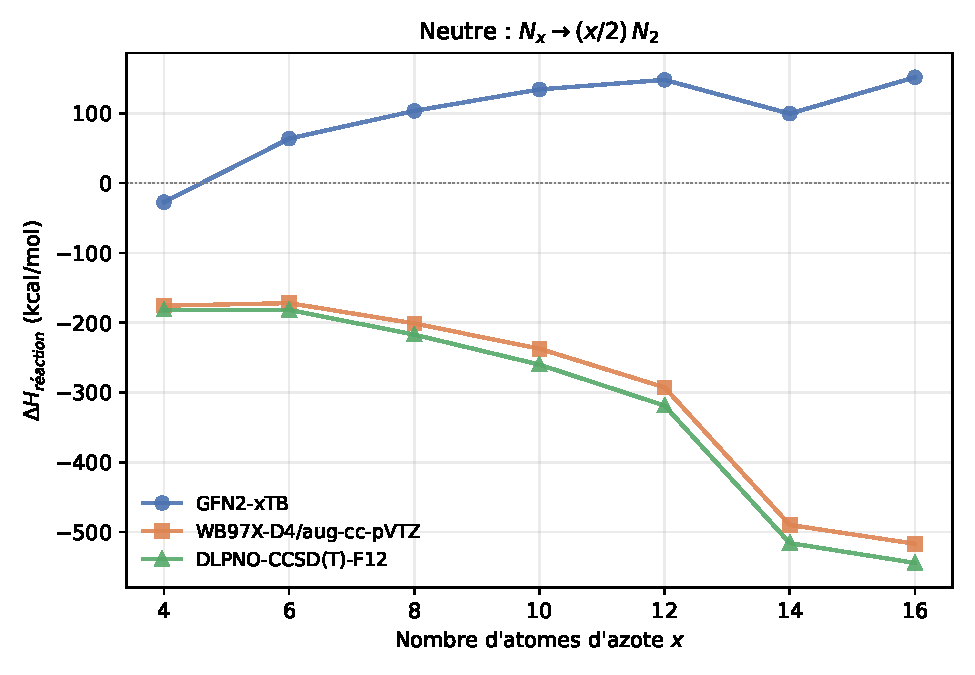
\includegraphics[width=0.75\textwidth]{figures/isodesmic_neutral_N2.pdf}
  \caption{Neutre~: $N_x \to (x/2)\,N_2$.}
\end{figure}

\begin{figure}[H]
  \centering
  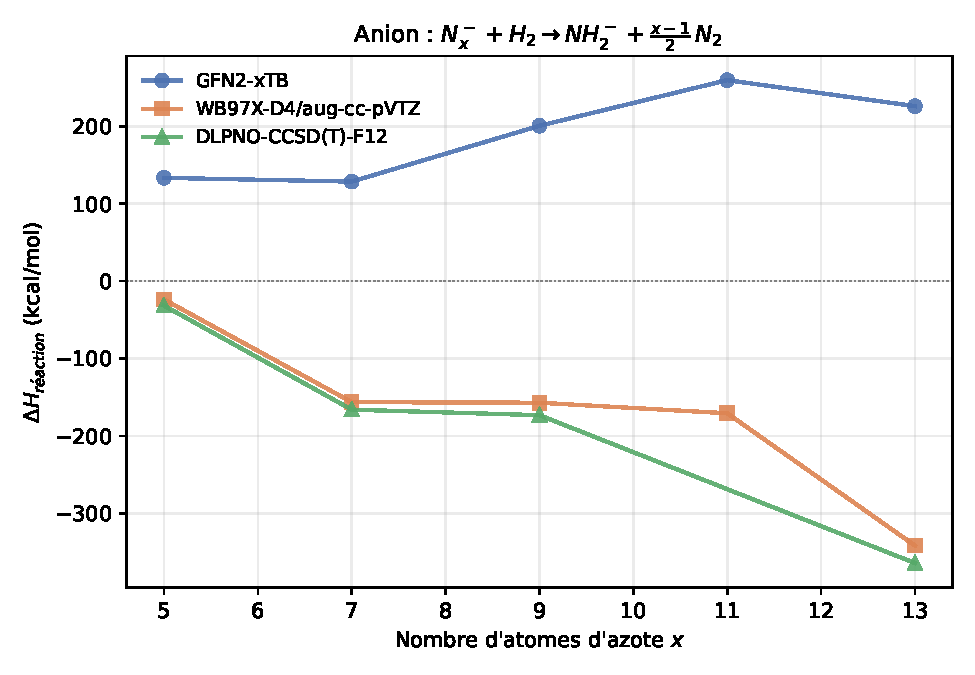
\includegraphics[width=0.75\textwidth]{figures/isodesmic_anion_H2.pdf}
  \caption{Anion, r\'ef\'erence H$_2$/NH$_2^-$.}
\end{figure}

\begin{figure}[H]
  \centering
  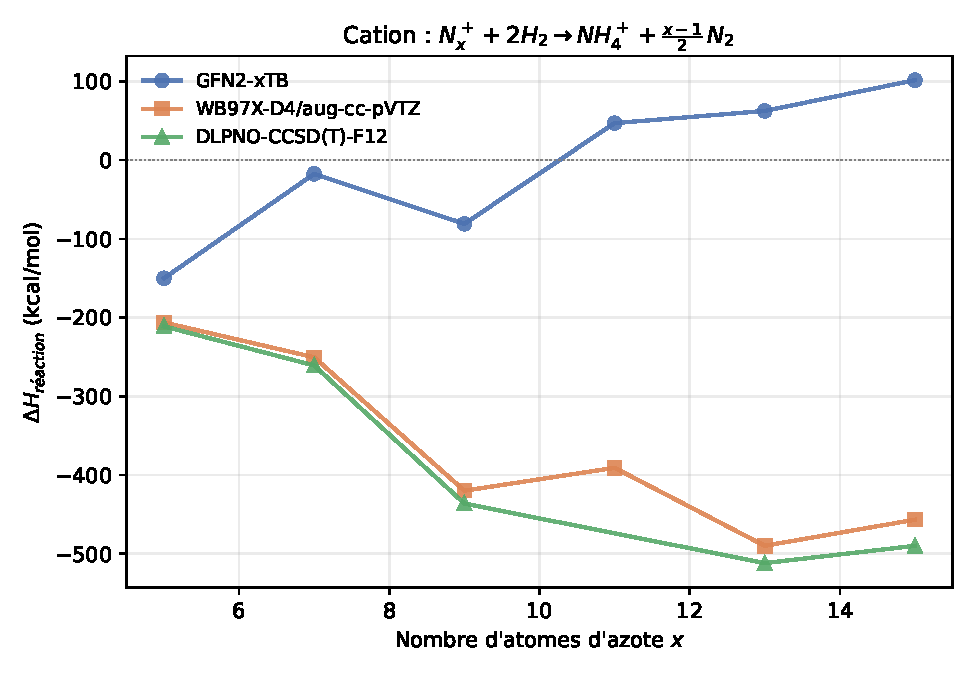
\includegraphics[width=0.75\textwidth]{figures/isodesmic_cation_H2.pdf}
  \caption{Cation, r\'ef\'erence H$_2$/NH$_4^+$.}
\end{figure}

\begin{figure}[H]
  \centering
  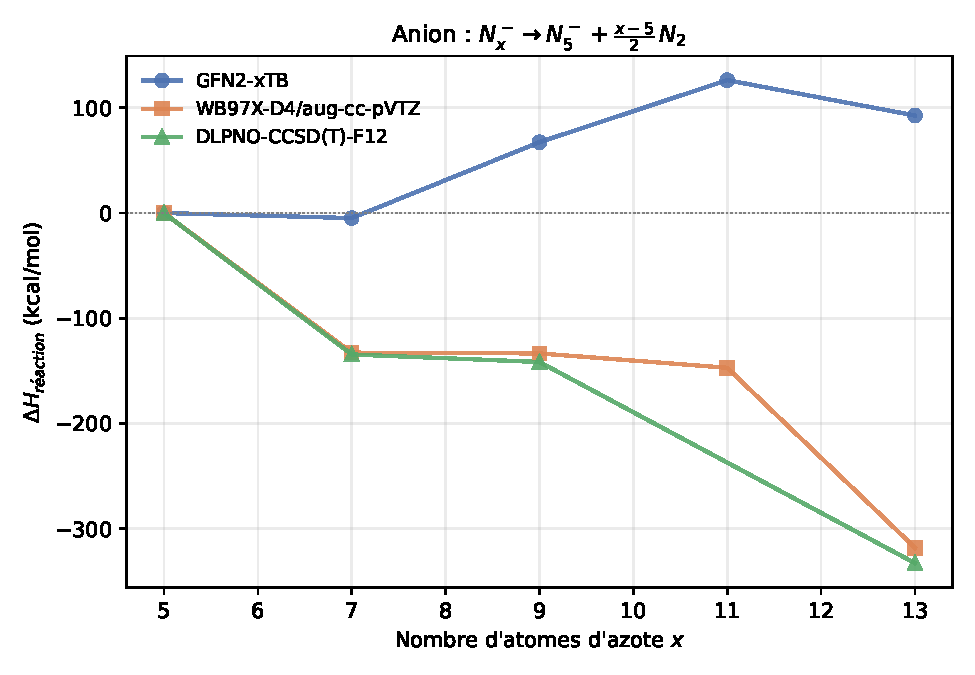
\includegraphics[width=0.75\textwidth]{figures/isodesmic_anion_N5.pdf}
  \caption{Anion, r\'ef\'erence N$_5^-$ ($D_{5h}$).}
\end{figure}

\begin{figure}[H]
  \centering
  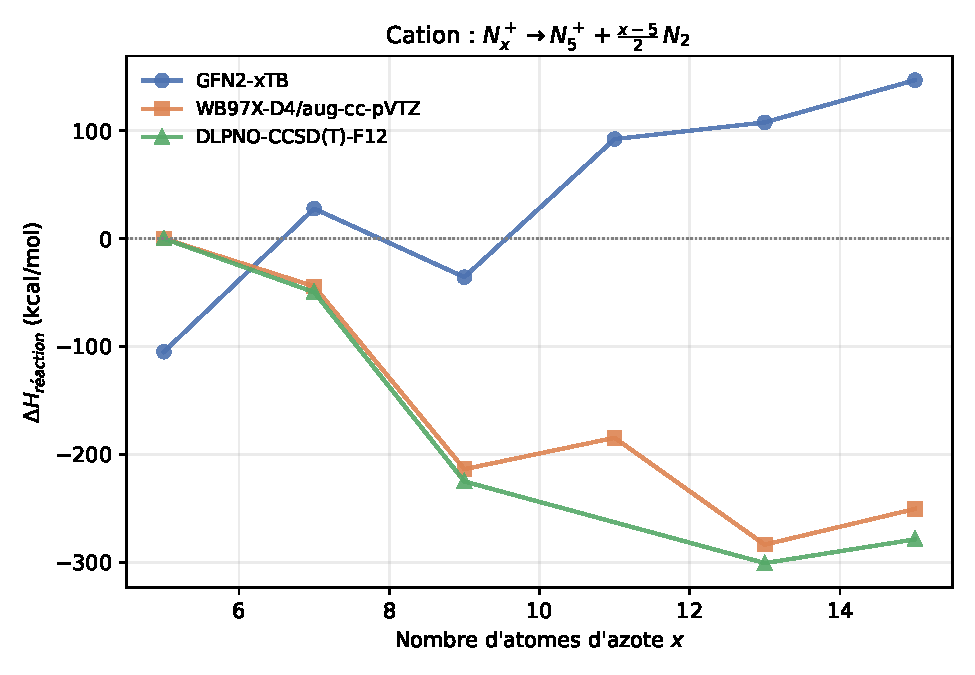
\includegraphics[width=0.75\textwidth]{figures/isodesmic_cation_N5.pdf}
  \caption{Cation, r\'ef\'erence N$_5^+$ ($C_{2v}$).}
\end{figure}

Reproductible via
\texttt{orca\_jobs/report/scripts/build\_isodesmic\_reactions.py}
(lecture seule, aucune d\'ependance \`a un \'etat interm\'ediaire~: \`a
relancer d\`es que la campagne CCSD(T) avance pour \'etendre la
couverture des courbes).

\section{V\'erification des minima}
\label{sec:minima}

Les 193 jobs SLURM de cette campagne sont tous termin\'es, mais
\textbf{35 d'entre eux (18~\%) n'ont pas convergé} -- l'optimiseur DFT a
atteint sa limite de cycles (\texttt{The optimization did not converge
but reached the maximum}) sans trouver de point stationnaire ; leur
\'energie n'est donc pas exploitable en l'\'etat. Un contr\^ole de
connectivit\'e sur la derni\`ere g\'eom\'etrie tent\'ee (et non la
g\'eom\'etrie xTB de d\'epart) montre que \textbf{28 des 35 sont d\'ej\`a
s\'epar\'ees en plusieurs composantes connexes} \`a ce dernier cycle --
l'optimiseur suit une dissociation en cours plut\^ot qu'un vrai probl\`eme
num\'erique de convergence, et une reprise avec plus de cycles ne
trouvera vraisemblablement aucun minimum li\'e pour ces topologies.
Seules les \textbf{7} restantes (cluster unique au dernier cycle) sont
des candidates cr\'edibles \`a une reprise. Liste compl\`ete avec le
nombre de cycles atteint, le statut de fragmentation au dernier cycle et
repr\'esentation avant (g\'eom\'etrie xTB de d\'epart) / dernier cycle
tent\'e~: Tableau~S2 et Figure~S2 (Annexe, \S\ref{sec:si-nonconverged}).
Ces 35 sont exclues de
tous les tableaux d'analyse ci-dessous et devront \^etre reprises avec
davantage de cycles d'optimisation (\texttt{\%geom MaxIter}) dans une
prochaine passe. Les \textbf{158 structures restantes} disposent d'un
bloc de thermochimie complet, parmi lesquelles \textbf{38 pr\'esentent
au moins une fr\'equence imaginaire} et ne sont donc pas, en l'\'etat, de
vrais minima locaux. Contrairement au protocole
gros-cluster, aucune red\'esym\'etrisation automatique n'est appliqu\'ee~:
chaque candidat flagg\'e devra \^etre repris manuellement (distorsion le
long du mode imaginaire puis r\'eoptimisation) avant d'\^etre retenu comme
candidat final -- exactement la logique de la colonne
\texttt{is\_true\_minimum} / \texttt{n\_freq\_hops} d\'ej\`a impl\'ement\'ee
dans \texttt{polyN\_pipeline.py} au niveau GFN2-xTB, appliqu\'ee ici au
niveau DFT. Liste compl\`ete avec la fr\'equence imaginaire dominante
(la plus n\'egative), son intensit\'e IR et l'\'energie relative au
ground-state DFT de la m\^eme composition~: Tableau~S2 (Annexe) -- cette
derni\`ere colonne permet de v\'erifier si l'instabilit\'e vibrationnelle
concentre sur les isom\`eres d\'ej\`a tr\`es haut en \'energie (attendu)
ou touche aussi des candidats proches du ground-state (auquel cas ce
serait plus pr\'eoccupant pour le classement de stabilit\'e).

Un contr\^ole s\'epar\'e de connectivit\'e (composantes connexes du
graphe N--N \`a 1,70~\AA) identifie par ailleurs \textbf{24 candidats
fragment\'es} -- deux ou plusieurs esp\`eces mol\'eculaires distinctes
(ex.\ N$_2$ + N$_3^-$) plut\^ot qu'un cluster N$_x$ li\'e unique, list\'es
\`a part en Tableau~S1 avec repr\'esentation avant/apr\`es en Figure~S1.
Ce contr\^ole a \'et\'e appliqu\'e \'egalement \`a la g\'eom\'etrie de
d\'epart (avant tout calcul DFT) pour les 24~: \textbf{11 \'etaient
d\'ej\`a fragment\'ees dans la g\'eom\'etrie GFN2-xTB issue du criblage},
avant m\^eme d'entrer dans cette campagne DFT (artefact du criblage en
amont, colonne \emph{d\'ej\`a frag.\ \`a xTB} du Tableau~S1) ; les 13
autres \'etaient des clusters intacts \`a xTB et n'ont fragment\'e que
pendant l'optimisation DFT. Les tableaux d'analyse
(\S\ref{sec:provenance}--\ref{sec:bonds}) et la comparaison de stabilit\'e
(\S\ref{sec:litterature}) portent uniquement sur les clusters li\'es~: une
esp\`ece dissoci\'ee est souvent plus basse en \'energie qu'un vrai
cluster li\'e, ce qui fausserait tout classement fond\'e sur l'\'energie
seule.

\section{Orbitales fronti\`eres}

\begin{longtable}{@{}p{4.6cm}p{1.6cm}rrr@{}}
\scriptsize
\caption{Orbitales frontières (WB97X-D4/aug-cc-pVTZ) des candidats termin\'es.}
\label{tab:homolumo}\\
\toprule
\textbf{Nom} & \textbf{PG} & \textbf{HOMO (eV)} & \textbf{LUMO (eV)} & \textbf{Gap (eV)} \\
\midrule\endfirsthead
\multicolumn{5}{c}{\small (suite)}\\ \toprule
\textbf{Nom} & \textbf{PG} & \textbf{HOMO (eV)} & \textbf{LUMO (eV)} & \textbf{Gap (eV)} \\
\midrule\endhead
\bottomrule\endfoot
\bottomrule\endlastfoot
\addlinespace
\texttt{N10\_neutral\_neutral\_001} & C2 & -12.9198 & -0.5398 & 12.3800 \\
\texttt{N10\_neutral\_neutral\_002} & C1 & -11.7475 & -1.3053 & 10.4422 \\
\texttt{N10\_neutral\_neutral\_003} & C1 & -9.9826 & -1.1691 & 8.8135 \\
\texttt{N10\_neutral\_neutral\_004} & C1 & -9.7070 & -1.4443 & 8.2627 \\
\texttt{N10\_neutral\_neutral\_005} & C1 & -10.3189 & -1.6633 & 8.6556 \\
\texttt{N10\_neutral\_neutral\_006} & Cs & -11.2573 & -0.6247 & 10.6326 \\
\texttt{N10\_neutral\_neutral\_007} & Cs & -10.5916 & -1.8512 & 8.7404 \\
\texttt{N10\_neutral\_neutral\_010} & C1 & -11.1858 & -0.6563 & 10.5295 \\
\texttt{N10\_neutral\_neutral\_011} & C1 & -10.2546 & -1.8095 & 8.4451 \\
\texttt{N10\_neutral\_neutral\_013} & C2v & -8.7777 & -2.5200 & 6.2577 \\
\texttt{N10\_neutral\_neutral\_014} & C1 & -10.1760 & -3.1308 & 7.0452 \\
\texttt{N10\_neutral\_neutral\_015} & C2 & -10.7038 & -1.6499 & 9.0539 \\
\texttt{N10\_neutral\_neutral\_016} & C1 & -10.7642 & -1.5672 & 9.1970 \\
\texttt{N10\_neutral\_neutral\_017} & C2v & -11.2487 & -1.3285 & 9.9202 \\
\texttt{N10\_neutral\_neutral\_018} & C2 & -11.1371 & 0.6545 & 11.7916 \\
\texttt{N10\_neutral\_neutral\_019} & C3v & -11.3917 & 0.3446 & 11.7363 \\
\texttt{N10\_neutral\_neutral\_020} & C2 & -10.5955 & -1.4418 & 9.1537 \\
\texttt{N10\_neutral\_neutral\_021} & C2v & -11.2774 & -1.0998 & 10.1776 \\
\texttt{N10\_neutral\_neutral\_022} & D5h & -11.4974 & -0.8667 & 10.6307 \\
\addlinespace
\texttt{N11\_anion\_anion\_001} & C1 & -4.6868 & 4.7575 & 9.4443 \\
\texttt{N11\_anion\_anion\_002} & C1 & -4.6917 & 4.4152 & 9.1069 \\
\texttt{N11\_anion\_anion\_003} & C2 & -4.8000 & 3.0674 & 7.8674 \\
\texttt{N11\_anion\_anion\_004} & C1 & -4.1785 & 4.4585 & 8.6370 \\
\texttt{N11\_anion\_anion\_005} & C1 & -4.0097 & 4.1648 & 8.1745 \\
\texttt{N11\_anion\_anion\_006} & C1 & -4.2089 & 4.0149 & 8.2238 \\
\texttt{N11\_anion\_anion\_007} & Cs & -4.6404 & 4.6470 & 9.2874 \\
\texttt{N11\_anion\_anion\_008} & C1 & -3.9921 & 4.4067 & 8.3988 \\
\texttt{N11\_anion\_anion\_010} & Cs & -3.3157 & 4.1356 & 7.4513 \\
\texttt{N11\_anion\_anion\_011} & C1 & -4.8669 & 2.8826 & 7.7495 \\
\texttt{N11\_anion\_anion\_013} & C1 & -2.7734 & 2.6705 & 5.4439 \\
\texttt{N11\_anion\_anion\_017} & C1 & -4.0058 & 4.4202 & 8.4260 \\
\texttt{N11\_anion\_anion\_018} & C1 & -2.4542 & 3.0647 & 5.5189 \\
\texttt{N11\_cation\_cation\_001} & C2v & -16.4400 & -6.4750 & 9.9650 \\
\texttt{N11\_cation\_cation\_002} & C1 & -15.7017 & -6.1480 & 9.5537 \\
\texttt{N11\_cation\_cation\_004} & C1 & -16.4230 & -7.7299 & 8.6931 \\
\texttt{N11\_cation\_cation\_005} & C2 & -17.0074 & -7.0585 & 9.9489 \\
\texttt{N11\_cation\_cation\_006} & C1 & -15.6724 & -7.1994 & 8.4730 \\
\texttt{N11\_cation\_cation\_007} & C1 & -16.4756 & -7.3306 & 9.1450 \\
\addlinespace
\texttt{N12\_neutral\_neutral\_001} & C1 & -12.3196 & -2.4745 & 9.8451 \\
\texttt{N12\_neutral\_neutral\_002} & C1 & -11.3338 & -2.5898 & 8.7440 \\
\texttt{N12\_neutral\_neutral\_003} & C1 & -11.9678 & -1.5248 & 10.4430 \\
\texttt{N12\_neutral\_neutral\_004} & Cs & -9.8374 & -2.7778 & 7.0596 \\
\texttt{N12\_neutral\_neutral\_005} & C1 & -10.6336 & -1.7561 & 8.8775 \\
\texttt{N12\_neutral\_neutral\_006} & C1 & -10.3193 & -1.8368 & 8.4825 \\
\texttt{N12\_neutral\_neutral\_007} & D3d & -11.6168 & -0.4953 & 11.1215 \\
\texttt{N12\_neutral\_neutral\_008} & C1 & -10.9868 & -0.5129 & 10.4739 \\
\texttt{N12\_neutral\_neutral\_009} & D6h & -10.5865 & -0.9025 & 9.6840 \\
\addlinespace
\texttt{N13\_anion\_anion\_001} & C1 & -4.2327 & 3.0401 & 7.2728 \\
\texttt{N13\_cation\_cation\_001} & C1 & -15.9024 & -7.4824 & 8.4200 \\
\texttt{N13\_cation\_cation\_004} & C1 & -17.1447 & -7.0618 & 10.0829 \\
\addlinespace
\texttt{N14\_neutral\_neutral\_001} & C1 & -9.4477 & -2.1106 & 7.3371 \\
\texttt{N14\_neutral\_neutral\_003} & C2v & -10.3293 & -2.3248 & 8.0045 \\
\texttt{N14\_neutral\_neutral\_004} & C1 & -10.0443 & -1.2482 & 8.7961 \\
\texttt{N14\_neutral\_neutral\_005} & C2 & -12.0686 & 0.6111 & 12.6797 \\
\addlinespace
\texttt{N15\_cation\_cation\_001} & C1 & -16.9221 & -7.4624 & 9.4597 \\
\texttt{N15\_cation\_cation\_002} & C1 & -17.0792 & -5.2422 & 11.8370 \\
\addlinespace
\texttt{N4\_neutral\_neutral\_001} & Td & -13.9405 & 1.7935 & 15.7340 \\
\texttt{N4\_neutral\_neutral\_002} & C2v & -9.2289 & -1.2933 & 7.9356 \\
\texttt{N4\_neutral\_neutral\_003} & C2v & -10.5771 & -1.9734 & 8.6037 \\
\texttt{N4\_neutral\_neutral\_004} & D2h & -10.6441 & -2.3507 & 8.2934 \\
\addlinespace
\texttt{N5\_anion\_anion\_001} & D5h & -5.8838 & 5.8881 & 11.7719 \\
\texttt{N5\_anion\_anion\_002} & C1 & -2.7204 & 5.1388 & 7.8592 \\
\texttt{N5\_anion\_anion\_003} & C1 & -2.7207 & 5.1392 & 7.8599 \\
\texttt{N5\_anion\_anion\_004} & C1 & -2.7202 & 5.1384 & 7.8586 \\
\texttt{N5\_anion\_anion\_005} & C1 & -1.6987 & 5.2393 & 6.9380 \\
\texttt{N5\_anion\_anion\_006} & Cs & -1.8642 & 3.7995 & 5.6637 \\
\texttt{N5\_anion\_anion\_007} & C1 & -1.6984 & 5.2388 & 6.9372 \\
\texttt{N5\_anion\_anion\_008} & C1 & -1.5258 & 4.9909 & 6.5167 \\
\texttt{N5\_anion\_anion\_009} & C1 & -1.5196 & 4.9170 & 6.4366 \\
\texttt{N5\_anion\_anion\_010} & C2v & -1.9078 & 5.4320 & 7.3398 \\
\texttt{N5\_cation\_cation\_001} & C2v & -18.4486 & -6.5903 & 11.8583 \\
\texttt{N5\_cation\_cation\_002} & Cs & -19.4731 & -7.2442 & 12.2289 \\
\texttt{N5\_cation\_cation\_003} & C1 & -18.4487 & -6.5897 & 11.8590 \\
\texttt{N5\_cation\_cation\_004} & C1 & -18.4488 & -6.5881 & 11.8607 \\
\texttt{N5\_cation\_cation\_005} & D2d & -19.7750 & -8.2030 & 11.5720 \\
\texttt{N5\_cation\_cation\_006} & C4v & -20.6577 & -7.9402 & 12.7175 \\
\texttt{N5\_cation\_cation\_007} & C1 & -18.8382 & -10.4353 & 8.4029 \\
\addlinespace
\texttt{N6\_neutral\_neutral\_001} & C2 & -9.2804 & -0.0404 & 9.2400 \\
\texttt{N6\_neutral\_neutral\_002} & D2 & -11.4121 & -2.0522 & 9.3599 \\
\texttt{N6\_neutral\_neutral\_003} & C1 & -10.1854 & -0.1470 & 10.0384 \\
\texttt{N6\_neutral\_neutral\_004} & C1 & -14.8605 & 1.5862 & 16.4467 \\
\texttt{N6\_neutral\_neutral\_005} & C1 & -10.0047 & -1.3166 & 8.6881 \\
\texttt{N6\_neutral\_neutral\_006} & C1 & -9.3271 & -0.6904 & 8.6367 \\
\texttt{N6\_neutral\_neutral\_007} & C2 & -12.1087 & -0.8535 & 11.2552 \\
\texttt{N6\_neutral\_neutral\_008} & C2v & -12.0044 & -0.7828 & 11.2216 \\
\texttt{N6\_neutral\_neutral\_009} & C2 & -11.2453 & -0.2179 & 11.0274 \\
\texttt{N6\_neutral\_neutral\_010} & C2v & -9.7889 & -3.6564 & 6.1325 \\
\texttt{N6\_neutral\_neutral\_012} & D3h & -11.9779 & 0.1531 & 12.1310 \\
\addlinespace
\texttt{N7\_anion\_anion\_001} & C1 & -1.9595 & 4.7108 & 6.6703 \\
\texttt{N7\_anion\_anion\_003} & C2v & -3.1498 & 5.2806 & 8.4304 \\
\texttt{N7\_anion\_anion\_007} & Cs & -2.2941 & 4.1099 & 6.4040 \\
\texttt{N7\_anion\_anion\_008} & C1 & -2.9901 & 4.4265 & 7.4166 \\
\texttt{N7\_anion\_anion\_009} & C1 & -3.0117 & 4.5488 & 7.5605 \\
\texttt{N7\_anion\_anion\_010} & C2v & -4.2100 & 5.1843 & 9.3943 \\
\texttt{N7\_anion\_anion\_011} & C1 & -2.2849 & 4.8177 & 7.1026 \\
\texttt{N7\_anion\_anion\_012} & C1 & -2.2126 & 4.8717 & 7.0843 \\
\texttt{N7\_anion\_anion\_013} & C1 & -3.7378 & 4.5618 & 8.2996 \\
\texttt{N7\_anion\_anion\_014} & Cs & -3.7877 & 5.0235 & 8.8112 \\
\texttt{N7\_anion\_anion\_016} & C1 & -3.5935 & 4.2032 & 7.7967 \\
\texttt{N7\_anion\_anion\_017} & Cs & -4.3231 & 4.7093 & 9.0324 \\
\texttt{N7\_anion\_anion\_018} & Cs & -2.9551 & 4.2456 & 7.2007 \\
\texttt{N7\_anion\_anion\_019} & C1 & -2.6908 & 5.1080 & 7.7988 \\
\texttt{N7\_anion\_anion\_020} & C1 & -3.1082 & 2.6928 & 5.8010 \\
\texttt{N7\_cation\_cation\_001} & Cs & -16.8094 & -7.0687 & 9.7407 \\
\texttt{N7\_cation\_cation\_003} & Cs & -18.3210 & -7.6492 & 10.6718 \\
\texttt{N7\_cation\_cation\_005} & Cs & -17.9319 & -10.5556 & 7.3763 \\
\texttt{N7\_cation\_cation\_006} & C1 & -19.0163 & -9.2300 & 9.7863 \\
\addlinespace
\texttt{N8\_neutral\_neutral\_001} & D2h & -11.2755 & -0.0572 & 11.2183 \\
\texttt{N8\_neutral\_neutral\_002} & C1 & -11.0090 & -0.5306 & 10.4784 \\
\texttt{N8\_neutral\_neutral\_003} & C1 & -9.8865 & 0.0206 & 9.9071 \\
\texttt{N8\_neutral\_neutral\_005} & C2 & -9.6080 & -0.0360 & 9.5720 \\
\texttt{N8\_neutral\_neutral\_009} & D3h & -11.7827 & -1.2276 & 10.5551 \\
\texttt{N8\_neutral\_neutral\_010} & Cs & -9.8734 & -1.8161 & 8.0573 \\
\texttt{N8\_neutral\_neutral\_016} & Cs & -11.5952 & -0.6090 & 10.9862 \\
\texttt{N8\_neutral\_neutral\_019} & D2d & -12.0840 & -1.8861 & 10.1979 \\
\texttt{N8\_neutral\_neutral\_024} & D2h & -9.2373 & -1.2856 & 7.9517 \\
\addlinespace
\texttt{N9\_anion\_anion\_001} & C1 & -3.3287 & 4.4403 & 7.7690 \\
\texttt{N9\_anion\_anion\_006} & Cs & -4.5780 & 4.6285 & 9.2065 \\
\texttt{N9\_cation\_cation\_001} & C1 & -18.1169 & -6.2607 & 11.8562 \\
\end{longtable}

\section{Charges atomiques}

Charges de Mulliken et L\"owdin, natives \`a ORCA. Les charges de Bader
(QTAIM) et de Manz (DDEC6) restent report\'ees (\S\ref{sec:limites}) --
ni l'une ni l'autre n'est native \`a ORCA.

\begin{longtable}{@{}p{4.6cm}rrrp{2.6cm}@{}}
\scriptsize
\caption{Charges atomiques (Mulliken et L\"owdin) du meilleur minimum confirm\'e de chaque groupe (formule, charge) -- min/max sur les atomes N. Charges de Bader/QTAIM non natives \`a ORCA, report\'ees (\S\ref{sec:limites}).}
\label{tab:charges}\\
\toprule
\textbf{Nom} & \textbf{Mulliken min} & \textbf{Mulliken max} & \textbf{L\"owdin min/max} & \\
\midrule\endfirsthead
\multicolumn{4}{c}{\small (suite)}\\ \toprule\endhead
\bottomrule\endfoot
\bottomrule\endlastfoot
\texttt{N4\_neutral\_neutral\_001} & -0.000 & 0.000 & -0.000 / 0.000 & \\
\texttt{N5\_anion\_anion\_002} & -0.879 & 0.791 & -0.792 / -0.019 & \\
\texttt{N5\_cation\_cation\_001} & -0.409 & 0.929 & -0.069 / 0.465 & \\
\texttt{N6\_neutral\_neutral\_001} & -0.552 & 1.088 & -0.280 / 0.279 & \\
\texttt{N7\_anion\_anion\_011} & -0.844 & 1.113 & -0.385 / 0.112 & \\
\texttt{N7\_cation\_cation\_001} & -0.296 & 1.030 & -0.060 / 0.447 & \\
\texttt{N9\_anion\_anion\_001} & -0.818 & 1.443 & -0.568 / 0.159 & \\
\texttt{N9\_cation\_cation\_001} & -0.501 & 1.052 & -0.105 / 0.448 & \\
\texttt{N10\_neutral\_neutral\_001} & -0.282 & 0.818 & -0.303 / 0.133 & \\
\texttt{N11\_anion\_anion\_006} & -0.756 & 1.131 & -0.375 / 0.197 & \\
\texttt{N11\_cation\_cation\_001} & -0.656 & 1.068 & -0.235 / 0.410 & \\
\texttt{N12\_cation\_cation\_001} & -0.169 & 1.074 & -0.269 / 0.207 & \\
\texttt{N12\_neutral\_neutral\_001} & -0.319 & 1.408 & -0.380 / 0.154 & \\
\texttt{N13\_anion\_anion\_001} & -0.979 & 1.392 & -0.394 / 0.224 & \\
\texttt{N13\_cation\_cation\_001} & -0.293 & 0.835 & -0.181 / 0.218 & \\
\texttt{N14\_neutral\_neutral\_005} & -0.211 & 0.218 & -0.121 / 0.073 & \\
\texttt{N15\_cation\_cation\_001} & -0.422 & 0.873 & -0.258 / 0.419 & \\
\end{longtable}

\section{Distances et ordres de liaison N--N~: corr\'elation avec $\Delta H_f$}
\label{sec:bonds}

Pour les compos\'es neutres, proportion de liaisons courtes (triple,
double, ou d\'elocalis\'ees ${\sim}1{,}5$) parmi les liaisons r\'eelles, et
ordre de Mayer moyen, en regard du $\Delta H_f$ GFN2-xTB. Tendance
attendue~: davantage de caract\`ere multiple devrait corr\'eler avec un
$\Delta H_f$ plus \'elev\'e (structures plus contraintes, moins proches de
2~N$_2$) -- \`a confirmer statistiquement une fois la campagne DFT
compl\`ete (l'\'echantillon actuel, 45 structures neutres, montre la
tendance qualitativement mais reste bruit\'e).

{\scriptsize
\begin{longtable}{@{}p{4.6cm}rrrp{2.4cm}r@{}}
\caption{Compos\'es \textbf{neutres} termin\'es : proportion de liaisons N--N courtes (triple/double/d\'elocalis\'ees) parmi les liaisons r\'eelles (hors contacts non-liants), et $\Delta H_f$ GFN2-xTB. Seuils de classification en \S\ref{sec:limites} de \texttt{harvest\_results.py}.}
\label{tab:bonds-dhf}\\
\toprule
\textbf{Nom} & \textbf{liaisons} & \textbf{BO Mayer moy.} & \textbf{\% courtes\footnotemark[1]} & \textbf{classes pr\'esentes} & \textbf{$\Delta H_f^{xtb}$} \\
\midrule\endfirsthead
\multicolumn{6}{c}{\small (suite)}\\ \toprule
\textbf{Nom} & \textbf{liaisons} & \textbf{BO Mayer moy.} & \textbf{\% courtes} & \textbf{classes pr\'esentes} & \textbf{$\Delta H_f^{xtb}$} \\
\midrule\endhead
\bottomrule\endfoot
\bottomrule\endlastfoot
\texttt{N10\_neutral\_neutral\_001} & 11 & 0.806 & 36\% & delocalized 1.5, single & -134.2 \\
\texttt{N10\_neutral\_neutral\_002} & 10 & 0.917 & 70\% & delocalized 1.5, single, triple & -123.7 \\
\texttt{N10\_neutral\_neutral\_003} & 9 & 1.071 & 67\% & delocalized 1.5, single, triple & -110.7 \\
\texttt{N10\_neutral\_neutral\_004} & 10 & 0.829 & 60\% & delocalized 1.5, single, triple & -100.84 \\
\texttt{N10\_neutral\_neutral\_005} & 10 & 0.937 & 50\% & delocalized 1.5, double, single & -97.64 \\
\texttt{N10\_neutral\_neutral\_006} & 12 & 0.792 & 25\% & double, single & -95.64 \\
\texttt{N10\_neutral\_neutral\_007} & 11 & 0.790 & 36\% & delocalized 1.5, single & -80.55 \\
\texttt{N10\_neutral\_neutral\_010} & 12 & 0.772 & 25\% & delocalized 1.5, single & -45.58 \\
\texttt{N10\_neutral\_neutral\_011} & 11 & 0.787 & 45\% & delocalized 1.5, double, single & -41.25 \\
\texttt{N10\_neutral\_neutral\_013} & 12 & 0.643 & 33\% & delocalized 1.5, single & -34.65 \\
\texttt{N10\_neutral\_neutral\_014} & 12 & 0.713 & 42\% & delocalized 1.5, long/weak, single & -33.7 \\
\texttt{N10\_neutral\_neutral\_015} & 12 & 0.768 & 25\% & delocalized 1.5, single & -22.96 \\
\texttt{N10\_neutral\_neutral\_016} & 12 & 0.760 & 25\% & delocalized 1.5, double, single & -20.37 \\
\texttt{N10\_neutral\_neutral\_017} & 13 & 0.733 & 15\% & double, single & -3.74 \\
\texttt{N10\_neutral\_neutral\_018} & 15 & 0.658 & 0\% & single & 8.82 \\
\texttt{N10\_neutral\_neutral\_019} & 15 & 0.666 & 0\% & single & 13.77 \\
\texttt{N10\_neutral\_neutral\_020} & 14 & 0.671 & 7\% & delocalized 1.5, single & 34.26 \\
\texttt{N10\_neutral\_neutral\_021} & 13 & 0.781 & 15\% & delocalized 1.5, single & 40.4 \\
\texttt{N10\_neutral\_neutral\_022} & 15 & 0.663 & 0\% & single & 49.74 \\
\texttt{N12\_neutral\_neutral\_001} & 13 & 0.615 & 38\% & delocalized 1.5, single & -147.92 \\
\texttt{N12\_neutral\_neutral\_002} & 13 & 0.700 & 62\% & delocalized 1.5, single & -134.68 \\
\texttt{N12\_neutral\_neutral\_003} & 13 & 0.801 & 69\% & delocalized 1.5, double, single & -112.01 \\
\texttt{N12\_neutral\_neutral\_004} & 13 & 0.695 & 38\% & delocalized 1.5, single & -102.34 \\
\texttt{N12\_neutral\_neutral\_005} & 14 & 0.760 & 29\% & double, single & -79.39 \\
\texttt{N12\_neutral\_neutral\_006} & 14 & 0.722 & 29\% & delocalized 1.5, double, single & -71.56 \\
\texttt{N12\_neutral\_neutral\_007} & 18 & 0.645 & 0\% & single & -46.96 \\
\texttt{N12\_neutral\_neutral\_008} & 15 & 0.787 & 20\% & delocalized 1.5, single & -14.76 \\
\texttt{N12\_neutral\_neutral\_009} & 18 & 0.605 & 0\% & single & 94.51 \\
\texttt{N14\_neutral\_neutral\_001} & 16 & 0.599 & 50\% & delocalized 1.5, single & -140.21 \\
\texttt{N14\_neutral\_neutral\_003} & 17 & 0.702 & 24\% & delocalized 1.5, double, single & -62.32 \\
\texttt{N14\_neutral\_neutral\_005} & 21 & 0.681 & 0\% & long/weak, single & -6.87 \\
\texttt{N4\_neutral\_neutral\_001} & 6 & 0.796 & 0\% & single & 27.32 \\
\texttt{N4\_neutral\_neutral\_002} & 4 & 1.118 & 50\% & delocalized 1.5, double, single & 53.79 \\
\texttt{N4\_neutral\_neutral\_003} & 5 & 0.841 & 0\% & long/weak, single & 58.33 \\
\texttt{N4\_neutral\_neutral\_004} & 4 & 1.056 & 50\% & delocalized 1.5, single & 68.96 \\
\texttt{N6\_neutral\_neutral\_001} & 5 & 1.248 & 80\% & delocalized 1.5, single, triple & -63.71 \\
\texttt{N6\_neutral\_neutral\_002} & 6 & 0.835 & 100\% & delocalized 1.5 & -39.62 \\
\texttt{N6\_neutral\_neutral\_003} & 6 & 1.112 & 50\% & delocalized 1.5, double, single, triple & -8.71 \\
\texttt{N6\_neutral\_neutral\_005} & 6 & 1.071 & 67\% & delocalized 1.5, long/weak, triple & 0.91 \\
\texttt{N6\_neutral\_neutral\_006} & 6 & 1.133 & 67\% & delocalized 1.5, long/weak, single, triple & 15.09 \\
\texttt{N6\_neutral\_neutral\_007} & 7 & 0.867 & 29\% & delocalized 1.5, single & 19.92 \\
\texttt{N6\_neutral\_neutral\_008} & 8 & 0.790 & 12\% & double, single & 20.81 \\
\texttt{N6\_neutral\_neutral\_009} & 7 & 0.979 & 29\% & double, single & 47.09 \\
\texttt{N6\_neutral\_neutral\_010} & 6 & 0.935 & 33\% & single, triple & 50.62 \\
\texttt{N6\_neutral\_neutral\_012} & 9 & 0.729 & 0\% & single & 72.95 \\
\texttt{N8\_neutral\_neutral\_001} & 9 & 0.698 & 56\% & delocalized 1.5, single & -113.38 \\
\texttt{N8\_neutral\_neutral\_002} & 8 & 0.891 & 75\% & delocalized 1.5, single, triple & -103.47 \\
\texttt{N8\_neutral\_neutral\_003} & 7 & 1.024 & 71\% & delocalized 1.5, single, triple & -93.12 \\
\texttt{N8\_neutral\_neutral\_005} & 7 & 1.158 & 71\% & delocalized 1.5, single, triple & -83.97 \\
\texttt{N8\_neutral\_neutral\_009} & 9 & 0.806 & 33\% & double, single & -39.68 \\
\texttt{N8\_neutral\_neutral\_010} & 8 & 0.910 & 50\% & delocalized 1.5, single, triple & -29.32 \\
\texttt{N8\_neutral\_neutral\_016} & 11 & 0.743 & 9\% & delocalized 1.5, single & 19.4 \\
\texttt{N8\_neutral\_neutral\_019} & 10 & 0.828 & 20\% & double, single & 36.92 \\
\texttt{N8\_neutral\_neutral\_024} & 11 & 0.618 & 18\% & delocalized 1.5, long/weak, single & 69.67 \\
\end{longtable}
\footnotetext[1]{Triple, double ou d\'elocalis\'ee (ordre ${\sim}1{,}5$), \`a l'exclusion des liaisons simples et des contacts non-liants.}
\noindent{\footnotesize\textit{Note~:} $\Delta H_f^{xtb}$ (compos\'es \textbf{neutres} uniquement, cette table) est calcul\'e pour la r\'eaction $(n/2)\,\mathrm{N}_2 \rightarrow \mathrm{N}_n$, soit $\Delta H_f = E(\mathrm{N}_n) - (n/2)\,E(\mathrm{N}_2)$, r\'ef\'erence $\Delta H_f(\mathrm{N}_2)=0$. C'est une d\'efinition \textbf{diff\'erente} de celle utilis\'ee pour les cations/anions (Tableaux~3--4, \S\ref{sec:provenance})~: $\mathrm{N}_5^{-}$(D$_{5h}$)$~+~((n-5)/2)\,\mathrm{N}_2 \rightarrow \mathrm{N}_n^{-}$ et $\mathrm{N}_5^{+}$(C$_{2v}$)$~+~((n-5)/2)\,\mathrm{N}_2 \rightarrow \mathrm{N}_n^{+}$, ancr\'ees sur les $\Delta H_f$ litt\'erature de $\mathrm{N}_5^{-}$/$\mathrm{N}_5^{+}$ (valeurs \S\ref{sec:provenance}) plut\^ot que sur N$_2$ seul -- les deux d\'efinitions ne sont pas directement comparables entre elles.}
}

\section{Confrontation \`a la litt\'erature et aux bases externes}
\label{sec:litterature}

Deux ensembles distincts sont compar\'es ici. \textbf{Nos 193 candidats}
sont le jeu DFT WB97X-D4 de ce rapport~: structures issues du criblage
GFN2-xTB de \texttt{polyN-pipeline} (§\ref{sec:origine}, Tableaux~2--4).
\textbf{337 structures connues} d\'esigne un ensemble s\'epar\'e~: le
fichier \texttt{biblio\_polyN/comparison\_table\_3sources.csv} de
\texttt{polyN-pipeline}, qui catalogue des structures tir\'ees d'articles
publi\'es et des bases externes \texttt{N\_csp} et \texttt{polyN\_study},
toutes relax\'ees ind\'ependamment au m\^eme niveau GFN2-xTB pour permettre
la comparaison. Le croisement par (N, charge) entre nos 193 candidats et
ces 337 r\'ef\'erences donne trois r\'esultats compl\'ementaires~:

\begin{itemize}[leftmargin=1.4em]
  \item \textbf{Couverture} : 12 des 19 groupes (89 des 193 structures,
  46~\%) n'ont \textbf{aucune} r\'ef\'erence catalogu\'ee \`a cette
  formule/charge.
  \item \textbf{Topologie} : pour les 104 candidats des 7 groupes
  comparables, une empreinte de graphe de liaisons (s\'equence de degr\'es
  + tailles de cycles + nombre de liaisons, seuil 1,90~\AA, NetworkX)
  montre que 76 (73~\%) ne correspondent \`a aucune connectivit\'e
  catalogu\'ee. Au total, \textbf{165 des 193 candidats (86~\%)} sont donc
  distincts de tout ce qui existe dans le tableau \`a 3 sources.
  \item \textbf{Stabilit\'e} : 3 des 7 groupes comparables voient leur
  meilleur candidat local d\'epasser en stabilit\'e le meilleur catalogu\'e
  -- N$_9^-$ ($-0{,}166$~eV/atome), N$_{10}$ ($-0{,}066$, malgr\'e 60
  r\'ef\'erences disponibles), N$_{12}$ ($-0{,}246$). N$_6$ et N$_8$
  retombent exactement sur le minimum d\'ej\`a connu. N$_4$ est la seule
  perte nette ($+0{,}302$~eV/atome).
  N$_9^+$ : le seul candidat termin\'e \`a cette composition
  (\texttt{N9\_cation\_cation\_001}) est fragment\'e en trois esp\`eces
  s\'epar\'ees (2+2+5 atomes, Tableau~S1) -- aucune comparaison de
  stabilit\'e n'est possible pour ce groupe tant qu'un candidat
  non-fragment\'e n'a pas termin\'e.
\end{itemize}

D\'etail complet et graphique interactif : voir l'artefact
\href{https://claude.ai/code/artifact/da2b875a-5560-4a2d-b719-5dbb4d27ddac}{\emph{Uncharted Compositions}}.

\section{Couverture du criblage et pistes de compl\'ement}
\label{sec:coverage}

Les 193 candidats proviennent exclusivement du pool~1 (criblage
combinatoire/substitution, \S\ref{sec:pools}) ; le pool~2 (surrogate
adaptatif \texttt{polyN\_adapt}) n'a contribu\'e aucun candidat \`a ce
jeu. Le tableau suivant d\'ecompose, pour chaque groupe (N, charge)
effectivement \'echantillonn\'e, le nombre de structures g\'en\'er\'ees et
leur devenir apr\`es DFT.

{\scriptsize
\begin{longtable}{@{}ccrrrrrr@{}}
\caption{Couverture du criblage pool~1 (\texttt{polyN-pipeline}, g\'en\'eration combinatoire/substitution, \S\ref{sec:pools}) par groupe (N, charge). \emph{Rendement} = confirm\'e / g\'en\'er\'e. Groupes \`a 0 candidat surlign\'es par un tiret.}
\label{tab:coverage}\\
\toprule
\textbf{N} & \textbf{Charge} & \textbf{G\'en\'er\'e} & \textbf{Confirm\'e} & \textbf{Rendement} & \textbf{Frag.} & \textbf{Imag.} & \textbf{Non conv.} \\
\midrule\endfirsthead
\multicolumn{8}{c}{\small (suite)}\\ \toprule\endhead
\bottomrule\endfoot
\bottomrule\endlastfoot
\addlinespace
4 & 0 & 4 & 2 & 50\% & 0 & 2 & 0 \\
\addlinespace
5 & + & 7 & 6 & 86\% & 1 & 0 & 0 \\
5 & - & 10 & 2 & 20\% & 7 & 1 & 0 \\
\addlinespace
6 & 0 & 12 & 9 & 75\% & 1 & 1 & 1 \\
\addlinespace
7 & + & 6 & 2 & 33\% & 0 & 2 & 2 \\
7 & - & 20 & 10 & 50\% & 0 & 8 & 2 \\
\addlinespace
8 & 0 & 25 & 19 & 76\% & 2 & 1 & 3 \\
\addlinespace
9 & + & 12 & 4 & 33\% & 1 & 1 & 6 \\
9 & - & 20 & 11 & 55\% & 1 & 2 & 6 \\
\addlinespace
10 & 0 & 22 & 18 & 82\% & 0 & 1 & 3 \\
\addlinespace
11 & + & 10 & 4 & 40\% & 2 & 2 & 2 \\
11 & - & 18 & 5 & 28\% & 2 & 6 & 5 \\
\addlinespace
12 & 0 & 9 & 8 & 89\% & 0 & 1 & 0 \\
12 & + & 1 & 1 & 100\% & 0 & 0 & 0 \\
\addlinespace
13 & + & 4 & 2 & 50\% & 0 & 0 & 2 \\
13 & - & 4 & 1 & 25\% & 0 & 0 & 3 \\
\addlinespace
14 & 0 & 5 & 3 & 60\% & 1 & 1 & 0 \\
\addlinespace
15 & + & 2 & 2 & 100\% & 0 & 0 & 0 \\
\addlinespace
16 & 0 & 2 & 1 & 50\% & 0 & 1 & 0 \\
\end{longtable}
}

\textbf{Hors p\'erim\`etre singulet} (0 candidat, et cela ne changera pas avec un g\'en\'erateur singulet -- pool~1 ou pool~2 : $7N-\mathrm{charge}$ impair, aucun \'etat singulet n'existe \`a cette taille/charge, il faudrait un doublet)~: N$_{4}^{-}$, N$_{4}^{+}$, N$_{5}$, N$_{6}^{-}$, N$_{6}^{+}$, N$_{7}$, N$_{8}^{-}$, N$_{8}^{+}$, N$_{9}$, N$_{10}^{-}$, N$_{10}^{+}$, N$_{11}$, N$_{12}^{-}$, N$_{13}$, N$_{14}^{-}$, N$_{14}^{+}$, N$_{15}$, N$_{16}^{-}$, N$_{16}^{+}$.\\[4pt]\textbf{Trou de couverture r\'eellement accessible} (0 candidat mais compatible singulet -- cible l\'egitime pour un compl\'ement pool~1 ou pool~2)~: N$_{15}^{-}$.\\[4pt]\textbf{Rendement faible} ($<$40\%, beaucoup de candidats g\'en\'er\'es mais peu confirm\'es -- g\'eom\'etries de d\'epart chimiquement peu viables plut\^ot qu'un manque de volume)~: N$_{5}^{-}$ (2/10, 20\%), N$_{13}^{-}$ (1/4, 25\%), N$_{11}^{-}$ (5/18, 28\%), N$_{7}^{+}$ (2/6, 33\%), N$_{9}^{+}$ (4/12, 33\%).

La quasi-totalit\'e des groupes \`a z\'ero candidat (19 sur 20) sont en
fait \textbf{hors de port\'ee de tout g\'en\'erateur singulet}, pool~1
comme pool~2~: \texttt{core.geng\_interface.validate\_n\_for\_charge}
(pool~2) formalise la r\`egle d\'ej\`a \`a l'oeuvre dans ce criblage
(\S\ref{sec:origine})~: un \'etat singulet n'existe que si $7N-\mathrm{charge}$
est pair, soit $N$ pair pour les neutres et $N$ impair pour les
cations/anions. Les charges paires (N$_x^{+}$/N$_x^{-}$, $x$ pair) et les
neutres \`a $N$ impair sont donc chimiquement exclus en singulet quelle
que soit la m\'ethode de g\'en\'eration -- il faudrait un doublet, hors
p\'erim\`etre des deux pools actuels (\texttt{evaluation/xtb\_bridge.py}
fixe explicitement la multiplicit\'e \`a 1). \textbf{Un seul groupe est
un vrai trou de couverture accessible en singulet~: N$_{15}^-$}, jamais
\'echantillonn\'e par le pool~1. C'est l\`a, et sur les autres tailles
$\ge$14 compatibles (charges impaires, \texttt{geng}/nauty devenant
co\^uteux \`a partir de $n{\sim}14$--16 selon le README de
\texttt{polyN\_adapt}), que le pool~2 (mutation locale de l'archive
plut\^ot qu'\'enum\'eration compl\`ete) apporte une valeur r\'eelle --
pas en ouvrant de nouvelles charges, mais en couvrant plus efficacement
la m\^eme grille aux grandes tailles. \`A l'inverse, les groupes \`a
rendement faible (N$_5^-$, N$_7^+$, N$_9^+$, N$_{11}^-$, N$_{13}^-$)
restent dans la zone confortable du pool~1 (N$\le$13) mais souffrent
d'un fort taux d'attrition apr\`es DFT (fragmentation, fr\'equence
imaginaire, non-convergence) -- signe que les g\'eom\'etries de d\'epart
g\'en\'er\'ees pour ces formules sont chimiquement peu viables plut\^ot
qu'un simple manque de volume~: un r\'e-\'echantillonnage pool~1 cibl\'e
sur ces groupes pr\'ecis (plut\^ot qu'un changement de g\'en\'erateur)
est la piste la plus directe. Mise \`a jour post\'erieure \`a la r\'edaction
initiale de cette section~: le pool~2 (\texttt{GenerPolyN}) dispose
d\'esormais d'une \'evaluation parall\'elis\'ee par candidat
(\texttt{ProcessPoolExecutor}, jusqu'\`a 40 c\oe urs utilis\'es en
pratique) -- l'affirmation initiale d'une \'evaluation strictement
s\'equentielle mono-c\oe ur ne tient plus.

\textbf{Premi\`ere contribution confirm\'ee du pool~2 au jeu de
structures DFT} (nuit du 6 au 7 septembre 2026) : une campagne DFTB+
ind\'ependante (SCC-DFTB, \texttt{polynitrogen\_charged\_explore.py},
rapatri\'ee d'une exploration ant\'erieure sur Mac) a identifi\'e 13
topologies N$_5$/N$_7$/N$_9$ (charges $\pm1$) absentes du pool DFT
existant (comparaison par isomorphisme de graphe, pas seulement
l'\'etiquette de topologie). Un contr\^ole crois\'e syst\'ematique par
GFN2-xTB (m\^eme protocole que le reste de ce projet, jamais les
\'energies DFTB+ elles-m\^emes) n'en a laiss\'e survivre que 2 sur 13~:
11 pr\'esentaient une fr\'equence imaginaire ou un r\'earrangement d\`es
ce niveau -- confirmation que DFTB+ et GFN2-xTB divergent fortement sur
la stabilit\'e de ces topologies. Des 2 survivantes, soumises en DFT
WB97X-D4 (Opt+Freq, 16~c\oe urs, N$_9^+$)~: l'une n'a pas converg\'e
(limite de cycles atteinte, m\^eme statut que les candidats non
convergés d\'ej\`a exclus de ce rapport), l'autre a converg\'e proprement
mais vers une g\'eom\'etrie \textbf{fragment\'ee} (2+7 atomes) -- aucune
des deux n'int\`egre donc le pool confirm\'e. En parall\`ele, le pipeline
s\'equentiel propre \`a \texttt{GenerPolyN} (croissance par paires
N$_2$ depuis l'archive xTB, \S\ref{sec:pools}) a produit ind\'ependamment
une nouvelle topologie N$_9^-$ (\texttt{N9\_anion\_anion\_021}), confirm\'ee
par le m\^eme protocole DFT complet~: convergence propre, z\'ero
fr\'equence imaginaire, structure intacte. Le pool de structures DFT
confirm\'ees passe ainsi de 110 \`a \textbf{111}. Bilan honn\^ete~: sur
cette premi\`ere nuit, la voie DFTB+$\to$xTB$\to$DFT n'a produit aucune
structure confirm\'ee (0/13), tandis que la croissance interne du
pool~2 en a produit une -- l'exploration ind\'ependante par une
seconde m\'ethode de g\'en\'eration a surtout servi, ici, \`a
\'eliminer des candidats plut\^ot qu'\`a en confirmer.

\textbf{Correctif et campagne \'elargie du pool~2} (nuit du 6 au 7
septembre 2026) : un diagnostic sur la campagne N$_{15}^-$ (\texttt{geng},
seul trou de couverture \`a z\'ero candidat identifi\'e ci-dessus) a
r\'ev\'el\'e une sursouscription OpenMP -- \texttt{evaluation/xtb\_bridge.py}
initialise le runtime OpenMP de \texttt{tblite} dans le processus parent
avant que \texttt{ProcessPoolExecutor} ne cr\'ee ses workers (mode
\texttt{fork}), chaque worker h\'eritant alors d'un runtime d\'ej\`a
configur\'e sur "tous les c\oe urs disponibles" -- mesur\'e : $\sim$30
candidats \'evalu\'es en 13h30 au lieu de quelques minutes attendues.
Corrig\'e par un contexte \texttt{spawn} pour \texttt{ProcessPoolExecutor}
(chaque worker est un interpr\`ete neuf, les variables d'environnement de
threading sont prises en compte d\`es le premier import de \texttt{tblite}),
avec ajout d'un m\'ecanisme de point de sauvegarde/reprise par
g\'en\'eration compl\`ete et d'un suivi d'\'etapes en temps r\'eel. Six
campagnes ont ensuite \'et\'e lanc\'ees en parall\`ele sur autant de
n\oe uds SLURM libres, ciblant N$_{15}^-$ (trou de couverture) et les
groupes \`a rendement faible identifi\'es plus haut (N$_5^-$, N$_7^+$,
N$_9^+$, N$_{11}^-$, N$_{13}^-$). Deux campagnes achev\'ees \`a ce stade,
toutes deux valid\'ees par isomorphisme de graphe contre le pool DFT
confirm\'e : N$_5^-$ retrouve exactement le cycle \texttt{ring-5} d\'ej\`a
connu ; N$_7^+$ retrouve exactement les deux topologies d\'ej\`a
confirm\'ees (\texttt{chain} et \texttt{ring-5-subst}) -- aucune nouvelle
structure sur ces deux compositions, mais une validation nette de la
m\'ethode (\'enum\'eration exhaustive de tout l'espace des graphes
possibles, sans faux positif ni structure manqu\'ee).

\textbf{Nouvelle composition couverte~: N$_3^-$ lin\'eaire (azoture)}.
Absent du pool DFT jusqu'ici (z\'ero structure N$_3$, toutes charges
confondues) -- le seul candidat N$_3^-$ rencontr\'e par ailleurs cette
nuit (g\'en\'er\'e par \texttt{GenerPolyN}, cyclique) pr\'esentait une
fr\'equence imaginaire et n'est donc qu'un point-selle, pas le minimum
r\'eel. La forme lin\'eaire centrosym\'etrique (l'azoture, bien connu en
chimie) a \'et\'e construite directement (pas par \'enum\'eration de
graphe) et relax\'ee par GFN2-xTB~: reste exactement lin\'eaire
(180,000$^\circ$) et centrosym\'etrique (deux distances N--N \'egales \`a
1,159~\AA), z\'ero fr\'equence imaginaire (modes r\'eels~:
510,6/510,6/1458,3/2539,9~cm$^{-1}$). Confirm\'ee ensuite par DFT
WB97X-D4/aug-cc-pVTZ complet (8~c\oe urs)~: convergence propre, groupe
ponctuel $D_{\infty h}$ d\'etect\'e automatiquement, un seul fragment,
z\'ero fr\'equence imaginaire (modes~:
682,4/682,4/1409,6/2116,8~cm$^{-1}$), distance N--N optimis\'ee
1,174~\AA. Le pool de structures DFT confirm\'ees passe ainsi de 111
\`a \textbf{112}.

\textbf{N$_{20}$ dod\'eca\`edre -- premi\`ere structure hors de la
port\'ee N$_4$--N$_{16}$ du pool}. Construite dans un d\'ep\^ot s\'epar\'e
(\texttt{N\_cages}, \url{https://github.com/John-Akapulco/N_cages}) qui
explore les cages polyazot\'ees trivalentes (chaque N connect\'e \`a
exactement 3 voisins) \`a partir de la g\'eom\'etrie EXACTE des solides
de Platon 3-r\'eguliers et de leurs troncatures, plut\^ot que par
criblage de graphes~: g\'eom\'etrie id\'eale (ar\^etes \`a 1,45~\AA)
$\to$ relaxation par champ de force harmonique sur les ar\^etes $\to$
sym\'etrisation $\to$ GFN2-xTB (optimisation + fr\'equences). Le
dod\'eca\`edre N$_{20}$ (le "nitrogen dodecahedrane", candidat
HEDM discut\'e dans la litt\'erature) reste exactement sym\'etrique
($I_h$) sous GFN2-xTB, confirm\'e ensuite par DFT WB97X-D4/aug-cc-pVTZ
complet (40~c\oe urs)~: convergence
propre, \textbf{groupe ponctuel $I_h$ exact d\'etect\'e automatiquement},
un seul fragment, z\'ero fr\'equence imaginaire. Le pool de structures
DFT confirm\'ees passe de 112 \`a \textbf{113} -- structure la plus
grande du pool \`a ce jour (pr\'ec\'edent maximum~: N$_{16}$).

Sur les cages test\'ees dans \texttt{N\_cages} \`a ce jour (2026-09-07)~:
N$_4$ (t\'etra\`edre) et N$_8$ (cube) confirm\'es mais topologies d\'ej\`a
connues du pool~; N$_{12}$ (t\'etra\`edre tronqu\'e) et N$_{20}$ minima
r\'eels et in\'edits~; N$_{24}$ cube tronqu\'e = \textbf{point-selle}
(pas un minimum r\'eel) tandis que N$_{24}$ octa\`edre tronqu\'e
(m\^eme formule, topologie diff\'erente) est un minimum confirm\'e~;
N$_{48}$ (cuboctaèdre tronqu\'e) et N$_{60}$ (dod\'eca\`edre tronqu\'e
ET icosa\`edre tronqu\'e/"boule", topologie C$_{60}$) se
\textbf{fragmentent} tous sous GFN2-xTB -- limite probable du champ de
force de pr\'erelaxation (potentiel harmonique sur les ar\^etes
uniquement, sans terme angulaire, insuffisant pour contraindre la
convexit\'e de cages aussi grandes avant la relaxation xTB). Bilan
honn\^ete, coh\'erent avec le reste de ce rapport~: la construction
g\'eom\'etrique exacte d'un polyèdre convexe ne garantit PAS la
stabilit\'e chimique -- seule la v\'erification par fr\'equences
tranche.

\textbf{N$_9^+$ (\texttt{N9\_cation\_cation\_016}, topologie
"chain") -- nouvelle contribution du pool~2}. La campagne pool~2 N$_9^+$
(\'enum\'eration \texttt{geng} compl\`ete, 531 graphes) a produit 3
topologies enti\`erement absentes du pool DFT (v\'erifi\'e par
isomorphisme de graphe, pas seulement l'\'etiquette)~: "chain",
"ring-9" et "branched-tree", toutes trois issues d'un
r\'earrangement structural pendant la relaxation GFN2-xTB (le graphe
candidat de d\'epart diff\'erait du graphe final). Contr\^ole crois\'e
par fr\'equences xTB (non fait en interne par pool~2,
\texttt{run\_frequencies=False})~: les 3 survivent (0 fr\'equence
imaginaire). Soumises en DFT WB97X-D4/aug-cc-pVTZ (16~c\oe urs)~: la
premi\`ere \`a terminer, \texttt{chain}, converge proprement, \textbf{un
seul fragment, z\'ero fr\'equence imaginaire} -- confirm\'ee. Le pool de
structures DFT confirm\'ees passe de 113 \`a \textbf{114}. Les deux
autres ("ring-9", "branched-tree") sont encore en cours de
calcul DFT au moment de cette mise \`a jour.

\section{Limites et prochaines \'etapes}
\label{sec:limites}

\begin{itemize}[leftmargin=1.4em]
  \item La comparaison de stabilit\'e de la section pr\'ec\'edente reste
  au niveau \textbf{GFN2-xTB} -- la confirmation d\'efinitive viendra des
  \'energies WB97X-D4 elles-m\^emes, une fois les 35 candidats non
  convergés repris avec davantage de cycles d'optimisation et les 38
  candidats \`a fr\'equence imaginaire re-optimis\'es en vrais minima
  (\S\ref{sec:minima}).
  \item Charges de Bader (QTAIM) et de Manz (DDEC6) report\'ees \`a une
  \'etape ult\'erieure -- n\'ecessitent respectivement le code de
  Henkelman et Chargemol sur un cube de densit\'e via \texttt{orca\_plot},
  non install\'es sur le cluster \`a ce jour.
  \item Tous les fichiers ORCA bruts (\texttt{.gbw}, \texttt{.densities},
  \texttt{.hess}) sont conserv\'es intacts. Une seconde campagne
  DLPNO-CCSD(T)-F12 (cc-pVTZ-F12, 49 structures repr\'esentatives -- les 3
  isom\`eres DFT les plus stables de chacun des 19 groupes (N, charge)
  confirm\'es, plus N$_2$, NH$_4^+$ et NH$_2^-$) est en cours pour \'etablir
  des statistiques de temps de calcul (humain/CPU) et le nombre de c\oe urs
  optimal par taille, avant d'\'etendre ce niveau \`a l'ensemble des
  candidats. Le module \texttt{refinement/} du d\'ep\^ot compagnon
  \href{https://github.com/John-Akapulco/polyN}{\texttt{polyN}} impl\'emente
  d\'ej\`a un enchaînement de m\'ethodes config-driven avec seuil de taille
  (\texttt{max\_n\_atoms}) adapt\'e \`a cet usage, \`a migrer vers plus tard.
  \item Seuils de classification des liaisons N--N (\S6)~: triple
  $<1{,}15$~\AA, double $<1{,}22$, d\'elocalis\'ee $<1{,}32$, simple
  $<1{,}55$, au-del\`a non-liant -- purement g\'eom\'etriques, \`a
  recouper avec l'ordre de Mayer (fourni en regard dans
  \texttt{results\_bonds.csv}) plut\^ot qu'\`a prendre isol\'ement.
\end{itemize}

\clearpage
\appendix
\renewcommand{\thesection}{\Alph{section}}
\section{Informations compl\'ementaires}

Mat\'eriel suppl\'ementaire~: tableaux (Tableau~S1--S3) et figures
(Figure~S1--S5) num\'erot\'es \`a la suite, s\'epar\'ement des tableaux et
sections du corps principal.

\subsection{Structures fragment\'ees}
\label{sec:si-fragmented}

\noindent\textbf{Tableau S1.} Structures fragment\'ees~: le candidat se s\'epare en plusieurs esp\`eces mol\'eculaires distinctes (aucune paire N--N restante sous 1,7~\AA\ entre les morceaux), pas un cluster N$_x$ li\'e unique. N'apparaissent pas dans les Tableaux~2--4 (\S\ref{sec:provenance}) ni dans la comparaison de stabilit\'e DFT/xTB (\S\ref{sec:ranking}). La colonne \emph{d\'ej\`a fragment\'e \`a xTB} indique si la g\'eom\'etrie de d\'epart (avant tout calcul DFT) \'etait elle-m\^eme d\'ej\`a s\'epar\'ee en plusieurs morceaux -- auquel cas la fragmentation est ant\'erieure \`a cette campagne DFT (artefact du criblage GFN2-xTB en amont), et non un r\'esultat de l'optimisation DFT. Repr\'esentations avant/apr\`es en Figure~S1.\par\vspace{4pt}
{\scriptsize
\begin{longtable}{@{}p{4.0cm}ccp{1.6cm}cp{1.7cm}c@{}}
\label{tab:fragmented}\\
\toprule
\textbf{Nom} & \textbf{N} & \textbf{Charge} & \textbf{Fragments (tailles)} & \textbf{Niveau} & \textbf{D\'ej\`a frag.\ \`a xTB} & \textbf{R\'ef.} \\
\midrule\endfirsthead
\multicolumn{7}{c}{\small (suite)}\\ \toprule\endhead
\bottomrule\endfoot
\bottomrule\endlastfoot
\texttt{N5\_anion\_anion\_003} & 5 & - & 2$+$3 & DFT & \checkmark~(2$+$3) & our work \\
\texttt{N5\_anion\_anion\_005} & 5 & - & 2$+$3 & DFT & \checkmark~(2$+$3) & our work \\
\texttt{N5\_anion\_anion\_009} & 5 & - & 2$+$3 & DFT & \checkmark~(2$+$3) & our work \\
\texttt{N5\_anion\_anion\_007} & 5 & - & 2$+$3 & DFT & non (DFT seul) & our work \\
\texttt{N5\_anion\_anion\_008} & 5 & - & 2$+$3 & DFT & non (DFT seul) & our work \\
\texttt{N5\_anion\_anion\_002} & 5 & - & 2$+$3 & DFT & \checkmark~(2$+$3) & our work \\
\texttt{N5\_anion\_anion\_004} & 5 & - & 2$+$3 & DFT & non (DFT seul) & our work \\
\texttt{N5\_cation\_cation\_007} & 5 & + & 2$+$3 & DFT & non (DFT seul) & our work \\
\texttt{N6\_neutral\_neutral\_004} & 6 & 0 & 2$+$2$+$2 & DFT & non (DFT seul) & our work \\
\texttt{N7\_anion\_anion\_006} & 7 & - & 2$+$5 & xtb & \checkmark~(2$+$5) & our work \\
\texttt{N9\_anion\_anion\_020} & 9 & - & 2$+$7 & xtb & \checkmark~(2$+$7) & our work \\
\texttt{N9\_anion\_anion\_007} & 9 & - & 3$+$6 & xtb & \checkmark~(3$+$6) & our work \\
\texttt{N9\_anion\_anion\_009} & 9 & - & 2$+$7 & xtb & \checkmark~(2$+$7) & our work \\
\texttt{N9\_cation\_cation\_001} & 9 & + & 2$+$2$+$5 & DFT & non (DFT seul) & our work \\
\texttt{N10\_neutral\_neutral\_009} & 10 & 0 & 3$+$7 & xtb & \checkmark~(3$+$7) & our work \\
\texttt{N10\_neutral\_neutral\_008} & 10 & 0 & 5$+$5 & xtb & \checkmark~(5$+$5) & our work \\
\texttt{N11\_anion\_anion\_018} & 11 & - & 3$+$8 & DFT & non (DFT seul) & our work \\
\texttt{N11\_anion\_anion\_011} & 11 & - & 3$+$3$+$5 & DFT & \checkmark~(3$+$3$+$5) & our work \\
\texttt{N14\_neutral\_neutral\_004} & 14 & 0 & 2$+$2$+$2$+$3$+$5 & DFT & non (DFT seul) & our work \\
\end{longtable}
}

\bigskip
\subsection*{Figure S1 -- structures fragment\'ees (avant / apr\`es)}
Pour chaque candidat fragment\'e (Tableau~S1)~: \`a gauche la g\'eom\'etrie initiale telle que produite par le criblage GFN2-xTB, \`a droite le r\'esultat de l'optimisation DFT WB97X-D4. La l\'egende sous chaque paire pr\'ecise si la g\'eom\'etrie initiale \'etait d\'ej\`a fragment\'ee \`a xTB (artefact du criblage en amont) ou encore intacte (fragmentation survenue pendant l'optimisation DFT elle-m\^eme).
\begin{figure}[H]
\centering
\begin{minipage}{0.46\textwidth}
\centering
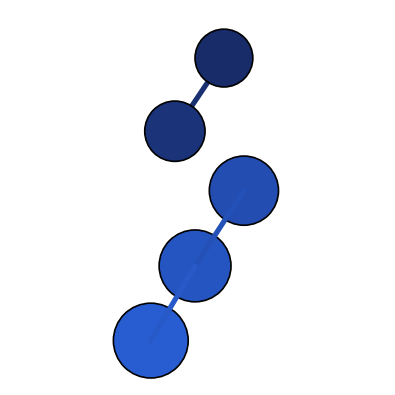
\includegraphics[width=0.8\linewidth]{figs/fragmented/N5_anion_anion_002_initial.png}\\[2pt]
{\small initiale (xTB, d\'ej\`a fragment\'ee, 2$+$3)}
\end{minipage}\hfill
\begin{minipage}{0.46\textwidth}
\centering
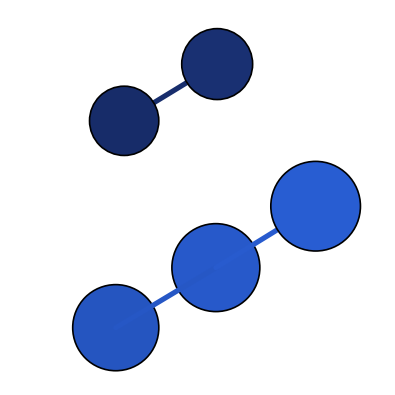
\includegraphics[width=0.8\linewidth]{figs/fragmented/N5_anion_anion_002_final.png}\\[2pt]
{\small DFT (fragment\'ee, 2$+$3)}
\end{minipage}
\end{figure}
\centerline{\small \texttt{N5\_anion\_anion\_002} -- fragments de taille 2$+$3}
\vspace{8pt}
\begin{figure}[H]
\centering
\begin{minipage}{0.46\textwidth}
\centering
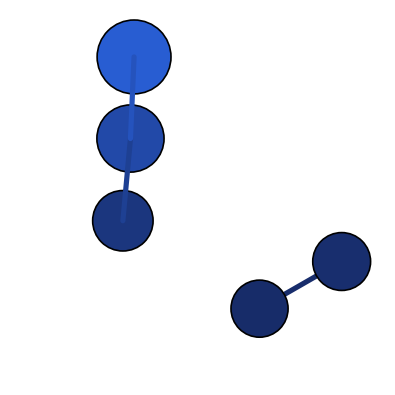
\includegraphics[width=0.8\linewidth]{figs/fragmented/N5_anion_anion_003_initial.png}\\[2pt]
{\small initiale (xTB, d\'ej\`a fragment\'ee, 2$+$3)}
\end{minipage}\hfill
\begin{minipage}{0.46\textwidth}
\centering
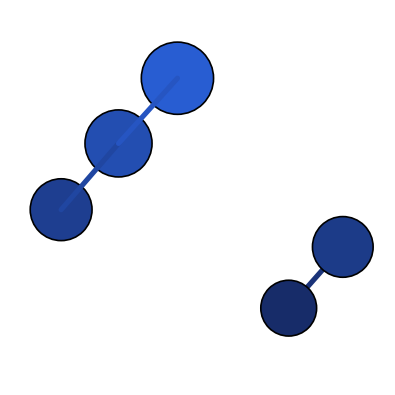
\includegraphics[width=0.8\linewidth]{figs/fragmented/N5_anion_anion_003_final.png}\\[2pt]
{\small DFT (fragment\'ee, 2$+$3)}
\end{minipage}
\end{figure}
\centerline{\small \texttt{N5\_anion\_anion\_003} -- fragments de taille 2$+$3}
\vspace{8pt}
\begin{figure}[H]
\centering
\begin{minipage}{0.46\textwidth}
\centering
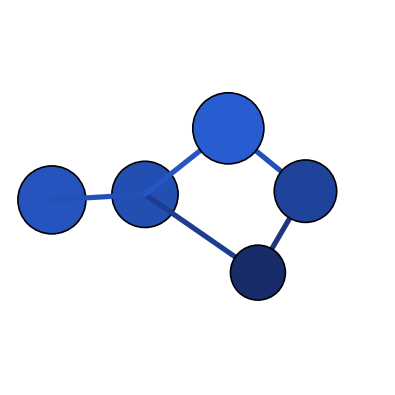
\includegraphics[width=0.8\linewidth]{figs/fragmented/N5_anion_anion_004_initial.png}\\[2pt]
{\small initiale (xTB, intacte, N$_5^{-}$)}
\end{minipage}\hfill
\begin{minipage}{0.46\textwidth}
\centering
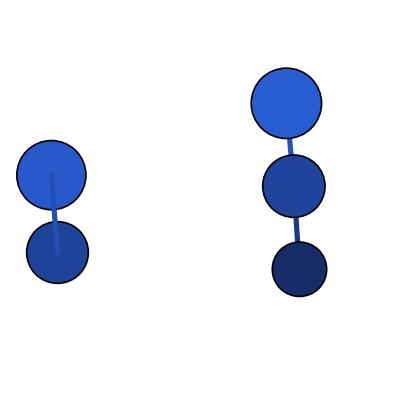
\includegraphics[width=0.8\linewidth]{figs/fragmented/N5_anion_anion_004_final.png}\\[2pt]
{\small DFT (fragment\'ee, 2$+$3)}
\end{minipage}
\end{figure}
\centerline{\small \texttt{N5\_anion\_anion\_004} -- fragments de taille 2$+$3}
\vspace{8pt}
\begin{figure}[H]
\centering
\begin{minipage}{0.46\textwidth}
\centering
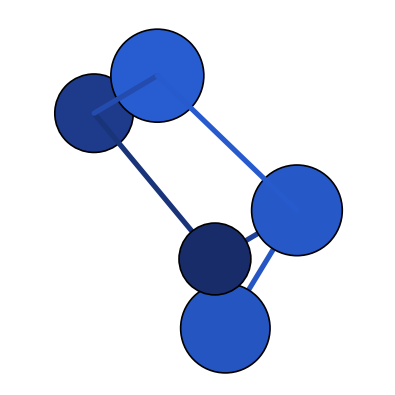
\includegraphics[width=0.8\linewidth]{figs/fragmented/N5_anion_anion_005_initial.png}\\[2pt]
{\small initiale (xTB, d\'ej\`a fragment\'ee, 2$+$3)}
\end{minipage}\hfill
\begin{minipage}{0.46\textwidth}
\centering
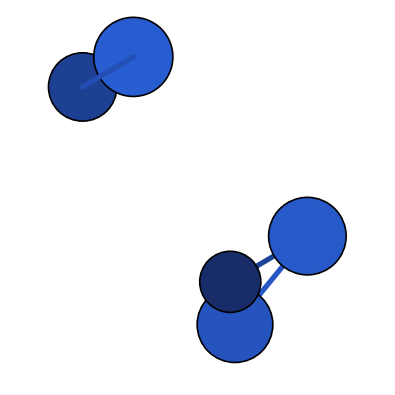
\includegraphics[width=0.8\linewidth]{figs/fragmented/N5_anion_anion_005_final.png}\\[2pt]
{\small DFT (fragment\'ee, 2$+$3)}
\end{minipage}
\end{figure}
\centerline{\small \texttt{N5\_anion\_anion\_005} -- fragments de taille 2$+$3}
\vspace{8pt}
\begin{figure}[H]
\centering
\begin{minipage}{0.46\textwidth}
\centering
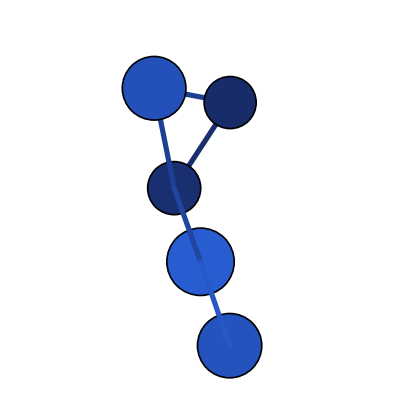
\includegraphics[width=0.8\linewidth]{figs/fragmented/N5_anion_anion_007_initial.png}\\[2pt]
{\small initiale (xTB, intacte, N$_5^{-}$)}
\end{minipage}\hfill
\begin{minipage}{0.46\textwidth}
\centering
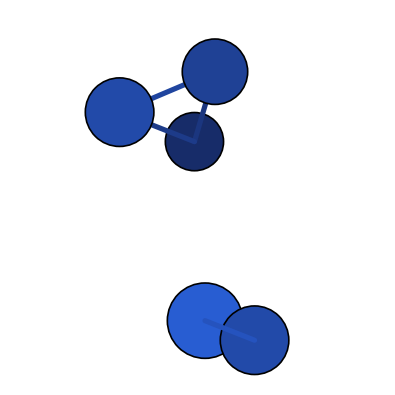
\includegraphics[width=0.8\linewidth]{figs/fragmented/N5_anion_anion_007_final.png}\\[2pt]
{\small DFT (fragment\'ee, 2$+$3)}
\end{minipage}
\end{figure}
\centerline{\small \texttt{N5\_anion\_anion\_007} -- fragments de taille 2$+$3}
\vspace{8pt}
\begin{figure}[H]
\centering
\begin{minipage}{0.46\textwidth}
\centering
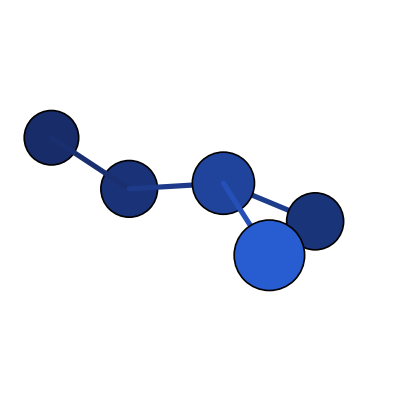
\includegraphics[width=0.8\linewidth]{figs/fragmented/N5_anion_anion_008_initial.png}\\[2pt]
{\small initiale (xTB, intacte, N$_5^{-}$)}
\end{minipage}\hfill
\begin{minipage}{0.46\textwidth}
\centering
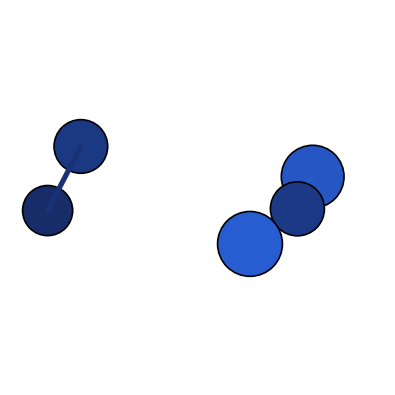
\includegraphics[width=0.8\linewidth]{figs/fragmented/N5_anion_anion_008_final.png}\\[2pt]
{\small DFT (fragment\'ee, 2$+$3)}
\end{minipage}
\end{figure}
\centerline{\small \texttt{N5\_anion\_anion\_008} -- fragments de taille 2$+$3}
\vspace{8pt}
\begin{figure}[H]
\centering
\begin{minipage}{0.46\textwidth}
\centering
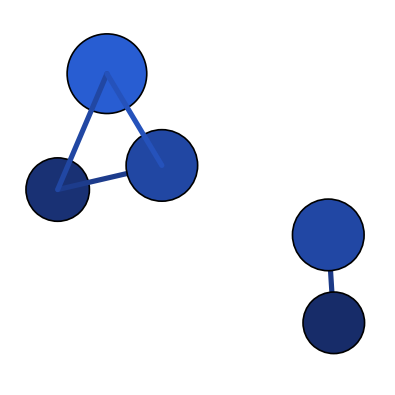
\includegraphics[width=0.8\linewidth]{figs/fragmented/N5_anion_anion_009_initial.png}\\[2pt]
{\small initiale (xTB, d\'ej\`a fragment\'ee, 2$+$3)}
\end{minipage}\hfill
\begin{minipage}{0.46\textwidth}
\centering
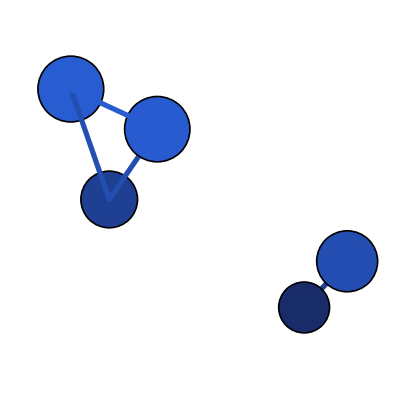
\includegraphics[width=0.8\linewidth]{figs/fragmented/N5_anion_anion_009_final.png}\\[2pt]
{\small DFT (fragment\'ee, 2$+$3)}
\end{minipage}
\end{figure}
\centerline{\small \texttt{N5\_anion\_anion\_009} -- fragments de taille 2$+$3}
\vspace{8pt}
\begin{figure}[H]
\centering
\begin{minipage}{0.46\textwidth}
\centering
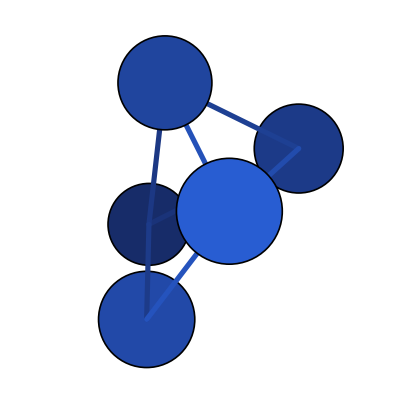
\includegraphics[width=0.8\linewidth]{figs/fragmented/N5_cation_cation_007_initial.png}\\[2pt]
{\small initiale (xTB, intacte, N$_5^{+}$)}
\end{minipage}\hfill
\begin{minipage}{0.46\textwidth}
\centering
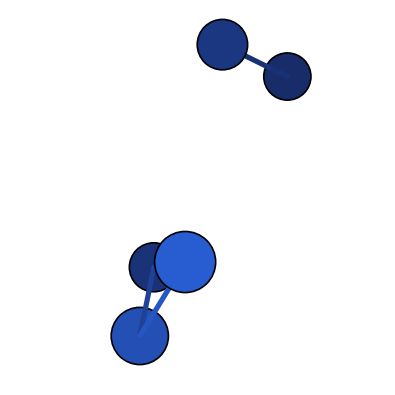
\includegraphics[width=0.8\linewidth]{figs/fragmented/N5_cation_cation_007_final.png}\\[2pt]
{\small DFT (fragment\'ee, 2$+$3)}
\end{minipage}
\end{figure}
\centerline{\small \texttt{N5\_cation\_cation\_007} -- fragments de taille 2$+$3}
\vspace{8pt}
\begin{figure}[H]
\centering
\begin{minipage}{0.46\textwidth}
\centering
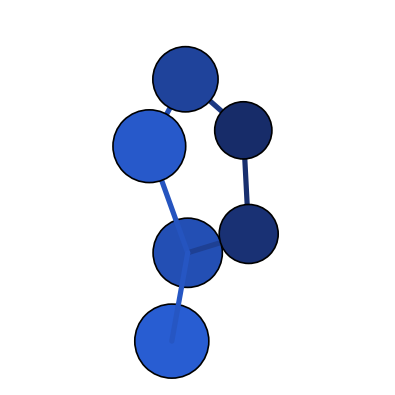
\includegraphics[width=0.8\linewidth]{figs/fragmented/N6_neutral_neutral_004_initial.png}\\[2pt]
{\small initiale (xTB, intacte, N$_6^{0}$)}
\end{minipage}\hfill
\begin{minipage}{0.46\textwidth}
\centering
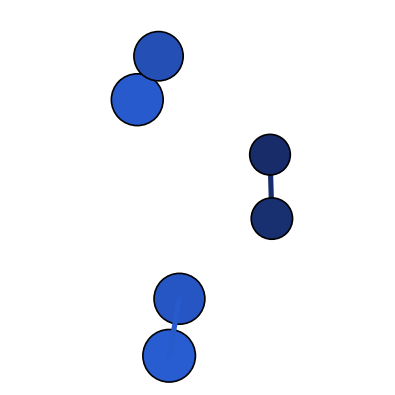
\includegraphics[width=0.8\linewidth]{figs/fragmented/N6_neutral_neutral_004_final.png}\\[2pt]
{\small DFT (fragment\'ee, 2$+$2$+$2)}
\end{minipage}
\end{figure}
\centerline{\small \texttt{N6\_neutral\_neutral\_004} -- fragments de taille 2$+$2$+$2}
\vspace{8pt}
\begin{figure}[H]
\centering
\begin{minipage}{0.46\textwidth}
\centering
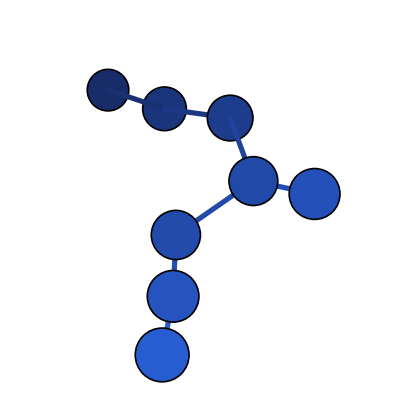
\includegraphics[width=0.8\linewidth]{figs/fragmented/N8_neutral_neutral_006_initial.png}\\[2pt]
{\small initiale (xTB, intacte, N$_8^{0}$)}
\end{minipage}\hfill
\begin{minipage}{0.46\textwidth}
\centering
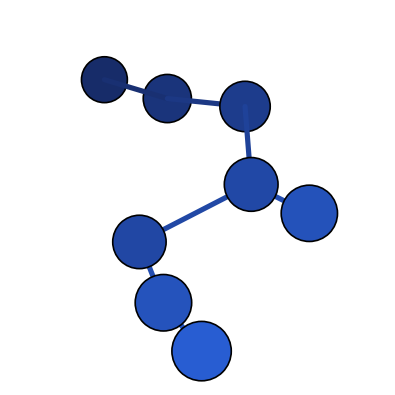
\includegraphics[width=0.8\linewidth]{figs/fragmented/N8_neutral_neutral_006_final.png}\\[2pt]
{\small DFT (fragment\'ee, 3$+$5)}
\end{minipage}
\end{figure}
\centerline{\small \texttt{N8\_neutral\_neutral\_006} -- fragments de taille 3$+$5}
\vspace{8pt}
\begin{figure}[H]
\centering
\begin{minipage}{0.46\textwidth}
\centering
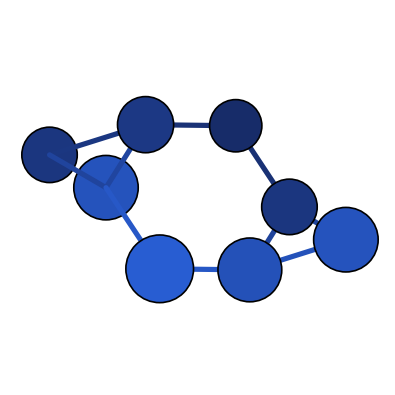
\includegraphics[width=0.8\linewidth]{figs/fragmented/N8_neutral_neutral_018_initial.png}\\[2pt]
{\small initiale (xTB, intacte, N$_8^{0}$)}
\end{minipage}\hfill
\begin{minipage}{0.46\textwidth}
\centering
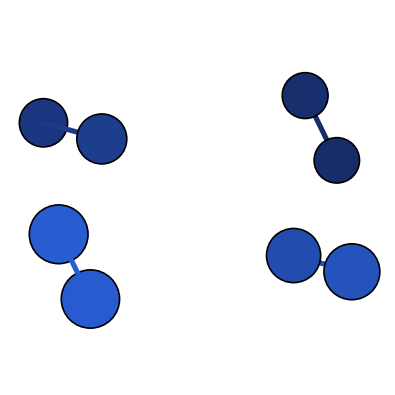
\includegraphics[width=0.8\linewidth]{figs/fragmented/N8_neutral_neutral_018_final.png}\\[2pt]
{\small DFT (fragment\'ee, 2$+$2$+$2$+$2)}
\end{minipage}
\end{figure}
\centerline{\small \texttt{N8\_neutral\_neutral\_018} -- fragments de taille 2$+$2$+$2$+$2}
\vspace{8pt}
\begin{figure}[H]
\centering
\begin{minipage}{0.46\textwidth}
\centering
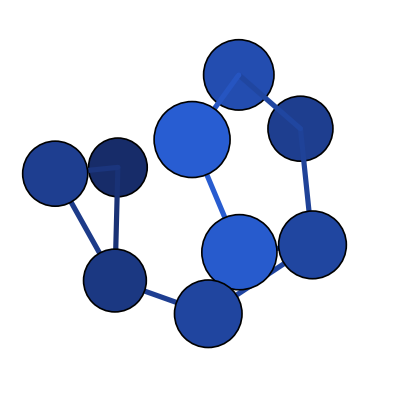
\includegraphics[width=0.8\linewidth]{figs/fragmented/N9_anion_anion_015_initial.png}\\[2pt]
{\small initiale (xTB, intacte, N$_9^{-}$)}
\end{minipage}\hfill
\begin{minipage}{0.46\textwidth}
\centering
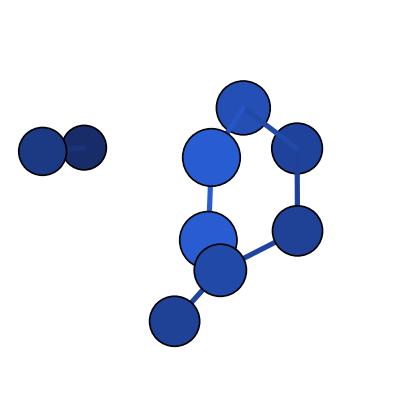
\includegraphics[width=0.8\linewidth]{figs/fragmented/N9_anion_anion_015_final.png}\\[2pt]
{\small DFT (fragment\'ee, 2$+$7)}
\end{minipage}
\end{figure}
\centerline{\small \texttt{N9\_anion\_anion\_015} -- fragments de taille 2$+$7}
\vspace{8pt}
\begin{figure}[H]
\centering
\begin{minipage}{0.46\textwidth}
\centering
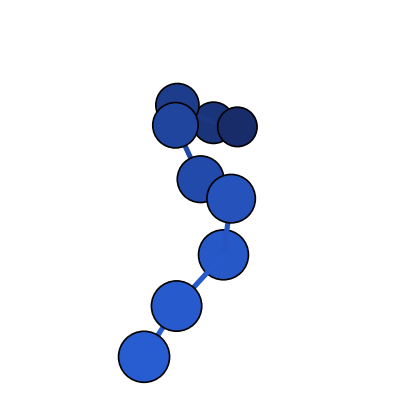
\includegraphics[width=0.8\linewidth]{figs/fragmented/N9_cation_cation_001_initial.png}\\[2pt]
{\small initiale (xTB, intacte, N$_9^{+}$)}
\end{minipage}\hfill
\begin{minipage}{0.46\textwidth}
\centering
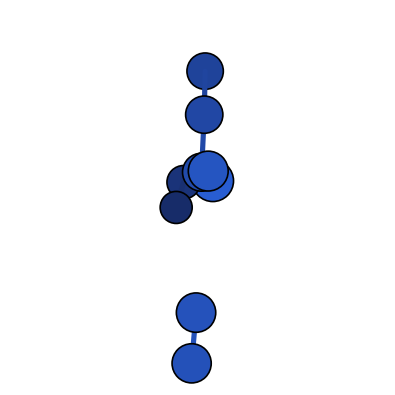
\includegraphics[width=0.8\linewidth]{figs/fragmented/N9_cation_cation_001_final.png}\\[2pt]
{\small DFT (fragment\'ee, 2$+$2$+$5)}
\end{minipage}
\end{figure}
\centerline{\small \texttt{N9\_cation\_cation\_001} -- fragments de taille 2$+$2$+$5}
\vspace{8pt}
\begin{figure}[H]
\centering
\begin{minipage}{0.46\textwidth}
\centering
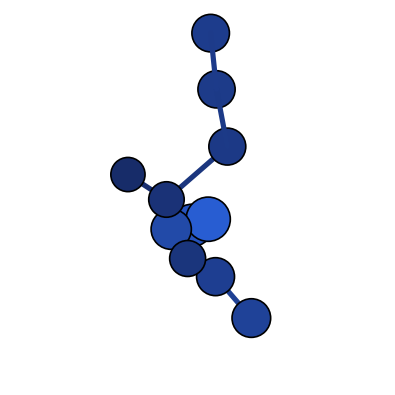
\includegraphics[width=0.8\linewidth]{figs/fragmented/N11_anion_anion_011_initial.png}\\[2pt]
{\small initiale (xTB, d\'ej\`a fragment\'ee, 3$+$3$+$5)}
\end{minipage}\hfill
\begin{minipage}{0.46\textwidth}
\centering
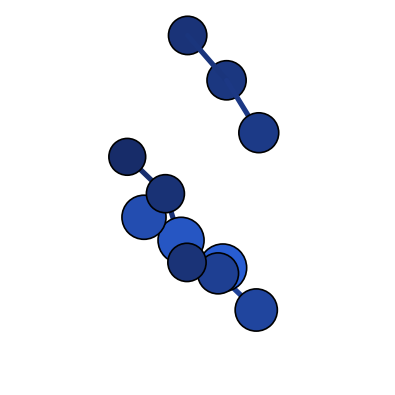
\includegraphics[width=0.8\linewidth]{figs/fragmented/N11_anion_anion_011_final.png}\\[2pt]
{\small DFT (fragment\'ee, 3$+$3$+$5)}
\end{minipage}
\end{figure}
\centerline{\small \texttt{N11\_anion\_anion\_011} -- fragments de taille 3$+$3$+$5}
\vspace{8pt}
\begin{figure}[H]
\centering
\begin{minipage}{0.46\textwidth}
\centering
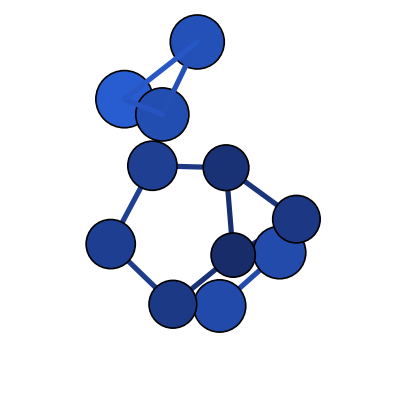
\includegraphics[width=0.8\linewidth]{figs/fragmented/N11_anion_anion_018_initial.png}\\[2pt]
{\small initiale (xTB, intacte, N$_11^{-}$)}
\end{minipage}\hfill
\begin{minipage}{0.46\textwidth}
\centering
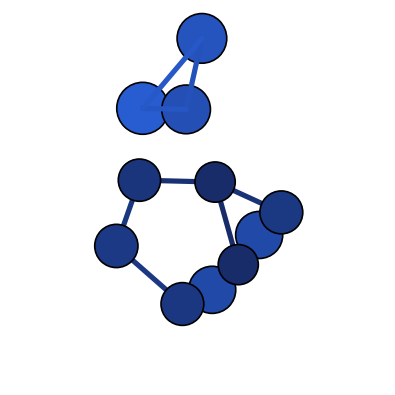
\includegraphics[width=0.8\linewidth]{figs/fragmented/N11_anion_anion_018_final.png}\\[2pt]
{\small DFT (fragment\'ee, 3$+$8)}
\end{minipage}
\end{figure}
\centerline{\small \texttt{N11\_anion\_anion\_018} -- fragments de taille 3$+$8}
\vspace{8pt}
\begin{figure}[H]
\centering
\begin{minipage}{0.46\textwidth}
\centering
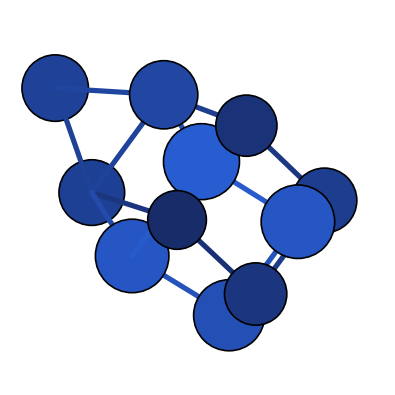
\includegraphics[width=0.8\linewidth]{figs/fragmented/N11_cation_cation_009_initial.png}\\[2pt]
{\small initiale (xTB, intacte, N$_11^{+}$)}
\end{minipage}\hfill
\begin{minipage}{0.46\textwidth}
\centering
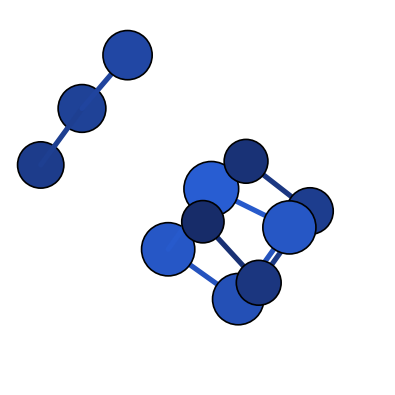
\includegraphics[width=0.8\linewidth]{figs/fragmented/N11_cation_cation_009_final.png}\\[2pt]
{\small DFT (fragment\'ee, 3$+$8)}
\end{minipage}
\end{figure}
\centerline{\small \texttt{N11\_cation\_cation\_009} -- fragments de taille 3$+$8}
\vspace{8pt}
\begin{figure}[H]
\centering
\begin{minipage}{0.46\textwidth}
\centering
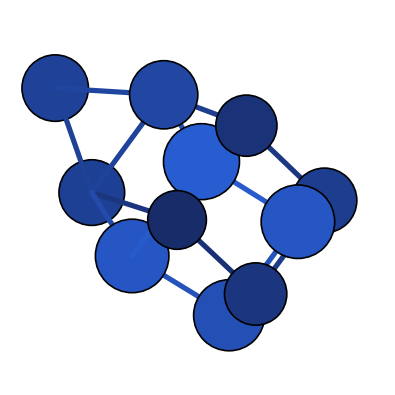
\includegraphics[width=0.8\linewidth]{figs/fragmented/N11_cation_cation_010_initial.png}\\[2pt]
{\small initiale (xTB, intacte, N$_11^{+}$)}
\end{minipage}\hfill
\begin{minipage}{0.46\textwidth}
\centering
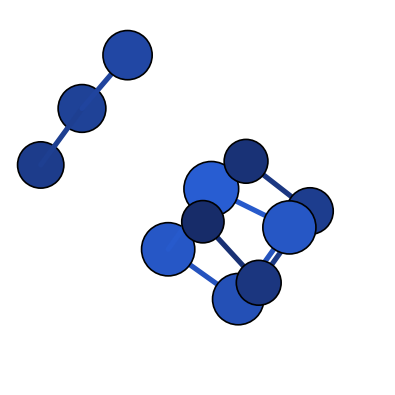
\includegraphics[width=0.8\linewidth]{figs/fragmented/N11_cation_cation_010_final.png}\\[2pt]
{\small DFT (fragment\'ee, 3$+$8)}
\end{minipage}
\end{figure}
\centerline{\small \texttt{N11\_cation\_cation\_010} -- fragments de taille 3$+$8}
\vspace{8pt}
\begin{figure}[H]
\centering
\begin{minipage}{0.46\textwidth}
\centering
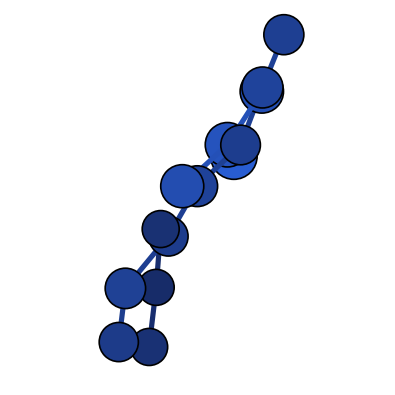
\includegraphics[width=0.8\linewidth]{figs/fragmented/N14_neutral_neutral_004_initial.png}\\[2pt]
{\small initiale (xTB, intacte, N$_14^{0}$)}
\end{minipage}\hfill
\begin{minipage}{0.46\textwidth}
\centering
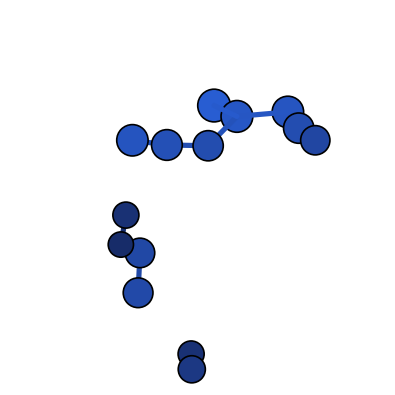
\includegraphics[width=0.8\linewidth]{figs/fragmented/N14_neutral_neutral_004_final.png}\\[2pt]
{\small DFT (fragment\'ee, 2$+$2$+$2$+$3$+$5)}
\end{minipage}
\end{figure}
\centerline{\small \texttt{N14\_neutral\_neutral\_004} -- fragments de taille 2$+$2$+$2$+$3$+$5}
\vspace{8pt}
\bigskip\noindent\textit{L\'egende g\'en\'erale, Figure~S1~:} sph\`eres bleues reli\'ees par des b\^atonnets = atomes N et liaisons N--N (mod\`ele boules-b\^atonnets, rendu depuis les coordonn\'ees cart\'esiennes .xyz) ; paires group\'ees par candidat, g\'eom\'etrie initiale GFN2-xTB \`a gauche et g\'eom\'etrie finale DFT WB97X-D4 \`a droite pour chacun des 18 candidats fragment\'es dont le calcul DFT est termin\'e (sur les 24 recens\'es au Tableau~S1 ; les autres n'ont pas encore de g\'eom\'etrie DFT \`a montrer).

\subsection{Structures non convergées}
\label{sec:si-nonconverged}

\noindent\textbf{Tableau S2.} Structures dont l'optimisation g\'eom\'etrique DFT WB97X-D4/aug-cc-pVTZ n'a \textbf{pas converg\'e} -- l'optimiseur a atteint sa limite de 50 cycles (\texttt{The optimization did not converge but reached the maximum}) sans trouver de point stationnaire. \'Energie non fiable, structures exclues de tous les tableaux d'analyse (\S\ref{sec:provenance}--\ref{sec:bonds}) et de la comparaison de stabilit\'e (\S\ref{sec:litterature}) tant qu'elles n'ont pas \'et\'e reprises. \textbf{28~des 35~n'ont en r\'ealit\'e probablement jamais de minimum li\'e} : la colonne \emph{Frag.\ dernier cycle} montre qu'elles sont d\'ej\`a s\'epar\'ees en plusieurs composantes connexes (seuil 1,70~\AA) \`a la derni\`ere g\'eom\'etrie tent\'ee -- l'optimiseur suit un gradient de dissociation qui ne s'annule jamais en un nombre fini de cycles, plut\^ot qu'un probl\`eme num\'erique de convergence~; les relancer avec \texttt{\%geom MaxIter} plus grand ne changera probablement rien. Seules les 7 restantes (compos\'e li\'e unique au dernier cycle) sont des candidates cr\'edibles \`a une reprise avec davantage de cycles. Repr\'esentations avant/dernier cycle en Figure~S2.\par\vspace{4pt}
{\scriptsize
\begin{longtable}{@{}p{3.8cm}ccrp{1.6cm}c@{}}
\label{tab:nonconverged}\\
\toprule
\textbf{Nom} & \textbf{N} & \textbf{Charge} & \textbf{Cycles} & \textbf{Frag.\ dernier cycle} & \textbf{R\'ef.} \\
\midrule\endfirsthead
\multicolumn{6}{c}{\small (suite)}\\ \toprule\endhead
\bottomrule\endfoot
\bottomrule\endlastfoot
\texttt{N6\_neutral\_neutral\_011} & 6 & 0 & 50 & \checkmark~(2$+$4) & our work \\
\texttt{N7\_anion\_anion\_006} & 7 & - & 50 & \checkmark~(2$+$2$+$3) & our work \\
\texttt{N7\_anion\_anion\_015} & 7 & - & 50 & \checkmark~(2$+$2$+$3) & our work \\
\texttt{N7\_cation\_cation\_002} & 7 & + & 50 & \checkmark~(2$+$5) & our work \\
\texttt{N7\_cation\_cation\_004} & 7 & + & 50 & \checkmark~(2$+$2$+$3) & our work \\
\texttt{N8\_neutral\_neutral\_011} & 8 & 0 & 50 & non & our work \\
\texttt{N8\_neutral\_neutral\_015} & 8 & 0 & 50 & non & our work \\
\texttt{N8\_neutral\_neutral\_017} & 8 & 0 & 50 & \checkmark~(2$+$6) & our work \\
\texttt{N9\_anion\_anion\_002} & 9 & - & 50 & \checkmark~(2$+$2$+$5) & our work \\
\texttt{N9\_anion\_anion\_007} & 9 & - & 50 & \checkmark~(3$+$6) & our work \\
\texttt{N9\_anion\_anion\_009} & 9 & - & 50 & \checkmark~(2$+$7) & our work \\
\texttt{N9\_anion\_anion\_014} & 9 & - & 50 & \checkmark~(2$+$7) & our work \\
\texttt{N9\_anion\_anion\_017} & 9 & - & 50 & non & our work \\
\texttt{N9\_anion\_anion\_020} & 9 & - & 50 & \checkmark~(2$+$7) & our work \\
\texttt{N9\_cation\_cation\_002} & 9 & + & 50 & \checkmark~(2$+$2$+$5) & our work \\
\texttt{N9\_cation\_cation\_003} & 9 & + & 50 & \checkmark~(2$+$7) & our work \\
\texttt{N9\_cation\_cation\_004} & 9 & + & 50 & \checkmark~(2$+$2$+$5) & our work \\
\texttt{N9\_cation\_cation\_005} & 9 & + & 50 & \checkmark~(2$+$2$+$2$+$3) & our work \\
\texttt{N9\_cation\_cation\_007} & 9 & + & 50 & \checkmark~(2$+$2$+$5) & our work \\
\texttt{N9\_cation\_cation\_010} & 9 & + & 50 & non & our work \\
\texttt{N10\_neutral\_neutral\_008} & 10 & 0 & 50 & \checkmark~(2$+$2$+$3$+$3) & our work \\
\texttt{N10\_neutral\_neutral\_009} & 10 & 0 & 50 & \checkmark~(2$+$8) & our work \\
\texttt{N10\_neutral\_neutral\_012} & 10 & 0 & 50 & \checkmark~(2$+$2$+$6) & our work \\
\texttt{N11\_anion\_anion\_009} & 11 & - & 50 & \checkmark~(2$+$2$+$7) & our work \\
\texttt{N11\_anion\_anion\_012} & 11 & - & 50 & non & our work \\
\texttt{N11\_anion\_anion\_014} & 11 & - & 50 & \checkmark~(2$+$9) & our work \\
\texttt{N11\_anion\_anion\_015} & 11 & - & 50 & non & our work \\
\texttt{N11\_anion\_anion\_016} & 11 & - & 50 & \checkmark~(2$+$2$+$7) & our work \\
\texttt{N11\_cation\_cation\_003} & 11 & + & 50 & \checkmark~(2$+$2$+$7) & our work \\
\texttt{N11\_cation\_cation\_008} & 11 & + & 50 & \checkmark~(2$+$2$+$2$+$5) & our work \\
\texttt{N13\_anion\_anion\_002} & 13 & - & 50 & \checkmark~(2$+$11) & our work \\
\texttt{N13\_anion\_anion\_003} & 13 & - & 50 & non & our work \\
\texttt{N13\_anion\_anion\_004} & 13 & - & 50 & \checkmark~(2$+$11) & our work \\
\texttt{N13\_cation\_cation\_002} & 13 & + & 50 & \checkmark~(2$+$2$+$2$+$7) & our work \\
\texttt{N13\_cation\_cation\_003} & 13 & + & 50 & \checkmark~(2$+$2$+$9) & our work \\
\end{longtable}
}

\bigskip
\subsection*{Figure S2 -- structures non convergées (avant / dernier cycle)}
Pour chaque candidat non converg\'e (Tableau~S2)~: \`a gauche la g\'eom\'etrie initiale (criblage GFN2-xTB), \`a droite la derni\`ere g\'eom\'etrie tent\'ee par l'optimiseur DFT avant d'atteindre la limite de cycles -- pas un minimum, juste le dernier point de la trajectoire d'optimisation.
\begin{figure}[H]
\centering
\begin{minipage}{0.46\textwidth}
\centering
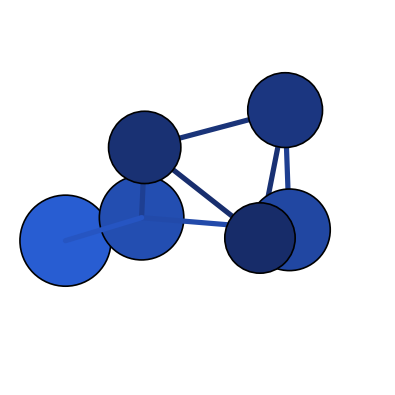
\includegraphics[width=0.8\linewidth]{figs/nonconverged/N6_neutral_neutral_011_initial.png}\\[2pt]
{\small initiale (xTB, N$_6^{0}$)}
\end{minipage}\hfill
\begin{minipage}{0.46\textwidth}
\centering
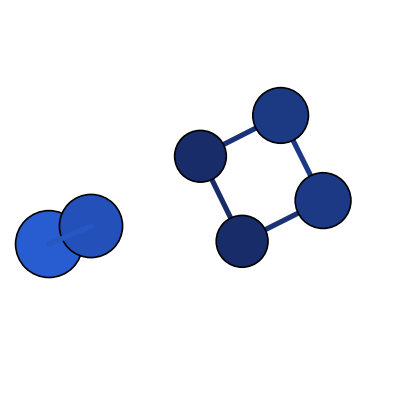
\includegraphics[width=0.8\linewidth]{figs/nonconverged/N6_neutral_neutral_011_last.png}\\[2pt]
{\small dernier cycle DFT (50 cycles)}
\end{minipage}
\end{figure}
\centerline{\small \texttt{N6\_neutral\_neutral\_011} -- en cours de fragmentation, 2$+$4}
\vspace{8pt}
\begin{figure}[H]
\centering
\begin{minipage}{0.46\textwidth}
\centering
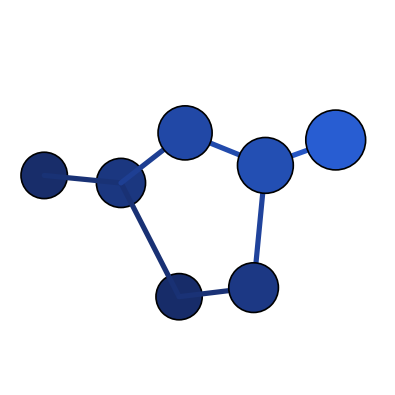
\includegraphics[width=0.8\linewidth]{figs/nonconverged/N7_anion_anion_006_initial.png}\\[2pt]
{\small initiale (xTB, N$_7^{-}$)}
\end{minipage}\hfill
\begin{minipage}{0.46\textwidth}
\centering
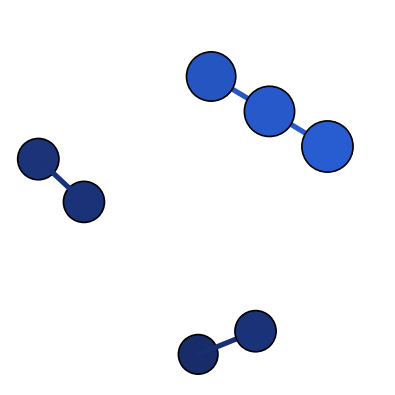
\includegraphics[width=0.8\linewidth]{figs/nonconverged/N7_anion_anion_006_last.png}\\[2pt]
{\small dernier cycle DFT (50 cycles)}
\end{minipage}
\end{figure}
\centerline{\small \texttt{N7\_anion\_anion\_006} -- en cours de fragmentation, 2$+$2$+$3}
\vspace{8pt}
\begin{figure}[H]
\centering
\begin{minipage}{0.46\textwidth}
\centering
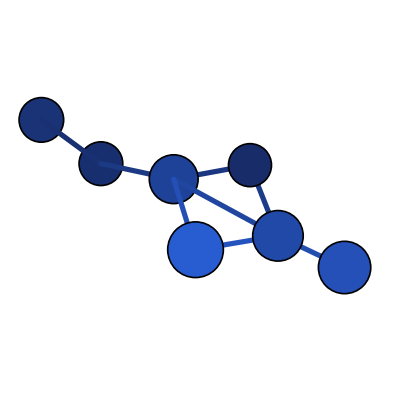
\includegraphics[width=0.8\linewidth]{figs/nonconverged/N7_anion_anion_015_initial.png}\\[2pt]
{\small initiale (xTB, N$_7^{-}$)}
\end{minipage}\hfill
\begin{minipage}{0.46\textwidth}
\centering
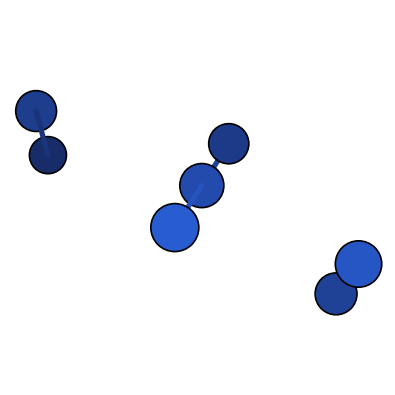
\includegraphics[width=0.8\linewidth]{figs/nonconverged/N7_anion_anion_015_last.png}\\[2pt]
{\small dernier cycle DFT (50 cycles)}
\end{minipage}
\end{figure}
\centerline{\small \texttt{N7\_anion\_anion\_015} -- en cours de fragmentation, 2$+$2$+$3}
\vspace{8pt}
\begin{figure}[H]
\centering
\begin{minipage}{0.46\textwidth}
\centering
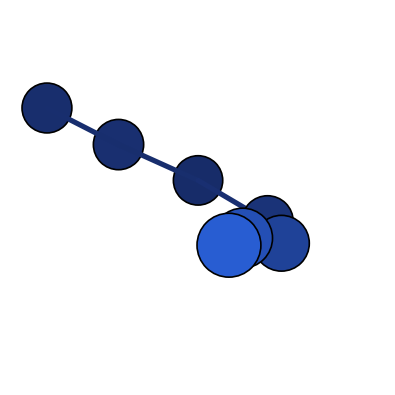
\includegraphics[width=0.8\linewidth]{figs/nonconverged/N7_cation_cation_002_initial.png}\\[2pt]
{\small initiale (xTB, N$_7^{+}$)}
\end{minipage}\hfill
\begin{minipage}{0.46\textwidth}
\centering
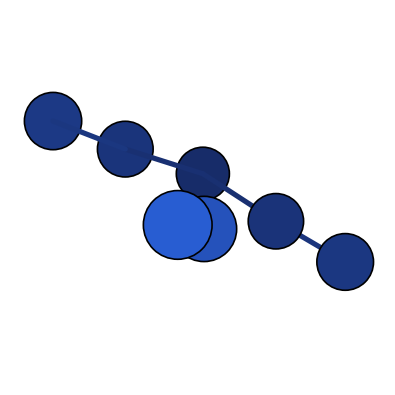
\includegraphics[width=0.8\linewidth]{figs/nonconverged/N7_cation_cation_002_last.png}\\[2pt]
{\small dernier cycle DFT (50 cycles)}
\end{minipage}
\end{figure}
\centerline{\small \texttt{N7\_cation\_cation\_002} -- en cours de fragmentation, 2$+$5}
\vspace{8pt}
\begin{figure}[H]
\centering
\begin{minipage}{0.46\textwidth}
\centering
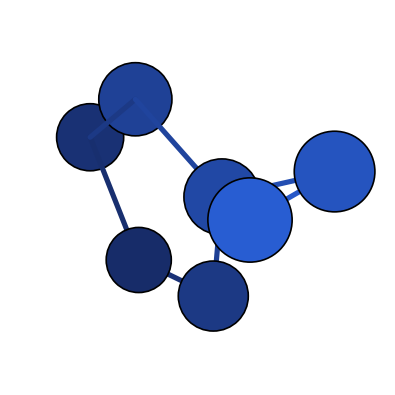
\includegraphics[width=0.8\linewidth]{figs/nonconverged/N7_cation_cation_004_initial.png}\\[2pt]
{\small initiale (xTB, N$_7^{+}$)}
\end{minipage}\hfill
\begin{minipage}{0.46\textwidth}
\centering
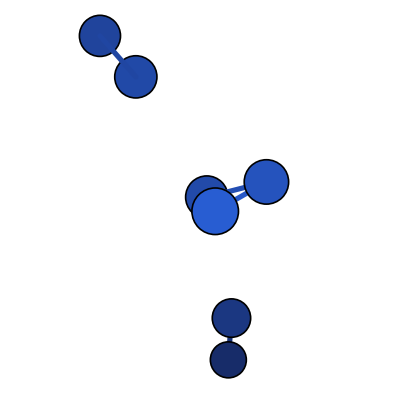
\includegraphics[width=0.8\linewidth]{figs/nonconverged/N7_cation_cation_004_last.png}\\[2pt]
{\small dernier cycle DFT (50 cycles)}
\end{minipage}
\end{figure}
\centerline{\small \texttt{N7\_cation\_cation\_004} -- en cours de fragmentation, 2$+$2$+$3}
\vspace{8pt}
\begin{figure}[H]
\centering
\begin{minipage}{0.46\textwidth}
\centering
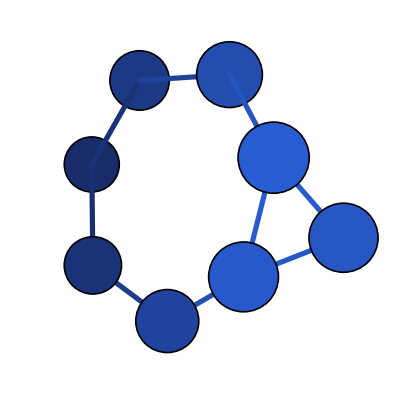
\includegraphics[width=0.8\linewidth]{figs/nonconverged/N8_neutral_neutral_011_initial.png}\\[2pt]
{\small initiale (xTB, N$_8^{0}$)}
\end{minipage}\hfill
\begin{minipage}{0.46\textwidth}
\centering
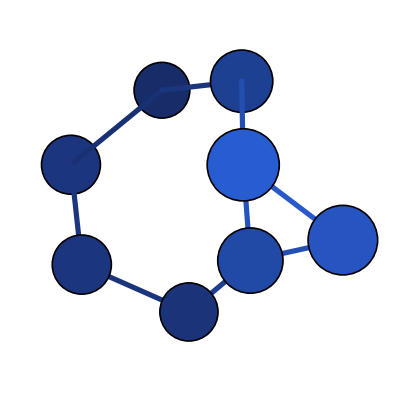
\includegraphics[width=0.8\linewidth]{figs/nonconverged/N8_neutral_neutral_011_last.png}\\[2pt]
{\small dernier cycle DFT (50 cycles)}
\end{minipage}
\end{figure}
\centerline{\small \texttt{N8\_neutral\_neutral\_011} -- cluster unique -- non-convergence num\'erique}
\vspace{8pt}
\begin{figure}[H]
\centering
\begin{minipage}{0.46\textwidth}
\centering
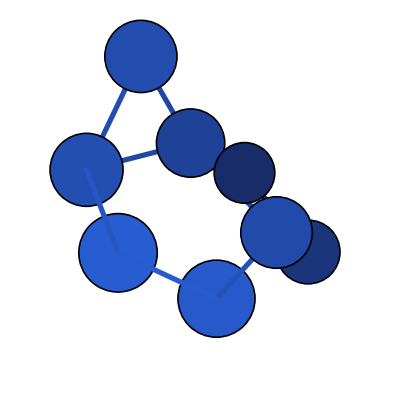
\includegraphics[width=0.8\linewidth]{figs/nonconverged/N8_neutral_neutral_015_initial.png}\\[2pt]
{\small initiale (xTB, N$_8^{0}$)}
\end{minipage}\hfill
\begin{minipage}{0.46\textwidth}
\centering
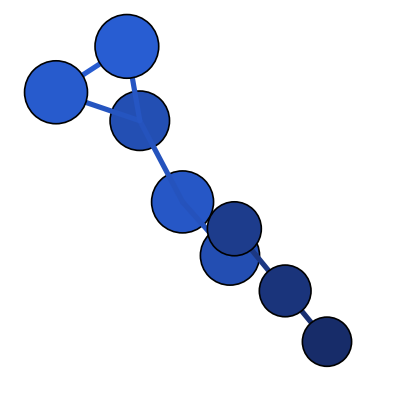
\includegraphics[width=0.8\linewidth]{figs/nonconverged/N8_neutral_neutral_015_last.png}\\[2pt]
{\small dernier cycle DFT (50 cycles)}
\end{minipage}
\end{figure}
\centerline{\small \texttt{N8\_neutral\_neutral\_015} -- cluster unique -- non-convergence num\'erique}
\vspace{8pt}
\begin{figure}[H]
\centering
\begin{minipage}{0.46\textwidth}
\centering
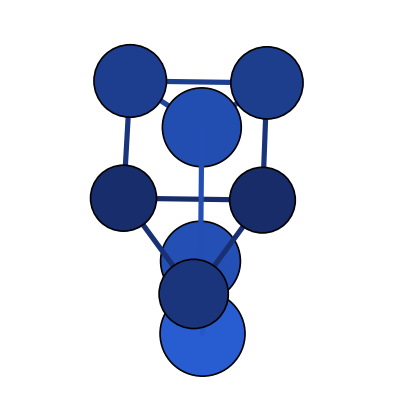
\includegraphics[width=0.8\linewidth]{figs/nonconverged/N8_neutral_neutral_017_initial.png}\\[2pt]
{\small initiale (xTB, N$_8^{0}$)}
\end{minipage}\hfill
\begin{minipage}{0.46\textwidth}
\centering
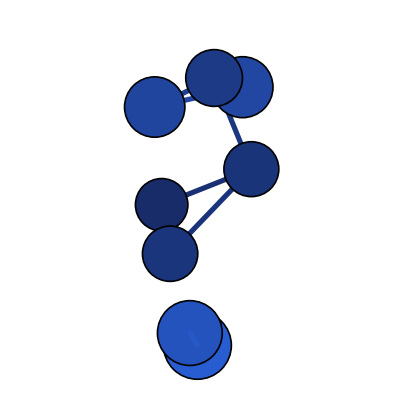
\includegraphics[width=0.8\linewidth]{figs/nonconverged/N8_neutral_neutral_017_last.png}\\[2pt]
{\small dernier cycle DFT (50 cycles)}
\end{minipage}
\end{figure}
\centerline{\small \texttt{N8\_neutral\_neutral\_017} -- en cours de fragmentation, 2$+$6}
\vspace{8pt}
\begin{figure}[H]
\centering
\begin{minipage}{0.46\textwidth}
\centering
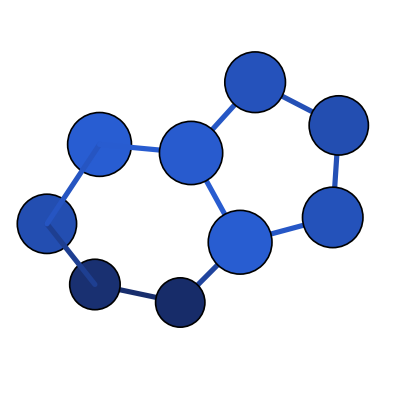
\includegraphics[width=0.8\linewidth]{figs/nonconverged/N9_anion_anion_002_initial.png}\\[2pt]
{\small initiale (xTB, N$_9^{-}$)}
\end{minipage}\hfill
\begin{minipage}{0.46\textwidth}
\centering
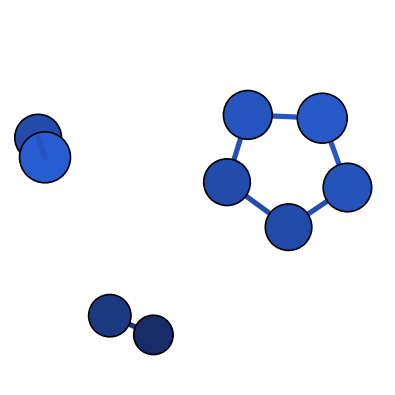
\includegraphics[width=0.8\linewidth]{figs/nonconverged/N9_anion_anion_002_last.png}\\[2pt]
{\small dernier cycle DFT (50 cycles)}
\end{minipage}
\end{figure}
\centerline{\small \texttt{N9\_anion\_anion\_002} -- en cours de fragmentation, 2$+$2$+$5}
\vspace{8pt}
\begin{figure}[H]
\centering
\begin{minipage}{0.46\textwidth}
\centering
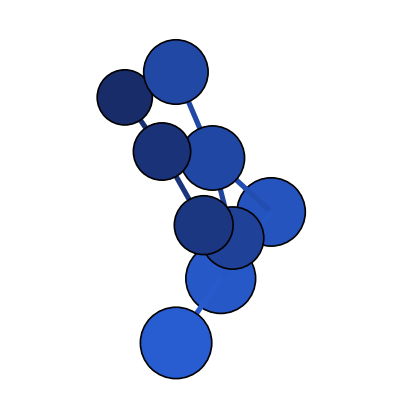
\includegraphics[width=0.8\linewidth]{figs/nonconverged/N9_anion_anion_007_initial.png}\\[2pt]
{\small initiale (xTB, N$_9^{-}$)}
\end{minipage}\hfill
\begin{minipage}{0.46\textwidth}
\centering
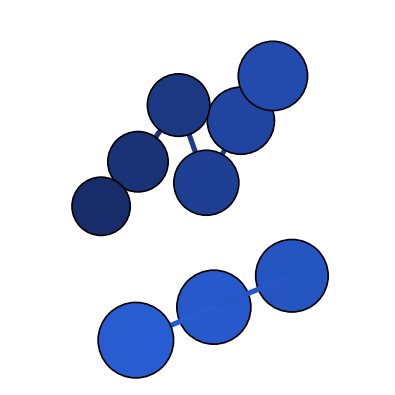
\includegraphics[width=0.8\linewidth]{figs/nonconverged/N9_anion_anion_007_last.png}\\[2pt]
{\small dernier cycle DFT (50 cycles)}
\end{minipage}
\end{figure}
\centerline{\small \texttt{N9\_anion\_anion\_007} -- en cours de fragmentation, 3$+$6}
\vspace{8pt}
\begin{figure}[H]
\centering
\begin{minipage}{0.46\textwidth}
\centering
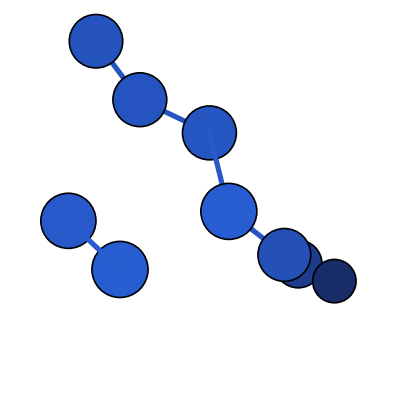
\includegraphics[width=0.8\linewidth]{figs/nonconverged/N9_anion_anion_009_initial.png}\\[2pt]
{\small initiale (xTB, N$_9^{-}$)}
\end{minipage}\hfill
\begin{minipage}{0.46\textwidth}
\centering
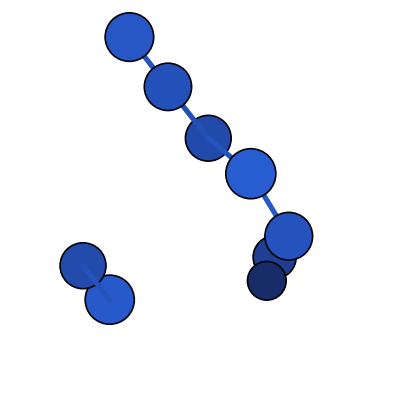
\includegraphics[width=0.8\linewidth]{figs/nonconverged/N9_anion_anion_009_last.png}\\[2pt]
{\small dernier cycle DFT (50 cycles)}
\end{minipage}
\end{figure}
\centerline{\small \texttt{N9\_anion\_anion\_009} -- en cours de fragmentation, 2$+$7}
\vspace{8pt}
\begin{figure}[H]
\centering
\begin{minipage}{0.46\textwidth}
\centering
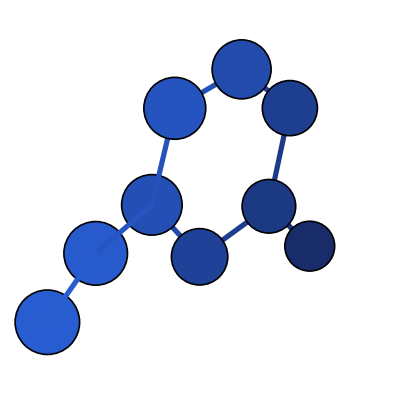
\includegraphics[width=0.8\linewidth]{figs/nonconverged/N9_anion_anion_014_initial.png}\\[2pt]
{\small initiale (xTB, N$_9^{-}$)}
\end{minipage}\hfill
\begin{minipage}{0.46\textwidth}
\centering
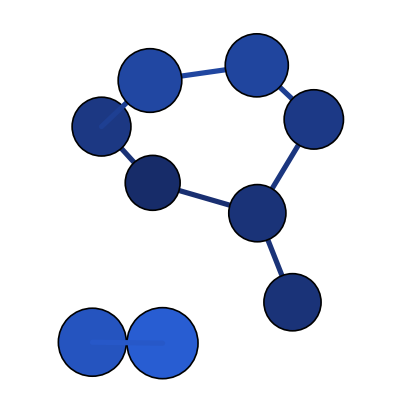
\includegraphics[width=0.8\linewidth]{figs/nonconverged/N9_anion_anion_014_last.png}\\[2pt]
{\small dernier cycle DFT (50 cycles)}
\end{minipage}
\end{figure}
\centerline{\small \texttt{N9\_anion\_anion\_014} -- en cours de fragmentation, 2$+$7}
\vspace{8pt}
\begin{figure}[H]
\centering
\begin{minipage}{0.46\textwidth}
\centering
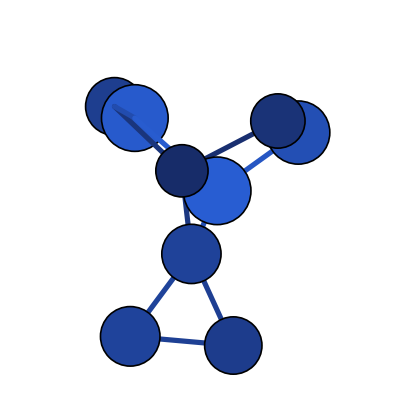
\includegraphics[width=0.8\linewidth]{figs/nonconverged/N9_anion_anion_017_initial.png}\\[2pt]
{\small initiale (xTB, N$_9^{-}$)}
\end{minipage}\hfill
\begin{minipage}{0.46\textwidth}
\centering
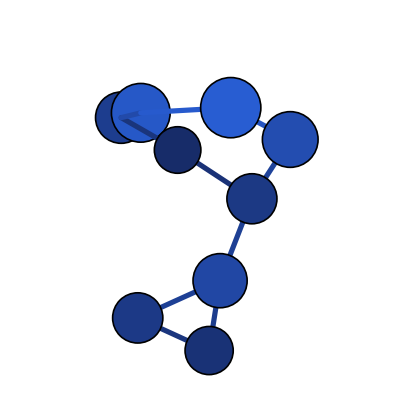
\includegraphics[width=0.8\linewidth]{figs/nonconverged/N9_anion_anion_017_last.png}\\[2pt]
{\small dernier cycle DFT (50 cycles)}
\end{minipage}
\end{figure}
\centerline{\small \texttt{N9\_anion\_anion\_017} -- cluster unique -- non-convergence num\'erique}
\vspace{8pt}
\begin{figure}[H]
\centering
\begin{minipage}{0.46\textwidth}
\centering
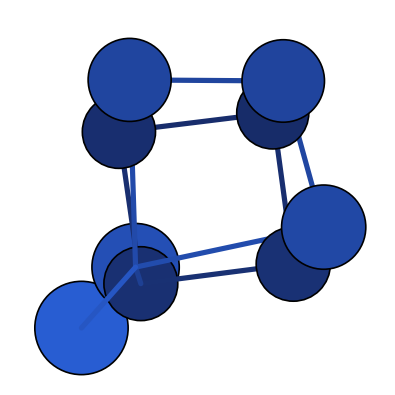
\includegraphics[width=0.8\linewidth]{figs/nonconverged/N9_anion_anion_020_initial.png}\\[2pt]
{\small initiale (xTB, N$_9^{-}$)}
\end{minipage}\hfill
\begin{minipage}{0.46\textwidth}
\centering
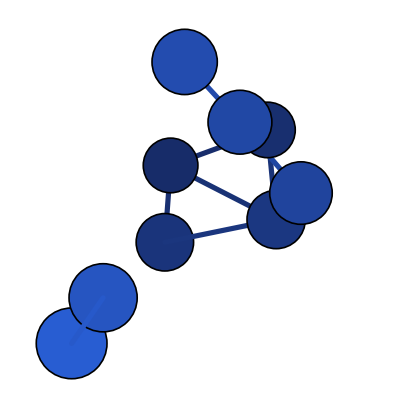
\includegraphics[width=0.8\linewidth]{figs/nonconverged/N9_anion_anion_020_last.png}\\[2pt]
{\small dernier cycle DFT (50 cycles)}
\end{minipage}
\end{figure}
\centerline{\small \texttt{N9\_anion\_anion\_020} -- en cours de fragmentation, 2$+$7}
\vspace{8pt}
\begin{figure}[H]
\centering
\begin{minipage}{0.46\textwidth}
\centering
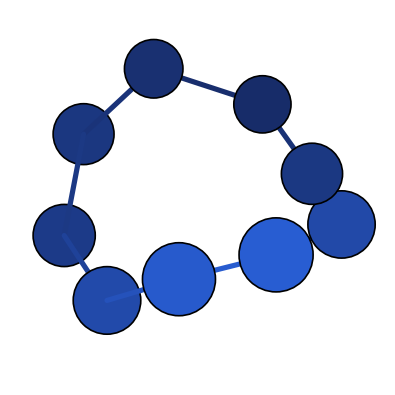
\includegraphics[width=0.8\linewidth]{figs/nonconverged/N9_cation_cation_002_initial.png}\\[2pt]
{\small initiale (xTB, N$_9^{+}$)}
\end{minipage}\hfill
\begin{minipage}{0.46\textwidth}
\centering
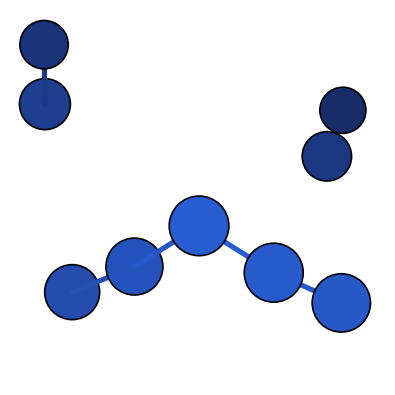
\includegraphics[width=0.8\linewidth]{figs/nonconverged/N9_cation_cation_002_last.png}\\[2pt]
{\small dernier cycle DFT (50 cycles)}
\end{minipage}
\end{figure}
\centerline{\small \texttt{N9\_cation\_cation\_002} -- en cours de fragmentation, 2$+$2$+$5}
\vspace{8pt}
\begin{figure}[H]
\centering
\begin{minipage}{0.46\textwidth}
\centering
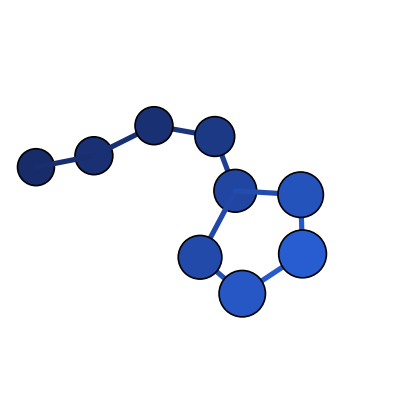
\includegraphics[width=0.8\linewidth]{figs/nonconverged/N9_cation_cation_003_initial.png}\\[2pt]
{\small initiale (xTB, N$_9^{+}$)}
\end{minipage}\hfill
\begin{minipage}{0.46\textwidth}
\centering
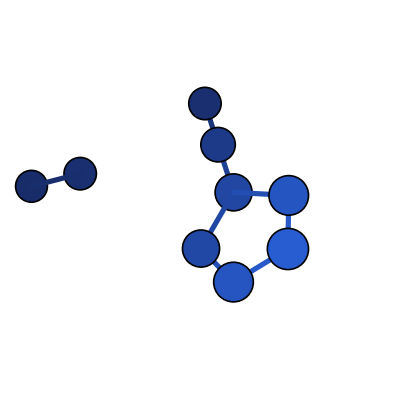
\includegraphics[width=0.8\linewidth]{figs/nonconverged/N9_cation_cation_003_last.png}\\[2pt]
{\small dernier cycle DFT (50 cycles)}
\end{minipage}
\end{figure}
\centerline{\small \texttt{N9\_cation\_cation\_003} -- en cours de fragmentation, 2$+$7}
\vspace{8pt}
\begin{figure}[H]
\centering
\begin{minipage}{0.46\textwidth}
\centering
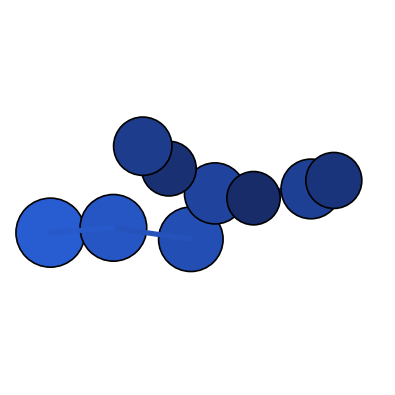
\includegraphics[width=0.8\linewidth]{figs/nonconverged/N9_cation_cation_004_initial.png}\\[2pt]
{\small initiale (xTB, N$_9^{+}$)}
\end{minipage}\hfill
\begin{minipage}{0.46\textwidth}
\centering
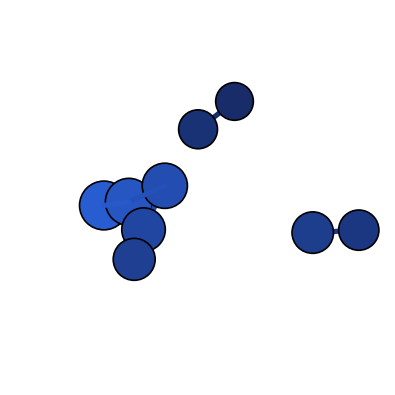
\includegraphics[width=0.8\linewidth]{figs/nonconverged/N9_cation_cation_004_last.png}\\[2pt]
{\small dernier cycle DFT (50 cycles)}
\end{minipage}
\end{figure}
\centerline{\small \texttt{N9\_cation\_cation\_004} -- en cours de fragmentation, 2$+$2$+$5}
\vspace{8pt}
\begin{figure}[H]
\centering
\begin{minipage}{0.46\textwidth}
\centering
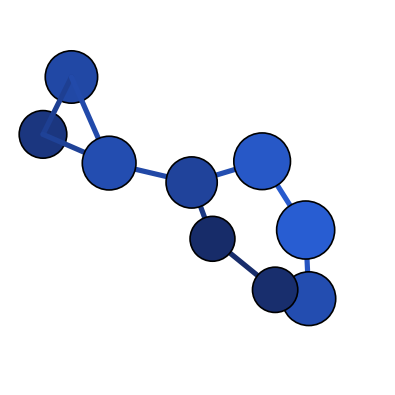
\includegraphics[width=0.8\linewidth]{figs/nonconverged/N9_cation_cation_005_initial.png}\\[2pt]
{\small initiale (xTB, N$_9^{+}$)}
\end{minipage}\hfill
\begin{minipage}{0.46\textwidth}
\centering
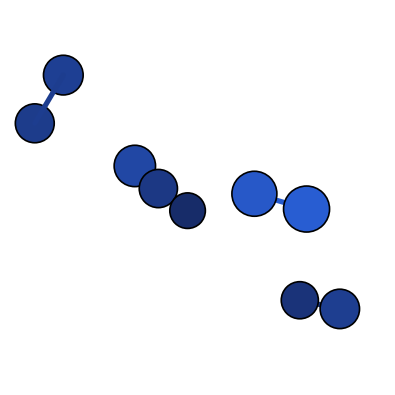
\includegraphics[width=0.8\linewidth]{figs/nonconverged/N9_cation_cation_005_last.png}\\[2pt]
{\small dernier cycle DFT (50 cycles)}
\end{minipage}
\end{figure}
\centerline{\small \texttt{N9\_cation\_cation\_005} -- en cours de fragmentation, 2$+$2$+$2$+$3}
\vspace{8pt}
\begin{figure}[H]
\centering
\begin{minipage}{0.46\textwidth}
\centering
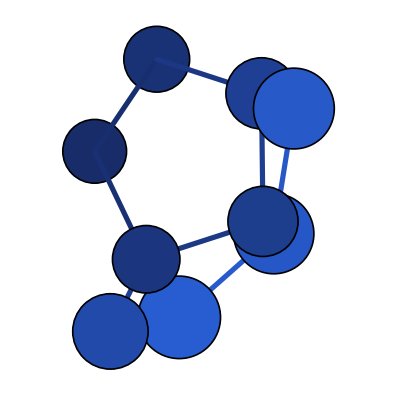
\includegraphics[width=0.8\linewidth]{figs/nonconverged/N9_cation_cation_007_initial.png}\\[2pt]
{\small initiale (xTB, N$_9^{+}$)}
\end{minipage}\hfill
\begin{minipage}{0.46\textwidth}
\centering
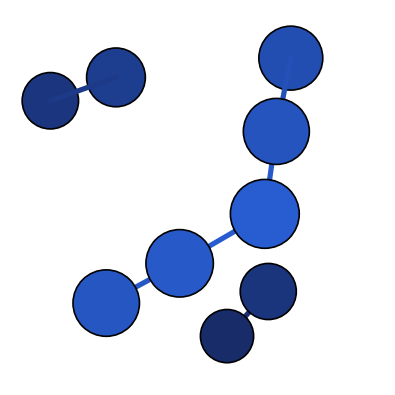
\includegraphics[width=0.8\linewidth]{figs/nonconverged/N9_cation_cation_007_last.png}\\[2pt]
{\small dernier cycle DFT (50 cycles)}
\end{minipage}
\end{figure}
\centerline{\small \texttt{N9\_cation\_cation\_007} -- en cours de fragmentation, 2$+$2$+$5}
\vspace{8pt}
\begin{figure}[H]
\centering
\begin{minipage}{0.46\textwidth}
\centering
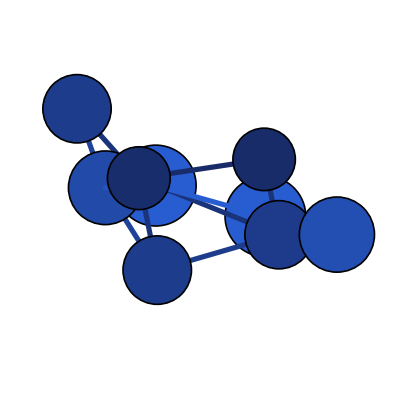
\includegraphics[width=0.8\linewidth]{figs/nonconverged/N9_cation_cation_010_initial.png}\\[2pt]
{\small initiale (xTB, N$_9^{+}$)}
\end{minipage}\hfill
\begin{minipage}{0.46\textwidth}
\centering
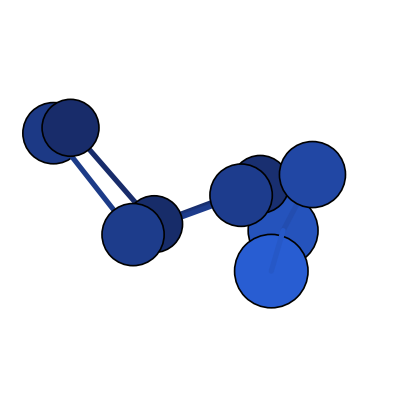
\includegraphics[width=0.8\linewidth]{figs/nonconverged/N9_cation_cation_010_last.png}\\[2pt]
{\small dernier cycle DFT (50 cycles)}
\end{minipage}
\end{figure}
\centerline{\small \texttt{N9\_cation\_cation\_010} -- cluster unique -- non-convergence num\'erique}
\vspace{8pt}
\begin{figure}[H]
\centering
\begin{minipage}{0.46\textwidth}
\centering
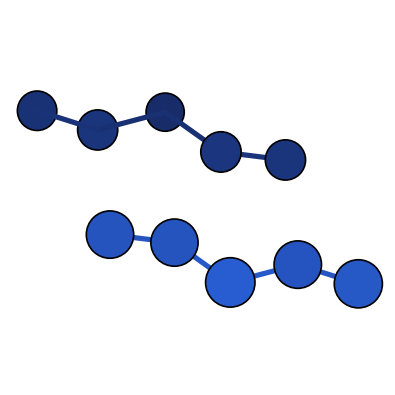
\includegraphics[width=0.8\linewidth]{figs/nonconverged/N10_neutral_neutral_008_initial.png}\\[2pt]
{\small initiale (xTB, N$_10^{0}$)}
\end{minipage}\hfill
\begin{minipage}{0.46\textwidth}
\centering
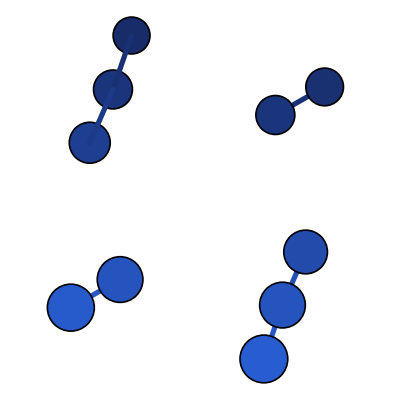
\includegraphics[width=0.8\linewidth]{figs/nonconverged/N10_neutral_neutral_008_last.png}\\[2pt]
{\small dernier cycle DFT (50 cycles)}
\end{minipage}
\end{figure}
\centerline{\small \texttt{N10\_neutral\_neutral\_008} -- en cours de fragmentation, 2$+$2$+$3$+$3}
\vspace{8pt}
\begin{figure}[H]
\centering
\begin{minipage}{0.46\textwidth}
\centering
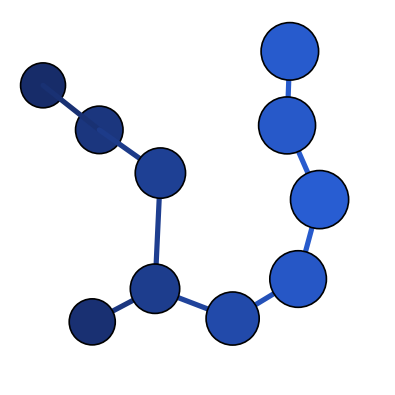
\includegraphics[width=0.8\linewidth]{figs/nonconverged/N10_neutral_neutral_009_initial.png}\\[2pt]
{\small initiale (xTB, N$_10^{0}$)}
\end{minipage}\hfill
\begin{minipage}{0.46\textwidth}
\centering
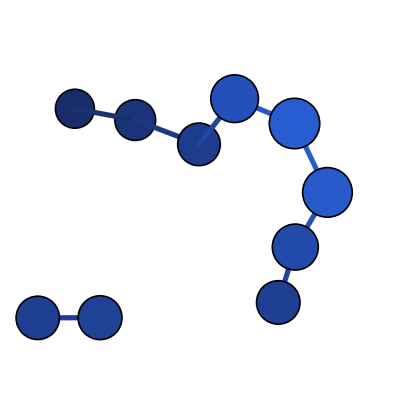
\includegraphics[width=0.8\linewidth]{figs/nonconverged/N10_neutral_neutral_009_last.png}\\[2pt]
{\small dernier cycle DFT (50 cycles)}
\end{minipage}
\end{figure}
\centerline{\small \texttt{N10\_neutral\_neutral\_009} -- en cours de fragmentation, 2$+$8}
\vspace{8pt}
\begin{figure}[H]
\centering
\begin{minipage}{0.46\textwidth}
\centering
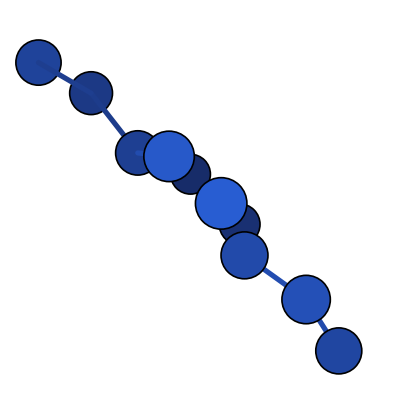
\includegraphics[width=0.8\linewidth]{figs/nonconverged/N10_neutral_neutral_012_initial.png}\\[2pt]
{\small initiale (xTB, N$_10^{0}$)}
\end{minipage}\hfill
\begin{minipage}{0.46\textwidth}
\centering
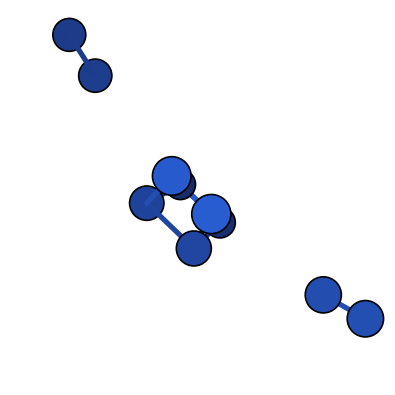
\includegraphics[width=0.8\linewidth]{figs/nonconverged/N10_neutral_neutral_012_last.png}\\[2pt]
{\small dernier cycle DFT (50 cycles)}
\end{minipage}
\end{figure}
\centerline{\small \texttt{N10\_neutral\_neutral\_012} -- en cours de fragmentation, 2$+$2$+$6}
\vspace{8pt}
\begin{figure}[H]
\centering
\begin{minipage}{0.46\textwidth}
\centering
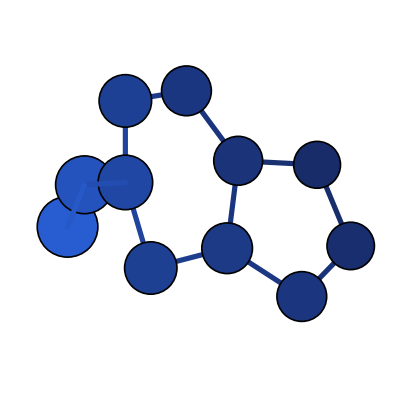
\includegraphics[width=0.8\linewidth]{figs/nonconverged/N11_anion_anion_009_initial.png}\\[2pt]
{\small initiale (xTB, N$_11^{-}$)}
\end{minipage}\hfill
\begin{minipage}{0.46\textwidth}
\centering
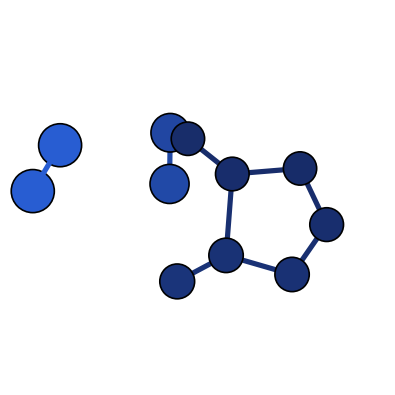
\includegraphics[width=0.8\linewidth]{figs/nonconverged/N11_anion_anion_009_last.png}\\[2pt]
{\small dernier cycle DFT (50 cycles)}
\end{minipage}
\end{figure}
\centerline{\small \texttt{N11\_anion\_anion\_009} -- en cours de fragmentation, 2$+$2$+$7}
\vspace{8pt}
\begin{figure}[H]
\centering
\begin{minipage}{0.46\textwidth}
\centering
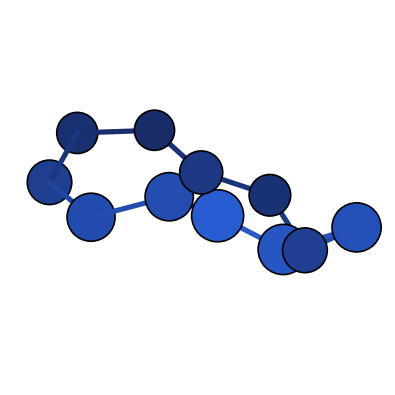
\includegraphics[width=0.8\linewidth]{figs/nonconverged/N11_anion_anion_012_initial.png}\\[2pt]
{\small initiale (xTB, N$_11^{-}$)}
\end{minipage}\hfill
\begin{minipage}{0.46\textwidth}
\centering
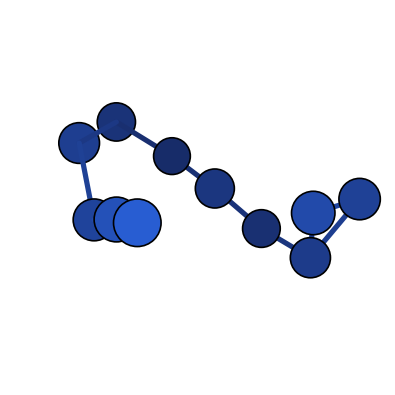
\includegraphics[width=0.8\linewidth]{figs/nonconverged/N11_anion_anion_012_last.png}\\[2pt]
{\small dernier cycle DFT (50 cycles)}
\end{minipage}
\end{figure}
\centerline{\small \texttt{N11\_anion\_anion\_012} -- cluster unique -- non-convergence num\'erique}
\vspace{8pt}
\begin{figure}[H]
\centering
\begin{minipage}{0.46\textwidth}
\centering
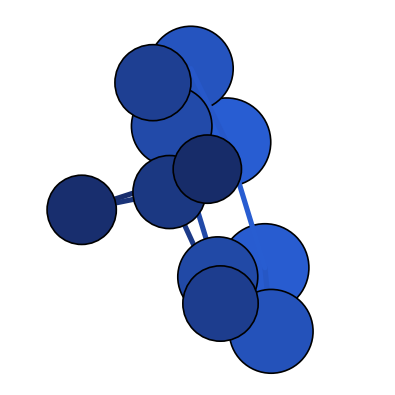
\includegraphics[width=0.8\linewidth]{figs/nonconverged/N11_anion_anion_014_initial.png}\\[2pt]
{\small initiale (xTB, N$_11^{-}$)}
\end{minipage}\hfill
\begin{minipage}{0.46\textwidth}
\centering
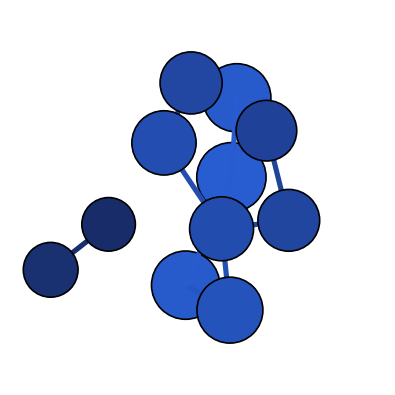
\includegraphics[width=0.8\linewidth]{figs/nonconverged/N11_anion_anion_014_last.png}\\[2pt]
{\small dernier cycle DFT (50 cycles)}
\end{minipage}
\end{figure}
\centerline{\small \texttt{N11\_anion\_anion\_014} -- en cours de fragmentation, 2$+$9}
\vspace{8pt}
\begin{figure}[H]
\centering
\begin{minipage}{0.46\textwidth}
\centering
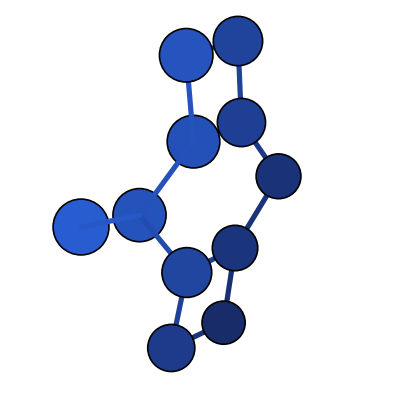
\includegraphics[width=0.8\linewidth]{figs/nonconverged/N11_anion_anion_015_initial.png}\\[2pt]
{\small initiale (xTB, N$_11^{-}$)}
\end{minipage}\hfill
\begin{minipage}{0.46\textwidth}
\centering
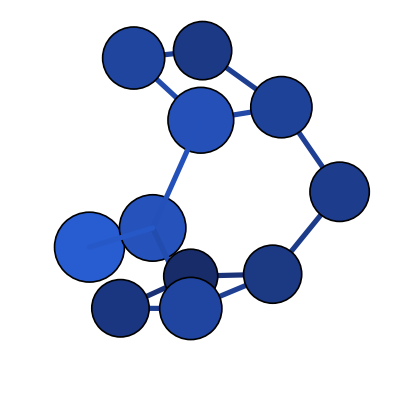
\includegraphics[width=0.8\linewidth]{figs/nonconverged/N11_anion_anion_015_last.png}\\[2pt]
{\small dernier cycle DFT (50 cycles)}
\end{minipage}
\end{figure}
\centerline{\small \texttt{N11\_anion\_anion\_015} -- cluster unique -- non-convergence num\'erique}
\vspace{8pt}
\begin{figure}[H]
\centering
\begin{minipage}{0.46\textwidth}
\centering
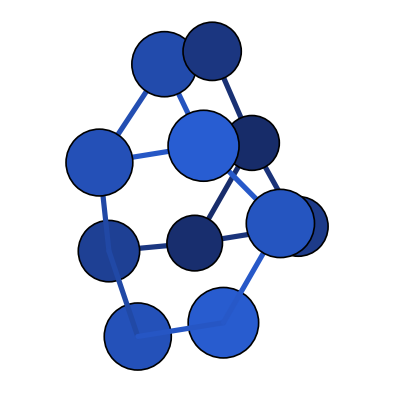
\includegraphics[width=0.8\linewidth]{figs/nonconverged/N11_anion_anion_016_initial.png}\\[2pt]
{\small initiale (xTB, N$_11^{-}$)}
\end{minipage}\hfill
\begin{minipage}{0.46\textwidth}
\centering
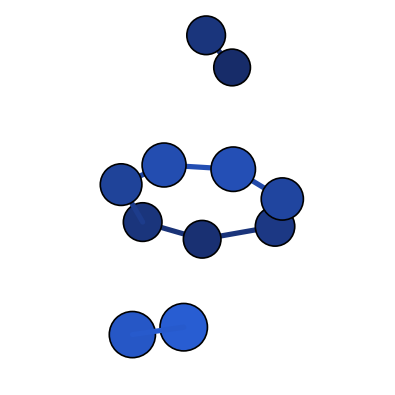
\includegraphics[width=0.8\linewidth]{figs/nonconverged/N11_anion_anion_016_last.png}\\[2pt]
{\small dernier cycle DFT (50 cycles)}
\end{minipage}
\end{figure}
\centerline{\small \texttt{N11\_anion\_anion\_016} -- en cours de fragmentation, 2$+$2$+$7}
\vspace{8pt}
\begin{figure}[H]
\centering
\begin{minipage}{0.46\textwidth}
\centering
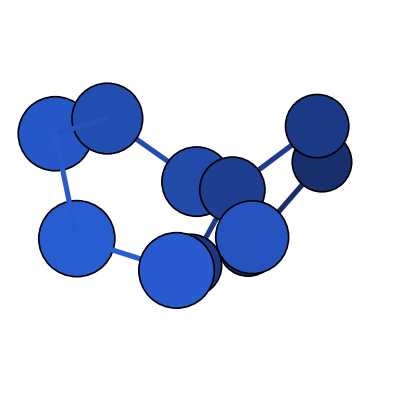
\includegraphics[width=0.8\linewidth]{figs/nonconverged/N11_cation_cation_003_initial.png}\\[2pt]
{\small initiale (xTB, N$_11^{+}$)}
\end{minipage}\hfill
\begin{minipage}{0.46\textwidth}
\centering
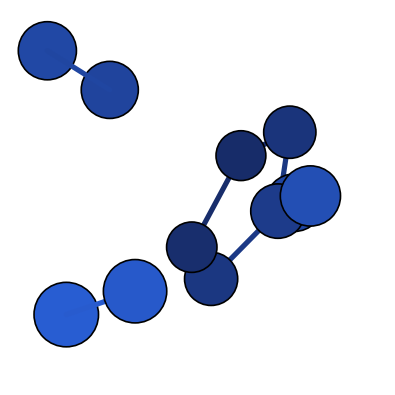
\includegraphics[width=0.8\linewidth]{figs/nonconverged/N11_cation_cation_003_last.png}\\[2pt]
{\small dernier cycle DFT (50 cycles)}
\end{minipage}
\end{figure}
\centerline{\small \texttt{N11\_cation\_cation\_003} -- en cours de fragmentation, 2$+$2$+$7}
\vspace{8pt}
\begin{figure}[H]
\centering
\begin{minipage}{0.46\textwidth}
\centering
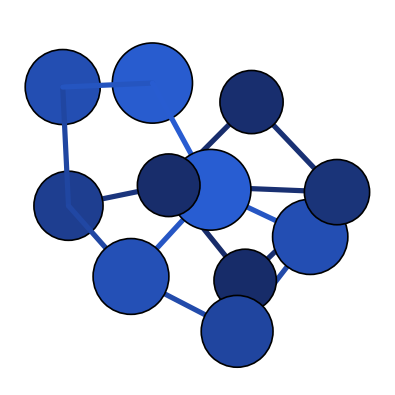
\includegraphics[width=0.8\linewidth]{figs/nonconverged/N11_cation_cation_008_initial.png}\\[2pt]
{\small initiale (xTB, N$_11^{+}$)}
\end{minipage}\hfill
\begin{minipage}{0.46\textwidth}
\centering
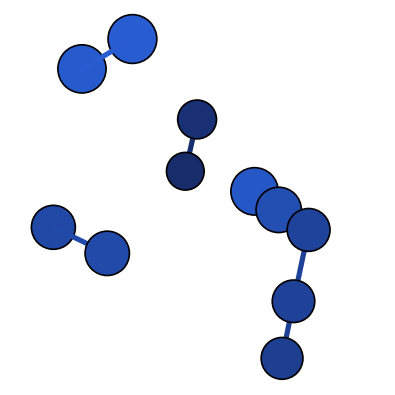
\includegraphics[width=0.8\linewidth]{figs/nonconverged/N11_cation_cation_008_last.png}\\[2pt]
{\small dernier cycle DFT (50 cycles)}
\end{minipage}
\end{figure}
\centerline{\small \texttt{N11\_cation\_cation\_008} -- en cours de fragmentation, 2$+$2$+$2$+$5}
\vspace{8pt}
\begin{figure}[H]
\centering
\begin{minipage}{0.46\textwidth}
\centering
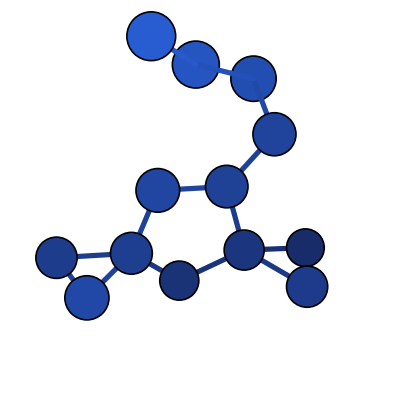
\includegraphics[width=0.8\linewidth]{figs/nonconverged/N13_anion_anion_002_initial.png}\\[2pt]
{\small initiale (xTB, N$_13^{-}$)}
\end{minipage}\hfill
\begin{minipage}{0.46\textwidth}
\centering
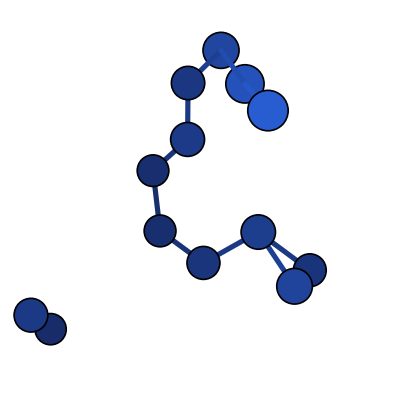
\includegraphics[width=0.8\linewidth]{figs/nonconverged/N13_anion_anion_002_last.png}\\[2pt]
{\small dernier cycle DFT (50 cycles)}
\end{minipage}
\end{figure}
\centerline{\small \texttt{N13\_anion\_anion\_002} -- en cours de fragmentation, 2$+$11}
\vspace{8pt}
\begin{figure}[H]
\centering
\begin{minipage}{0.46\textwidth}
\centering
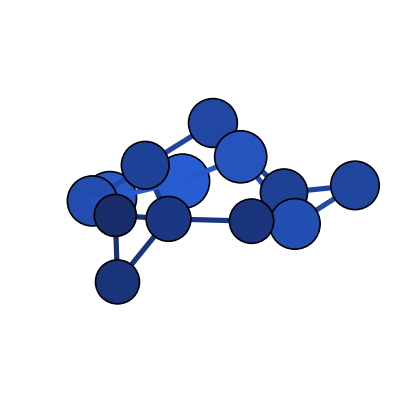
\includegraphics[width=0.8\linewidth]{figs/nonconverged/N13_anion_anion_003_initial.png}\\[2pt]
{\small initiale (xTB, N$_13^{-}$)}
\end{minipage}\hfill
\begin{minipage}{0.46\textwidth}
\centering
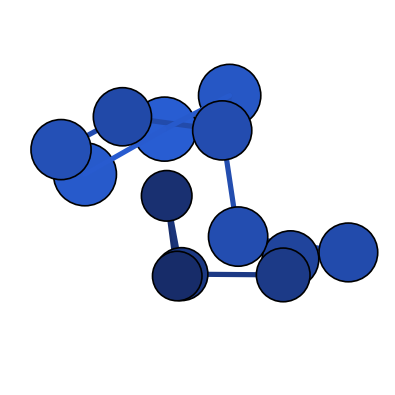
\includegraphics[width=0.8\linewidth]{figs/nonconverged/N13_anion_anion_003_last.png}\\[2pt]
{\small dernier cycle DFT (50 cycles)}
\end{minipage}
\end{figure}
\centerline{\small \texttt{N13\_anion\_anion\_003} -- cluster unique -- non-convergence num\'erique}
\vspace{8pt}
\begin{figure}[H]
\centering
\begin{minipage}{0.46\textwidth}
\centering
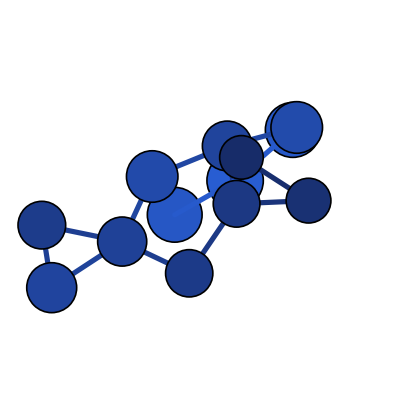
\includegraphics[width=0.8\linewidth]{figs/nonconverged/N13_anion_anion_004_initial.png}\\[2pt]
{\small initiale (xTB, N$_13^{-}$)}
\end{minipage}\hfill
\begin{minipage}{0.46\textwidth}
\centering
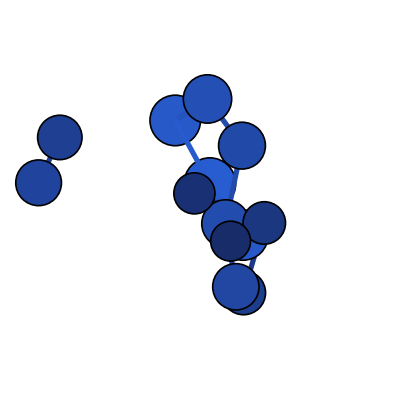
\includegraphics[width=0.8\linewidth]{figs/nonconverged/N13_anion_anion_004_last.png}\\[2pt]
{\small dernier cycle DFT (50 cycles)}
\end{minipage}
\end{figure}
\centerline{\small \texttt{N13\_anion\_anion\_004} -- en cours de fragmentation, 2$+$11}
\vspace{8pt}
\begin{figure}[H]
\centering
\begin{minipage}{0.46\textwidth}
\centering
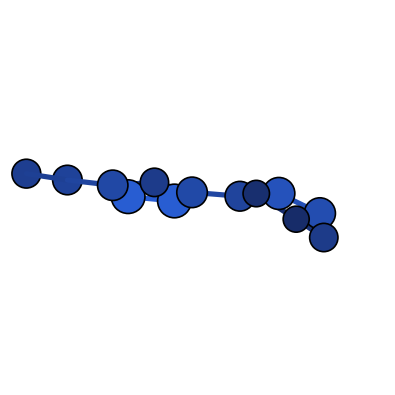
\includegraphics[width=0.8\linewidth]{figs/nonconverged/N13_cation_cation_002_initial.png}\\[2pt]
{\small initiale (xTB, N$_13^{+}$)}
\end{minipage}\hfill
\begin{minipage}{0.46\textwidth}
\centering
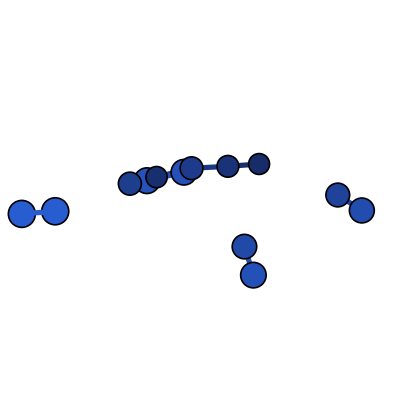
\includegraphics[width=0.8\linewidth]{figs/nonconverged/N13_cation_cation_002_last.png}\\[2pt]
{\small dernier cycle DFT (50 cycles)}
\end{minipage}
\end{figure}
\centerline{\small \texttt{N13\_cation\_cation\_002} -- en cours de fragmentation, 2$+$2$+$2$+$7}
\vspace{8pt}
\begin{figure}[H]
\centering
\begin{minipage}{0.46\textwidth}
\centering
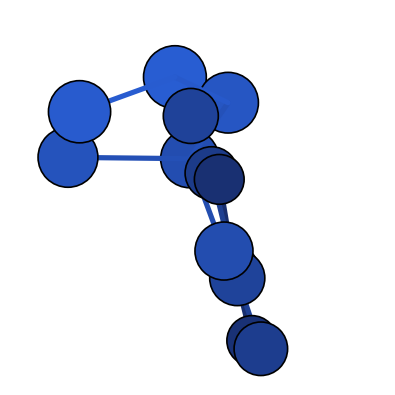
\includegraphics[width=0.8\linewidth]{figs/nonconverged/N13_cation_cation_003_initial.png}\\[2pt]
{\small initiale (xTB, N$_13^{+}$)}
\end{minipage}\hfill
\begin{minipage}{0.46\textwidth}
\centering
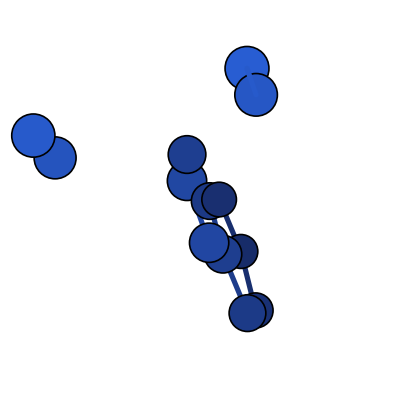
\includegraphics[width=0.8\linewidth]{figs/nonconverged/N13_cation_cation_003_last.png}\\[2pt]
{\small dernier cycle DFT (50 cycles)}
\end{minipage}
\end{figure}
\centerline{\small \texttt{N13\_cation\_cation\_003} -- en cours de fragmentation, 2$+$2$+$9}
\vspace{8pt}
\bigskip\noindent\textit{L\'egende g\'en\'erale, Figure~S2~:} sph\`eres bleues reli\'ees par des b\^atonnets = atomes N et liaisons N--N (mod\`ele boules-b\^atonnets, rendu depuis les coordonn\'ees cart\'esiennes .xyz) ; paires group\'ees par candidat, g\'eom\'etrie initiale GFN2-xTB \`a gauche et derni\`ere g\'eom\'etrie de la trajectoire d'optimisation DFT (non converg\'ee) \`a droite, pour les 35 candidats non converg\'es (Tableau~S2).

\subsection{Structures avec fr\'equence imaginaire}
\label{sec:si-imaginary}

\noindent\textbf{Table S2.} Structures avec au moins une fr\'equence imaginaire (pas encore de vrai minimum). ``Max.\ imaginaire''~: la fr\'equence de plus grande amplitude parmi les modes imaginaires (mode dominant de la coordonn\'ee de r\'eaction vers le vrai minimum). $\Delta H$~: \'energie relative au ground-state DFT de la m\^eme composition (kcal/mol, niveau DFT si disponible sinon xTB) -- \`a rapprocher de la fr\'equence pour rep\'erer une \'eventuelle corr\'elation entre instabilit\'e vibrationnelle et haute \'energie relative. \'A reprendre manuellement (distorsion le long de ce mode puis r\'eoptimisation) avant validation finale.\par\vspace{4pt}
\begin{longtable}{@{}p{4.0cm}ccrrp{1.7cm}c@{}}
\scriptsize
\label{tab:imaginary}\\
\toprule
\textbf{Nom} & \textbf{N} & \textbf{n modes} & \textbf{Max.\ imag.\ (cm$^{-1}$)} & \textbf{Intensit\'e (km/mol)} & \textbf{$\Delta H$ (kcal/mol)} & \textbf{Frag.} \\
\midrule\endfirsthead
\multicolumn{7}{c}{\small (suite)}\\ \toprule\endhead
\bottomrule\endfoot
\bottomrule\endlastfoot
\texttt{N4\_neutral\_neutral\_002} & 4 & 1 & -249.3 & -- & 16.85 (DFT) &  \\
\texttt{N4\_neutral\_neutral\_003} & 4 & 1 & -567.2 & -- & 33.07 (DFT) &  \\
\texttt{N5\_anion\_anion\_006} & 5 & 1 & -211.7 & -- & 104.46 (DFT) &  \\
\texttt{N5\_anion\_anion\_009} & 5 & 1 & -15.9 & -- & 66.07 (DFT) & \checkmark \\
\texttt{N5\_cation\_cation\_007} & 5 & 2 & -92.3 & -- & 34.45 (DFT) & \checkmark \\
\texttt{N6\_neutral\_neutral\_004} & 6 & 3 & -26.9 & -- & -172.76 (DFT) & \checkmark \\
\texttt{N6\_neutral\_neutral\_010} & 6 & 2 & -779.2 & -- & 149.79 (DFT) &  \\
\texttt{N7\_anion\_anion\_003} & 7 & 1 & -210.7 & -- & 20.91 (DFT) &  \\
\texttt{N7\_anion\_anion\_007} & 7 & 1 & -746.3 & -- & 35.75 (DFT) &  \\
\texttt{N7\_anion\_anion\_009} & 7 & 1 & -112.9 & -- & 54.95 (DFT) &  \\
\texttt{N7\_anion\_anion\_013} & 7 & 1 & -238.3 & -- & 9.42 (DFT) &  \\
\texttt{N7\_anion\_anion\_016} & 7 & 1 & -275.3 & -- & 40.69 (DFT) &  \\
\texttt{N7\_anion\_anion\_017} & 7 & 1 & -209.3 & -- & 80.80 (DFT) &  \\
\texttt{N7\_anion\_anion\_018} & 7 & 1 & -24.6 & -- & 79.33 (DFT) &  \\
\texttt{N7\_anion\_anion\_020} & 7 & 2 & -1284.2 & -- & 179.57 (DFT) &  \\
\texttt{N7\_cation\_cation\_005} & 7 & 2 & -697.7 & -- & 189.69 (DFT) &  \\
\texttt{N7\_cation\_cation\_006} & 7 & 1 & -297.4 & -- & 200.56 (DFT) &  \\
\texttt{N9\_anion\_anion\_006} & 9 & 2 & -285.6 & -- & 27.56 (DFT) &  \\
\texttt{N10\_neutral\_neutral\_013} & 10 & 2 & -255.6 & -- & 193.75 (DFT) &  \\
\texttt{N11\_anion\_anion\_001} & 11 & 2 & -66.8 & -- & 0.00 (DFT) &  \\
\texttt{N11\_anion\_anion\_002} & 11 & 1 & -44.4 & -- & 38.48 (DFT) &  \\
\texttt{N11\_anion\_anion\_003} & 11 & 2 & -322.0 & -- & 109.19 (DFT) &  \\
\texttt{N11\_anion\_anion\_004} & 11 & 1 & -79.0 & -- & 92.16 (DFT) &  \\
\texttt{N11\_anion\_anion\_005} & 11 & 1 & -63.6 & -- & 74.39 (DFT) &  \\
\texttt{N11\_anion\_anion\_010} & 11 & 1 & -42.9 & -- & 102.27 (DFT) &  \\
\texttt{N11\_cation\_cation\_002} & 11 & 1 & -138.2 & -- & 0.00 (DFT) &  \\
\texttt{N11\_cation\_cation\_005} & 11 & 1 & -248.0 & -- & 45.85 (DFT) &  \\
\texttt{N12\_neutral\_neutral\_005} & 12 & 1 & -28.0 & -- & 138.12 (DFT) &  \\
\texttt{N14\_neutral\_neutral\_001} & 14 & 1 & -81.0 & -- & 0.00 (DFT) &  \\
\texttt{N14\_neutral\_neutral\_004} & 14 & 6 & -36.3 & -- & -250.59 (DFT) & \checkmark \\
\end{longtable}

\subsection{Structures optimis\'ees confirm\'ees}
\label{sec:si-confirmed}

Les 110 candidats confirm\'es comme vrais minima \textbf{non-fragment\'es}
au moment de la r\'edaction, deux par ligne. Trois figures, class\'ees
par nombre d'atomes croissant puis par stabilit\'e au sein de chaque
formule~: Figure~S3 (neutres), Figure~S4 (cations), Figure~S5 (anions).
Chaque structure porte son nom, son groupe ponctuel, son $\Delta H$
(kcal/mol), le niveau de th\'eorie de ce $\Delta H$ (DFT ou xTB si le DFT
n'est pas encore termin\'e), et sa r\'ef\'erence (num\'ero(s) d'article ou
\emph{our work}). Comme dans les Tableaux~2--4~: $\Delta H$ = \'energie
d'isom\'erisation \`a N et charge fix\'es, N$_x^{q}$(isom\`ere $i$)
$\rightarrow$ N$_x^{q}$(isom\`ere le plus stable non-fragment\'e de la
m\^eme formule), $\Delta H = E(i) - E_{\mathrm{stable}}$ (isom\`ere le
plus stable $=0$).

\begin{figure}[H]
\centering
\begin{minipage}{0.46\textwidth}
\centering
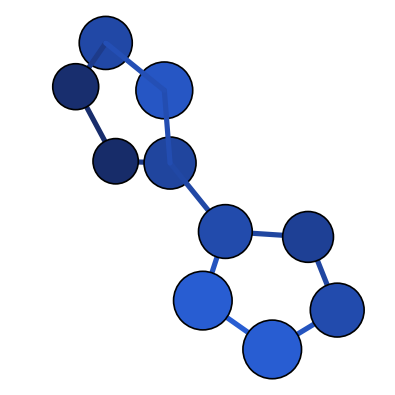
\includegraphics[width=0.85\linewidth]{figs/N10_neutral_neutral_001.png}\\[2pt]
{\small \texttt{N10\_neutral\_neutral\_001} -- C2}
\end{minipage}\hfill
\begin{minipage}{0.46\textwidth}
\centering
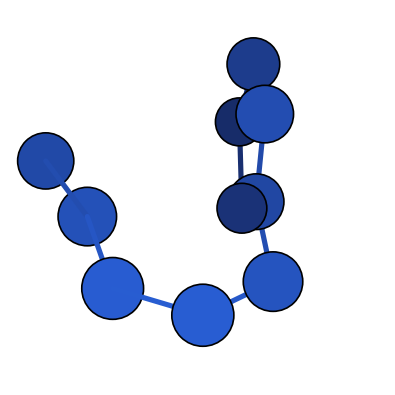
\includegraphics[width=0.85\linewidth]{figs/N10_neutral_neutral_002.png}\\[2pt]
{\small \texttt{N10\_neutral\_neutral\_002} -- C1}
\end{minipage}\hfill
\end{figure}
\begin{figure}[H]
\centering
\begin{minipage}{0.46\textwidth}
\centering
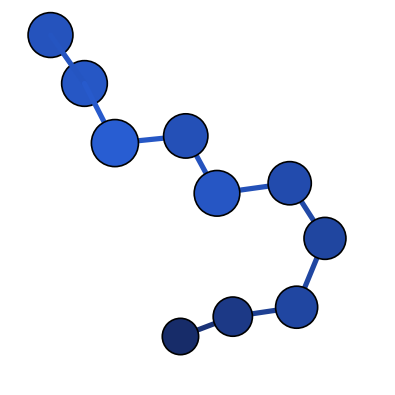
\includegraphics[width=0.85\linewidth]{figs/N10_neutral_neutral_003.png}\\[2pt]
{\small \texttt{N10\_neutral\_neutral\_003} -- C1}
\end{minipage}\hfill
\begin{minipage}{0.46\textwidth}
\centering
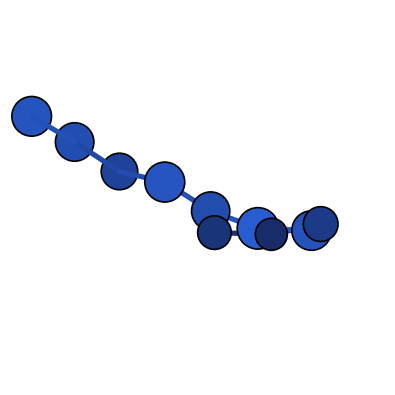
\includegraphics[width=0.85\linewidth]{figs/N10_neutral_neutral_004.png}\\[2pt]
{\small \texttt{N10\_neutral\_neutral\_004} -- C1}
\end{minipage}\hfill
\end{figure}
\begin{figure}[H]
\centering
\begin{minipage}{0.46\textwidth}
\centering
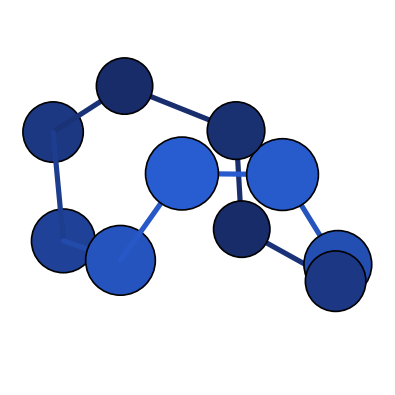
\includegraphics[width=0.85\linewidth]{figs/N10_neutral_neutral_005.png}\\[2pt]
{\small \texttt{N10\_neutral\_neutral\_005} -- C1}
\end{minipage}\hfill
\begin{minipage}{0.46\textwidth}
\centering
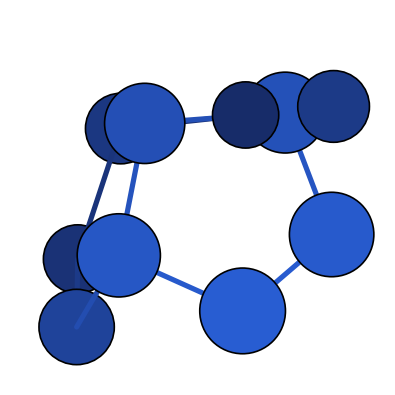
\includegraphics[width=0.85\linewidth]{figs/N10_neutral_neutral_006.png}\\[2pt]
{\small \texttt{N10\_neutral\_neutral\_006} -- Cs}
\end{minipage}\hfill
\end{figure}
\begin{figure}[H]
\centering
\begin{minipage}{0.46\textwidth}
\centering
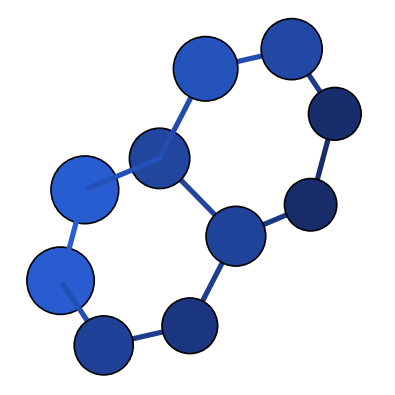
\includegraphics[width=0.85\linewidth]{figs/N10_neutral_neutral_007.png}\\[2pt]
{\small \texttt{N10\_neutral\_neutral\_007} -- Cs}
\end{minipage}\hfill
\begin{minipage}{0.46\textwidth}
\centering
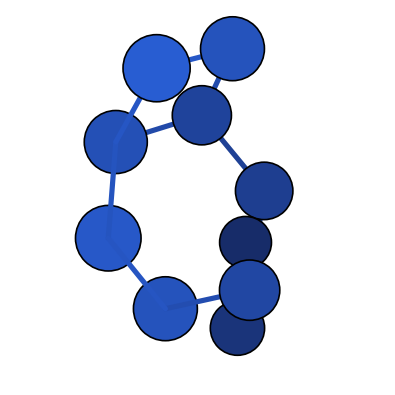
\includegraphics[width=0.85\linewidth]{figs/N10_neutral_neutral_010.png}\\[2pt]
{\small \texttt{N10\_neutral\_neutral\_010} -- C1}
\end{minipage}\hfill
\end{figure}
\begin{figure}[H]
\centering
\begin{minipage}{0.46\textwidth}
\centering
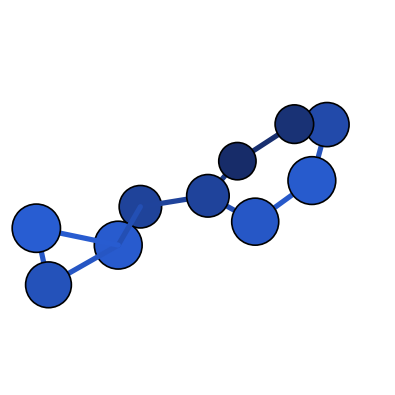
\includegraphics[width=0.85\linewidth]{figs/N10_neutral_neutral_011.png}\\[2pt]
{\small \texttt{N10\_neutral\_neutral\_011} -- C1}
\end{minipage}\hfill
\begin{minipage}{0.46\textwidth}
\centering
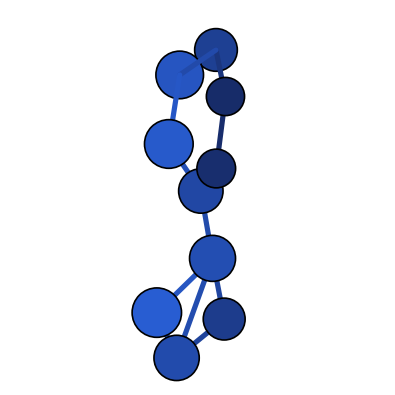
\includegraphics[width=0.85\linewidth]{figs/N10_neutral_neutral_014.png}\\[2pt]
{\small \texttt{N10\_neutral\_neutral\_014} -- C1}
\end{minipage}\hfill
\end{figure}
\begin{figure}[H]
\centering
\begin{minipage}{0.46\textwidth}
\centering
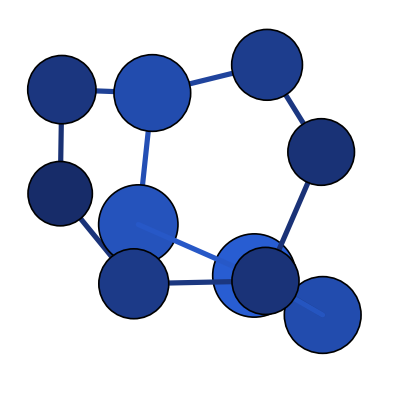
\includegraphics[width=0.85\linewidth]{figs/N10_neutral_neutral_015.png}\\[2pt]
{\small \texttt{N10\_neutral\_neutral\_015} -- C2}
\end{minipage}\hfill
\begin{minipage}{0.46\textwidth}
\centering
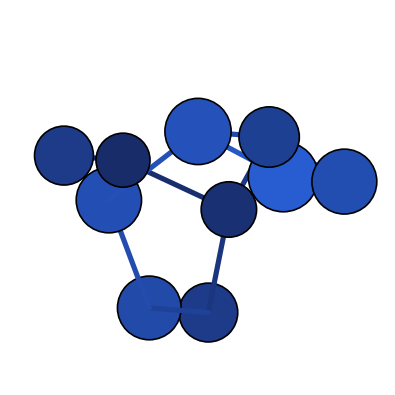
\includegraphics[width=0.85\linewidth]{figs/N10_neutral_neutral_016.png}\\[2pt]
{\small \texttt{N10\_neutral\_neutral\_016} -- C1}
\end{minipage}\hfill
\end{figure}
\begin{figure}[H]
\centering
\begin{minipage}{0.46\textwidth}
\centering
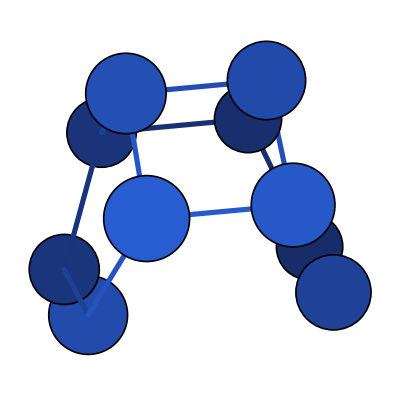
\includegraphics[width=0.85\linewidth]{figs/N10_neutral_neutral_017.png}\\[2pt]
{\small \texttt{N10\_neutral\_neutral\_017} -- C2v}
\end{minipage}\hfill
\begin{minipage}{0.46\textwidth}
\centering
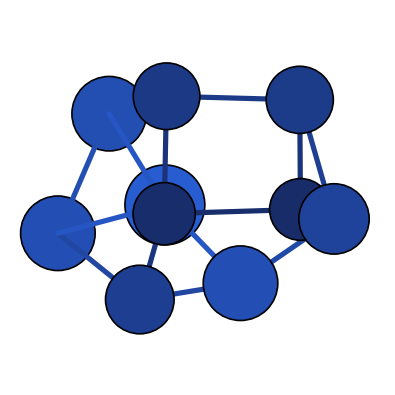
\includegraphics[width=0.85\linewidth]{figs/N10_neutral_neutral_018.png}\\[2pt]
{\small \texttt{N10\_neutral\_neutral\_018} -- C2}
\end{minipage}\hfill
\end{figure}
\begin{figure}[H]
\centering
\begin{minipage}{0.46\textwidth}
\centering
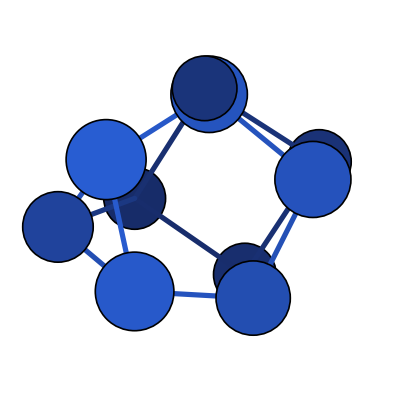
\includegraphics[width=0.85\linewidth]{figs/N10_neutral_neutral_019.png}\\[2pt]
{\small \texttt{N10\_neutral\_neutral\_019} -- C3v}
\end{minipage}\hfill
\begin{minipage}{0.46\textwidth}
\centering
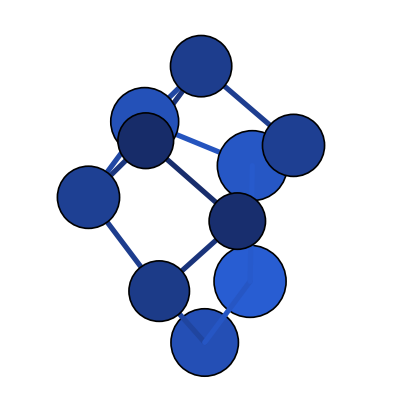
\includegraphics[width=0.85\linewidth]{figs/N10_neutral_neutral_020.png}\\[2pt]
{\small \texttt{N10\_neutral\_neutral\_020} -- C2}
\end{minipage}\hfill
\end{figure}
\begin{figure}[H]
\centering
\begin{minipage}{0.46\textwidth}
\centering
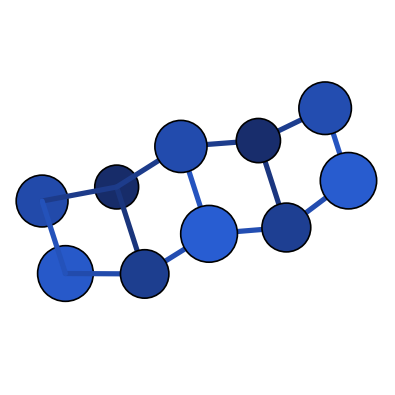
\includegraphics[width=0.85\linewidth]{figs/N10_neutral_neutral_021.png}\\[2pt]
{\small \texttt{N10\_neutral\_neutral\_021} -- C2v}
\end{minipage}\hfill
\begin{minipage}{0.46\textwidth}
\centering
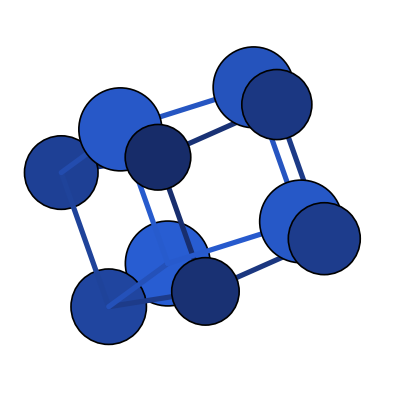
\includegraphics[width=0.85\linewidth]{figs/N10_neutral_neutral_022.png}\\[2pt]
{\small \texttt{N10\_neutral\_neutral\_022} -- D5h}
\end{minipage}\hfill
\end{figure}
\begin{figure}[H]
\centering
\begin{minipage}{0.46\textwidth}
\centering
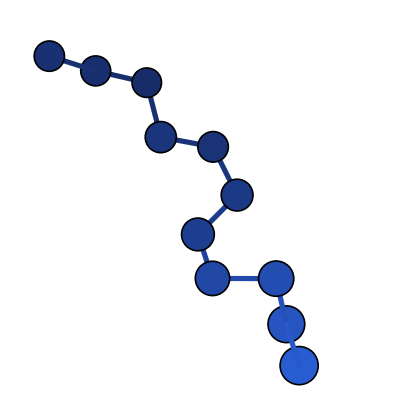
\includegraphics[width=0.85\linewidth]{figs/N11_anion_anion_006.png}\\[2pt]
{\small \texttt{N11\_anion\_anion\_006} -- C1}
\end{minipage}\hfill
\begin{minipage}{0.46\textwidth}
\centering
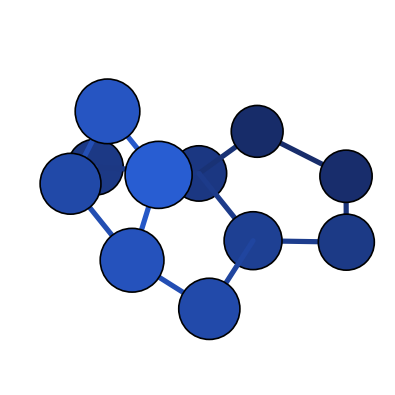
\includegraphics[width=0.85\linewidth]{figs/N11_anion_anion_007.png}\\[2pt]
{\small \texttt{N11\_anion\_anion\_007} -- Cs}
\end{minipage}\hfill
\end{figure}
\begin{figure}[H]
\centering
\begin{minipage}{0.46\textwidth}
\centering
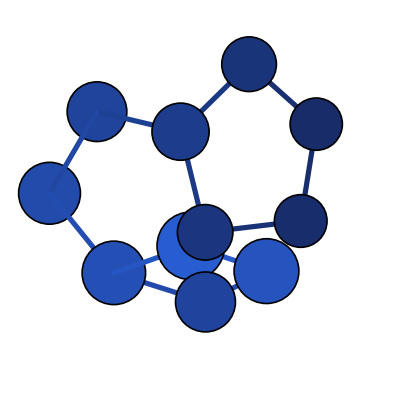
\includegraphics[width=0.85\linewidth]{figs/N11_anion_anion_008.png}\\[2pt]
{\small \texttt{N11\_anion\_anion\_008} -- C1}
\end{minipage}\hfill
\begin{minipage}{0.46\textwidth}
\centering
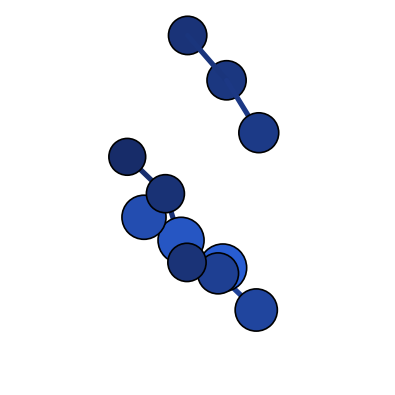
\includegraphics[width=0.85\linewidth]{figs/N11_anion_anion_011.png}\\[2pt]
{\small \texttt{N11\_anion\_anion\_011} -- C1}
\end{minipage}\hfill
\end{figure}
\begin{figure}[H]
\centering
\begin{minipage}{0.46\textwidth}
\centering
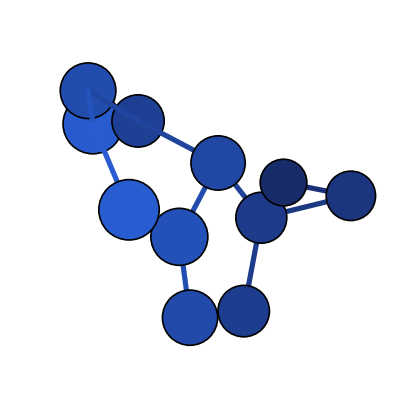
\includegraphics[width=0.85\linewidth]{figs/N11_anion_anion_013.png}\\[2pt]
{\small \texttt{N11\_anion\_anion\_013} -- C1}
\end{minipage}\hfill
\begin{minipage}{0.46\textwidth}
\centering
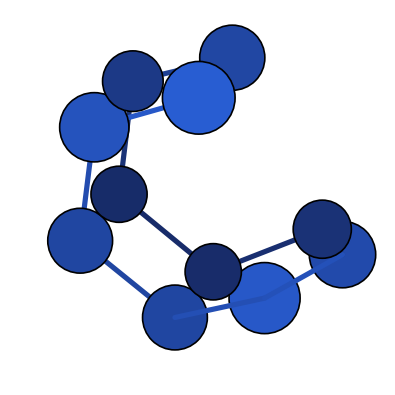
\includegraphics[width=0.85\linewidth]{figs/N11_anion_anion_017.png}\\[2pt]
{\small \texttt{N11\_anion\_anion\_017} -- C1}
\end{minipage}\hfill
\end{figure}
\begin{figure}[H]
\centering
\begin{minipage}{0.46\textwidth}
\centering
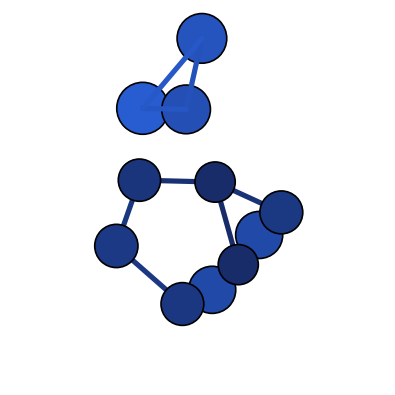
\includegraphics[width=0.85\linewidth]{figs/N11_anion_anion_018.png}\\[2pt]
{\small \texttt{N11\_anion\_anion\_018} -- C1}
\end{minipage}\hfill
\begin{minipage}{0.46\textwidth}
\centering
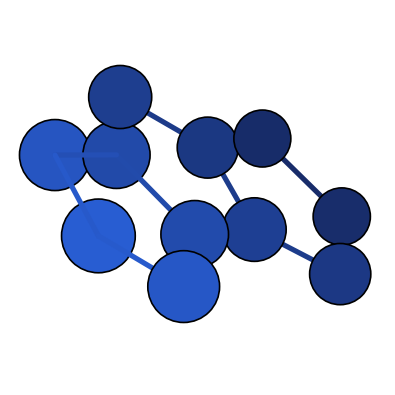
\includegraphics[width=0.85\linewidth]{figs/N11_cation_cation_001.png}\\[2pt]
{\small \texttt{N11\_cation\_cation\_001} -- C2v}
\end{minipage}\hfill
\end{figure}
\begin{figure}[H]
\centering
\begin{minipage}{0.46\textwidth}
\centering
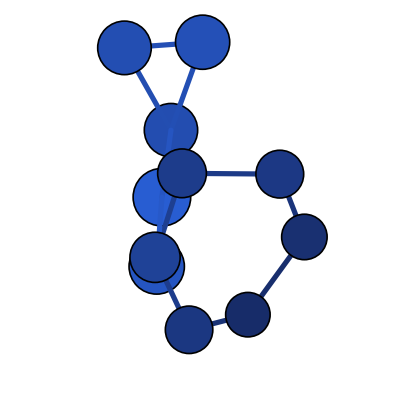
\includegraphics[width=0.85\linewidth]{figs/N11_cation_cation_006.png}\\[2pt]
{\small \texttt{N11\_cation\_cation\_006} -- C1}
\end{minipage}\hfill
\begin{minipage}{0.46\textwidth}
\centering
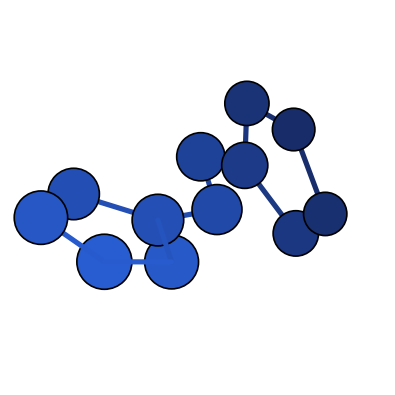
\includegraphics[width=0.85\linewidth]{figs/N12_cation_cation_001.png}\\[2pt]
{\small \texttt{N12\_cation\_cation\_001} -- C1}
\end{minipage}\hfill
\end{figure}
\begin{figure}[H]
\centering
\begin{minipage}{0.46\textwidth}
\centering
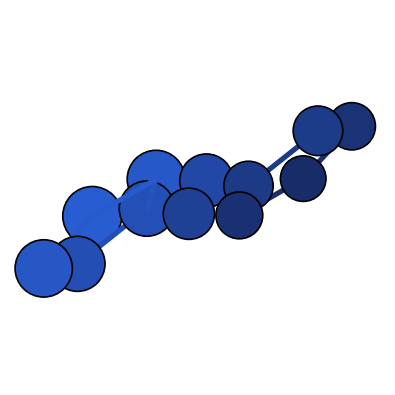
\includegraphics[width=0.85\linewidth]{figs/N12_neutral_neutral_001.png}\\[2pt]
{\small \texttt{N12\_neutral\_neutral\_001} -- C1}
\end{minipage}\hfill
\begin{minipage}{0.46\textwidth}
\centering
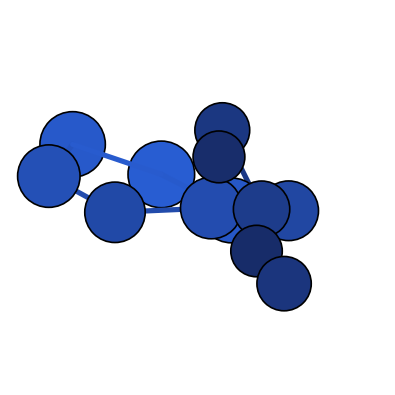
\includegraphics[width=0.85\linewidth]{figs/N12_neutral_neutral_002.png}\\[2pt]
{\small \texttt{N12\_neutral\_neutral\_002} -- C1}
\end{minipage}\hfill
\end{figure}
\begin{figure}[H]
\centering
\begin{minipage}{0.46\textwidth}
\centering
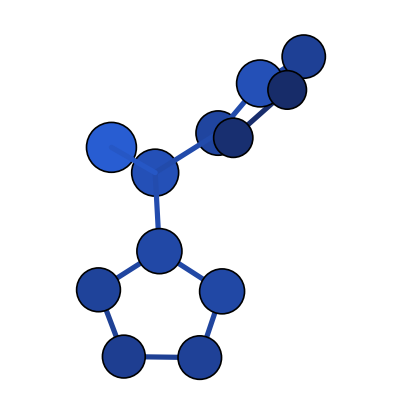
\includegraphics[width=0.85\linewidth]{figs/N12_neutral_neutral_003.png}\\[2pt]
{\small \texttt{N12\_neutral\_neutral\_003} -- C1}
\end{minipage}\hfill
\begin{minipage}{0.46\textwidth}
\centering
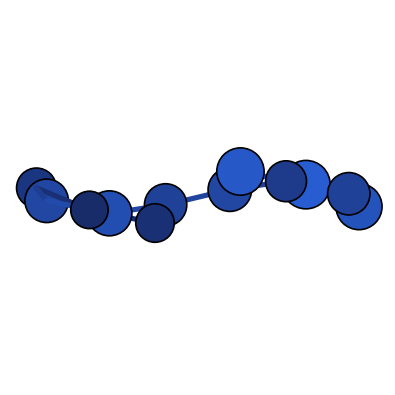
\includegraphics[width=0.85\linewidth]{figs/N12_neutral_neutral_004.png}\\[2pt]
{\small \texttt{N12\_neutral\_neutral\_004} -- Cs}
\end{minipage}\hfill
\end{figure}
\begin{figure}[H]
\centering
\begin{minipage}{0.46\textwidth}
\centering
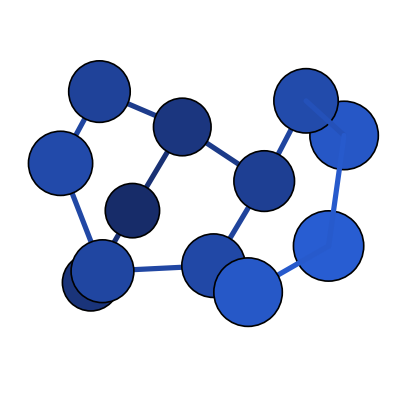
\includegraphics[width=0.85\linewidth]{figs/N12_neutral_neutral_006.png}\\[2pt]
{\small \texttt{N12\_neutral\_neutral\_006} -- C1}
\end{minipage}\hfill
\begin{minipage}{0.46\textwidth}
\centering
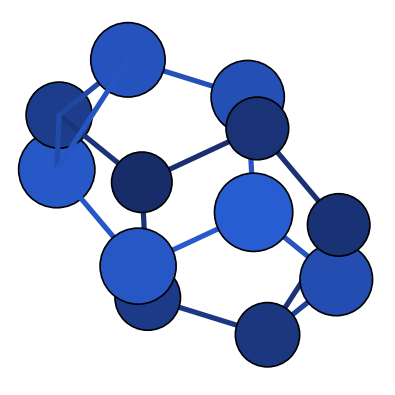
\includegraphics[width=0.85\linewidth]{figs/N12_neutral_neutral_007.png}\\[2pt]
{\small \texttt{N12\_neutral\_neutral\_007} -- D3d}
\end{minipage}\hfill
\end{figure}
\begin{figure}[H]
\centering
\begin{minipage}{0.46\textwidth}
\centering
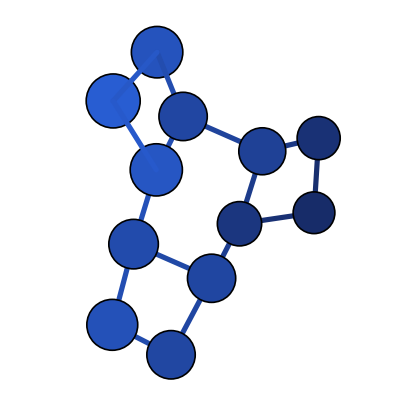
\includegraphics[width=0.85\linewidth]{figs/N12_neutral_neutral_008.png}\\[2pt]
{\small \texttt{N12\_neutral\_neutral\_008} -- C1}
\end{minipage}\hfill
\begin{minipage}{0.46\textwidth}
\centering
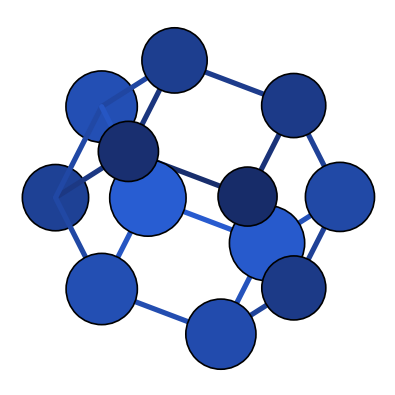
\includegraphics[width=0.85\linewidth]{figs/N12_neutral_neutral_009.png}\\[2pt]
{\small \texttt{N12\_neutral\_neutral\_009} -- D6h}
\end{minipage}\hfill
\end{figure}
\begin{figure}[H]
\centering
\begin{minipage}{0.46\textwidth}
\centering
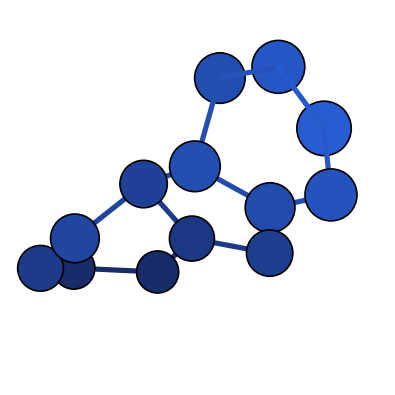
\includegraphics[width=0.85\linewidth]{figs/N13_anion_anion_001.png}\\[2pt]
{\small \texttt{N13\_anion\_anion\_001} -- C1}
\end{minipage}\hfill
\begin{minipage}{0.46\textwidth}
\centering
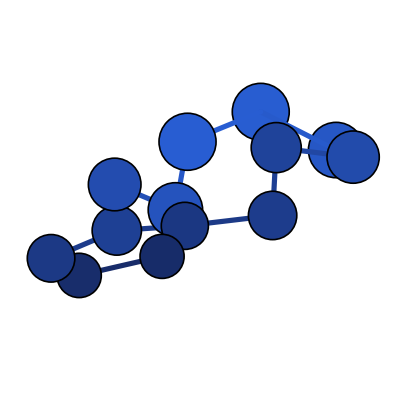
\includegraphics[width=0.85\linewidth]{figs/N13_cation_cation_001.png}\\[2pt]
{\small \texttt{N13\_cation\_cation\_001} -- C1}
\end{minipage}\hfill
\end{figure}
\begin{figure}[H]
\centering
\begin{minipage}{0.46\textwidth}
\centering
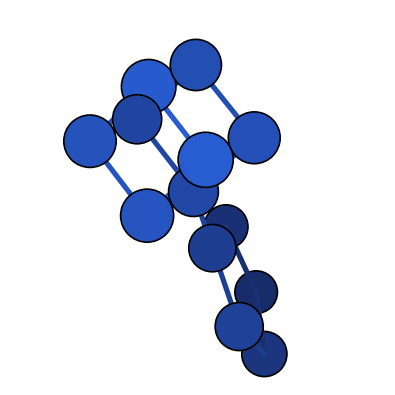
\includegraphics[width=0.85\linewidth]{figs/N13_cation_cation_004.png}\\[2pt]
{\small \texttt{N13\_cation\_cation\_004} -- C1}
\end{minipage}\hfill
\begin{minipage}{0.46\textwidth}
\centering
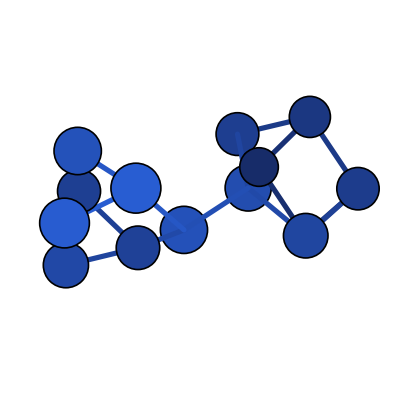
\includegraphics[width=0.85\linewidth]{figs/N14_neutral_neutral_005.png}\\[2pt]
{\small \texttt{N14\_neutral\_neutral\_005} -- C2}
\end{minipage}\hfill
\end{figure}
\begin{figure}[H]
\centering
\begin{minipage}{0.46\textwidth}
\centering
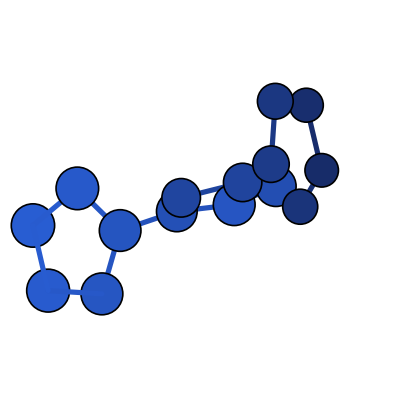
\includegraphics[width=0.85\linewidth]{figs/N15_cation_cation_001.png}\\[2pt]
{\small \texttt{N15\_cation\_cation\_001} -- C1}
\end{minipage}\hfill
\begin{minipage}{0.46\textwidth}
\centering
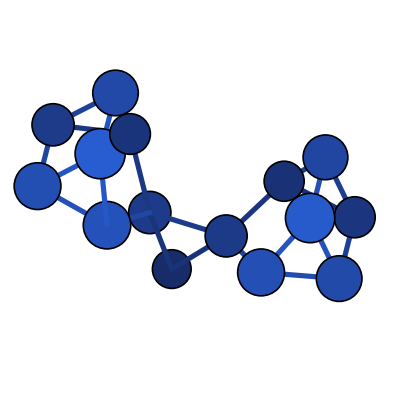
\includegraphics[width=0.85\linewidth]{figs/N15_cation_cation_002.png}\\[2pt]
{\small \texttt{N15\_cation\_cation\_002} -- C1}
\end{minipage}\hfill
\end{figure}
\begin{figure}[H]
\centering
\begin{minipage}{0.46\textwidth}
\centering
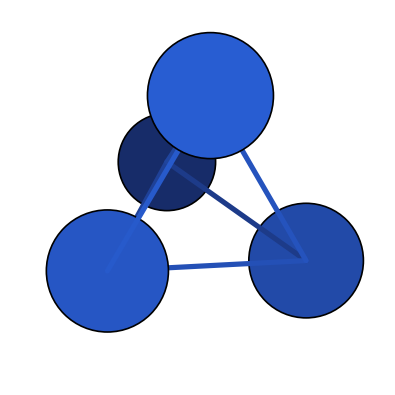
\includegraphics[width=0.85\linewidth]{figs/N4_neutral_neutral_001.png}\\[2pt]
{\small \texttt{N4\_neutral\_neutral\_001} -- Td}
\end{minipage}\hfill
\begin{minipage}{0.46\textwidth}
\centering
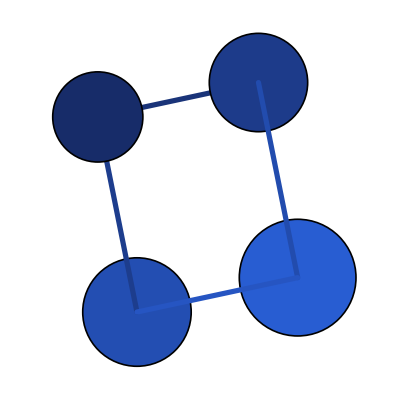
\includegraphics[width=0.85\linewidth]{figs/N4_neutral_neutral_004.png}\\[2pt]
{\small \texttt{N4\_neutral\_neutral\_004} -- D2h}
\end{minipage}\hfill
\end{figure}
\begin{figure}[H]
\centering
\begin{minipage}{0.46\textwidth}
\centering
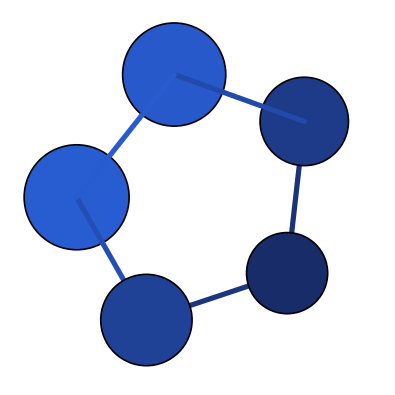
\includegraphics[width=0.85\linewidth]{figs/N5_anion_anion_001.png}\\[2pt]
{\small \texttt{N5\_anion\_anion\_001} -- D5h}
\end{minipage}\hfill
\begin{minipage}{0.46\textwidth}
\centering
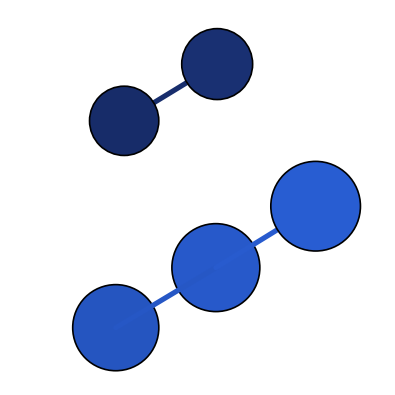
\includegraphics[width=0.85\linewidth]{figs/N5_anion_anion_002.png}\\[2pt]
{\small \texttt{N5\_anion\_anion\_002} -- C1}
\end{minipage}\hfill
\end{figure}
\begin{figure}[H]
\centering
\begin{minipage}{0.46\textwidth}
\centering
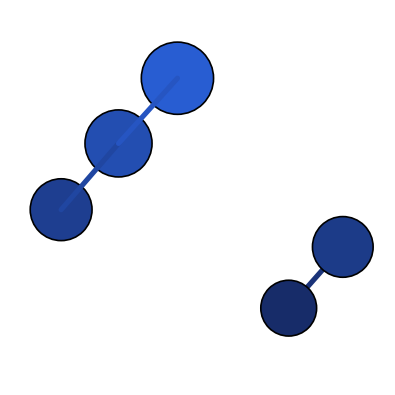
\includegraphics[width=0.85\linewidth]{figs/N5_anion_anion_003.png}\\[2pt]
{\small \texttt{N5\_anion\_anion\_003} -- C1}
\end{minipage}\hfill
\begin{minipage}{0.46\textwidth}
\centering
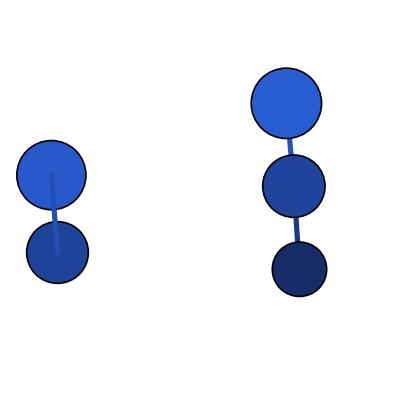
\includegraphics[width=0.85\linewidth]{figs/N5_anion_anion_004.png}\\[2pt]
{\small \texttt{N5\_anion\_anion\_004} -- C1}
\end{minipage}\hfill
\end{figure}
\begin{figure}[H]
\centering
\begin{minipage}{0.46\textwidth}
\centering
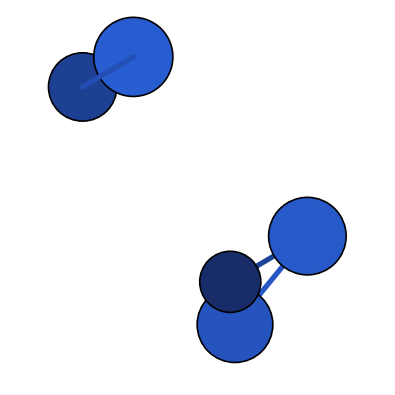
\includegraphics[width=0.85\linewidth]{figs/N5_anion_anion_005.png}\\[2pt]
{\small \texttt{N5\_anion\_anion\_005} -- C1}
\end{minipage}\hfill
\begin{minipage}{0.46\textwidth}
\centering
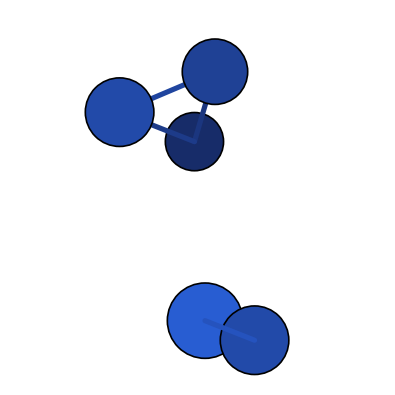
\includegraphics[width=0.85\linewidth]{figs/N5_anion_anion_007.png}\\[2pt]
{\small \texttt{N5\_anion\_anion\_007} -- C1}
\end{minipage}\hfill
\end{figure}
\begin{figure}[H]
\centering
\begin{minipage}{0.46\textwidth}
\centering
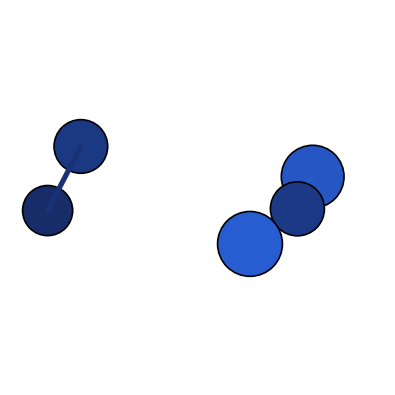
\includegraphics[width=0.85\linewidth]{figs/N5_anion_anion_008.png}\\[2pt]
{\small \texttt{N5\_anion\_anion\_008} -- C1}
\end{minipage}\hfill
\begin{minipage}{0.46\textwidth}
\centering
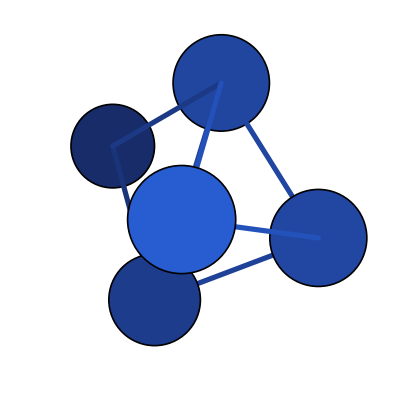
\includegraphics[width=0.85\linewidth]{figs/N5_anion_anion_010.png}\\[2pt]
{\small \texttt{N5\_anion\_anion\_010} -- C2v}
\end{minipage}\hfill
\end{figure}
\begin{figure}[H]
\centering
\begin{minipage}{0.46\textwidth}
\centering
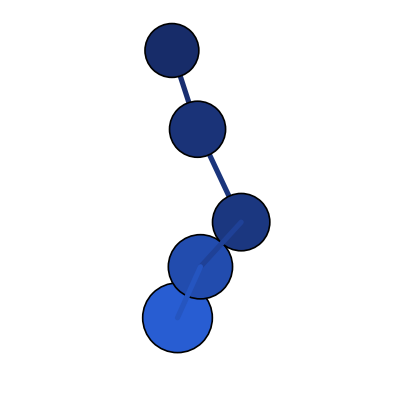
\includegraphics[width=0.85\linewidth]{figs/N5_cation_cation_001.png}\\[2pt]
{\small \texttt{N5\_cation\_cation\_001} -- C2v}
\end{minipage}\hfill
\begin{minipage}{0.46\textwidth}
\centering
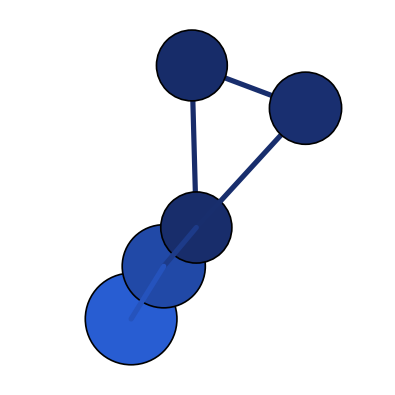
\includegraphics[width=0.85\linewidth]{figs/N5_cation_cation_002.png}\\[2pt]
{\small \texttt{N5\_cation\_cation\_002} -- Cs}
\end{minipage}\hfill
\end{figure}
\begin{figure}[H]
\centering
\begin{minipage}{0.46\textwidth}
\centering
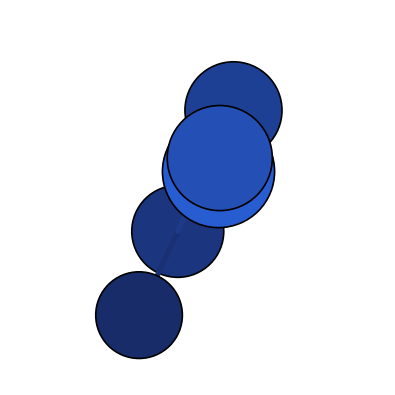
\includegraphics[width=0.85\linewidth]{figs/N5_cation_cation_004.png}\\[2pt]
{\small \texttt{N5\_cation\_cation\_004} -- C1}
\end{minipage}\hfill
\begin{minipage}{0.46\textwidth}
\centering
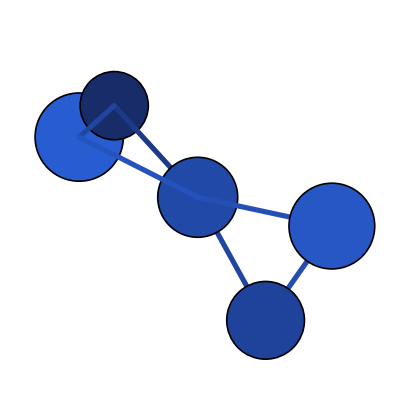
\includegraphics[width=0.85\linewidth]{figs/N5_cation_cation_005.png}\\[2pt]
{\small \texttt{N5\_cation\_cation\_005} -- D2d}
\end{minipage}\hfill
\end{figure}
\begin{figure}[H]
\centering
\begin{minipage}{0.46\textwidth}
\centering
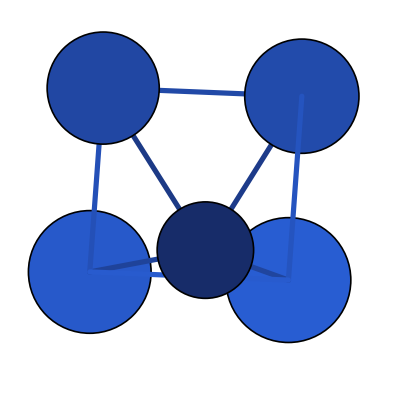
\includegraphics[width=0.85\linewidth]{figs/N5_cation_cation_006.png}\\[2pt]
{\small \texttt{N5\_cation\_cation\_006} -- C4v}
\end{minipage}\hfill
\begin{minipage}{0.46\textwidth}
\centering
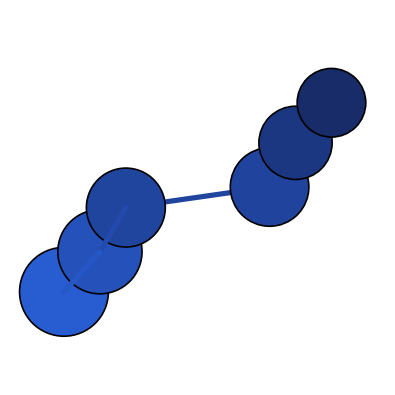
\includegraphics[width=0.85\linewidth]{figs/N6_neutral_neutral_001.png}\\[2pt]
{\small \texttt{N6\_neutral\_neutral\_001} -- C2}
\end{minipage}\hfill
\end{figure}
\begin{figure}[H]
\centering
\begin{minipage}{0.46\textwidth}
\centering
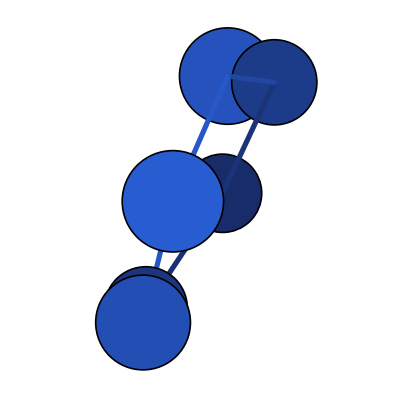
\includegraphics[width=0.85\linewidth]{figs/N6_neutral_neutral_002.png}\\[2pt]
{\small \texttt{N6\_neutral\_neutral\_002} -- D2}
\end{minipage}\hfill
\begin{minipage}{0.46\textwidth}
\centering
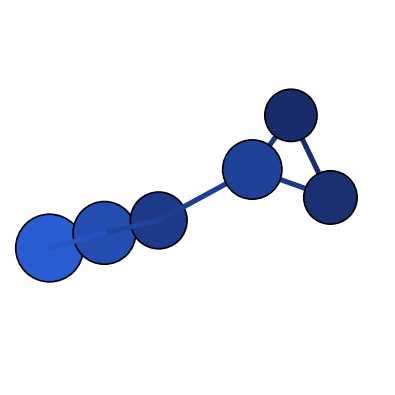
\includegraphics[width=0.85\linewidth]{figs/N6_neutral_neutral_003.png}\\[2pt]
{\small \texttt{N6\_neutral\_neutral\_003} -- C1}
\end{minipage}\hfill
\end{figure}
\begin{figure}[H]
\centering
\begin{minipage}{0.46\textwidth}
\centering
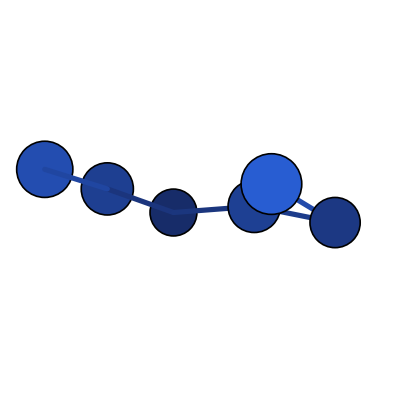
\includegraphics[width=0.85\linewidth]{figs/N6_neutral_neutral_006.png}\\[2pt]
{\small \texttt{N6\_neutral\_neutral\_006} -- C1}
\end{minipage}\hfill
\begin{minipage}{0.46\textwidth}
\centering
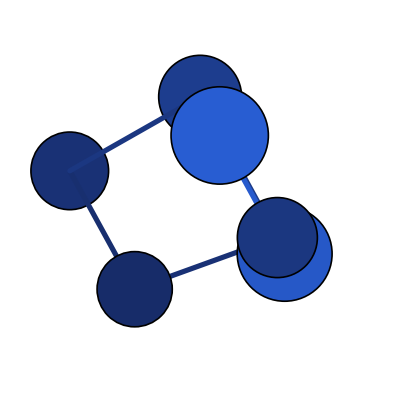
\includegraphics[width=0.85\linewidth]{figs/N6_neutral_neutral_007.png}\\[2pt]
{\small \texttt{N6\_neutral\_neutral\_007} -- C2}
\end{minipage}\hfill
\end{figure}
\begin{figure}[H]
\centering
\begin{minipage}{0.46\textwidth}
\centering
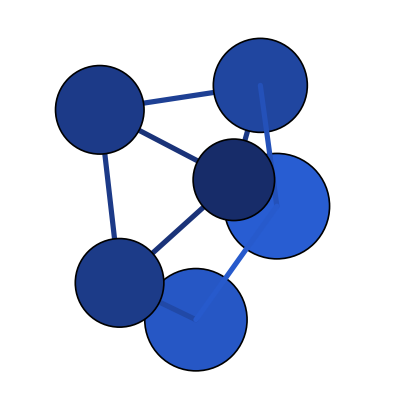
\includegraphics[width=0.85\linewidth]{figs/N6_neutral_neutral_008.png}\\[2pt]
{\small \texttt{N6\_neutral\_neutral\_008} -- C2v}
\end{minipage}\hfill
\begin{minipage}{0.46\textwidth}
\centering
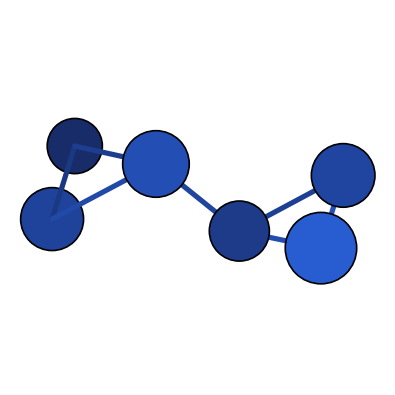
\includegraphics[width=0.85\linewidth]{figs/N6_neutral_neutral_009.png}\\[2pt]
{\small \texttt{N6\_neutral\_neutral\_009} -- C2}
\end{minipage}\hfill
\end{figure}
\begin{figure}[H]
\centering
\begin{minipage}{0.46\textwidth}
\centering
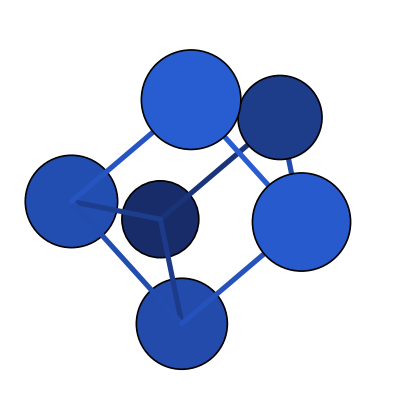
\includegraphics[width=0.85\linewidth]{figs/N6_neutral_neutral_012.png}\\[2pt]
{\small \texttt{N6\_neutral\_neutral\_012} -- D3h}
\end{minipage}\hfill
\begin{minipage}{0.46\textwidth}
\centering
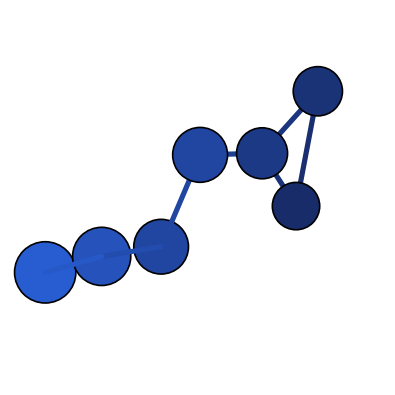
\includegraphics[width=0.85\linewidth]{figs/N7_anion_anion_008.png}\\[2pt]
{\small \texttt{N7\_anion\_anion\_008} -- C1}
\end{minipage}\hfill
\end{figure}
\begin{figure}[H]
\centering
\begin{minipage}{0.46\textwidth}
\centering
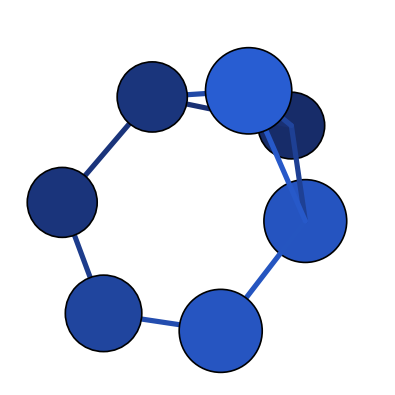
\includegraphics[width=0.85\linewidth]{figs/N7_anion_anion_010.png}\\[2pt]
{\small \texttt{N7\_anion\_anion\_010} -- C2v}
\end{minipage}\hfill
\begin{minipage}{0.46\textwidth}
\centering
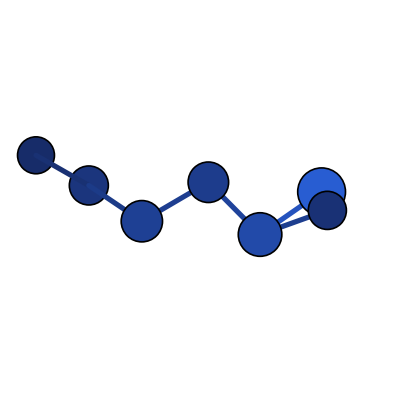
\includegraphics[width=0.85\linewidth]{figs/N7_anion_anion_011.png}\\[2pt]
{\small \texttt{N7\_anion\_anion\_011} -- C1}
\end{minipage}\hfill
\end{figure}
\begin{figure}[H]
\centering
\begin{minipage}{0.46\textwidth}
\centering
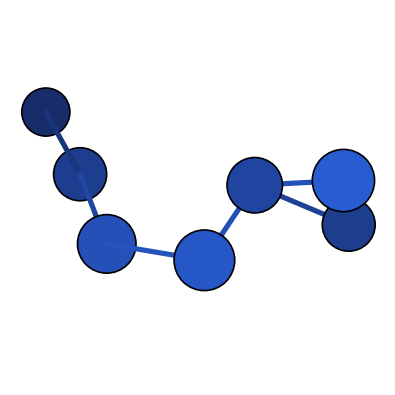
\includegraphics[width=0.85\linewidth]{figs/N7_anion_anion_012.png}\\[2pt]
{\small \texttt{N7\_anion\_anion\_012} -- C1}
\end{minipage}\hfill
\begin{minipage}{0.46\textwidth}
\centering
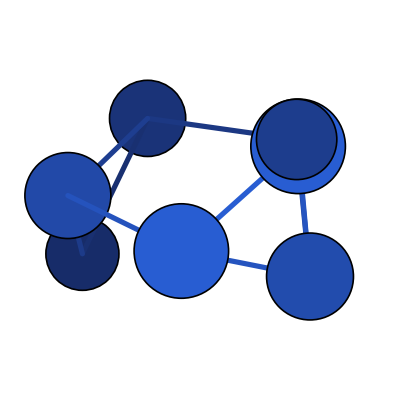
\includegraphics[width=0.85\linewidth]{figs/N7_anion_anion_019.png}\\[2pt]
{\small \texttt{N7\_anion\_anion\_019} -- C1}
\end{minipage}\hfill
\end{figure}
\begin{figure}[H]
\centering
\begin{minipage}{0.46\textwidth}
\centering
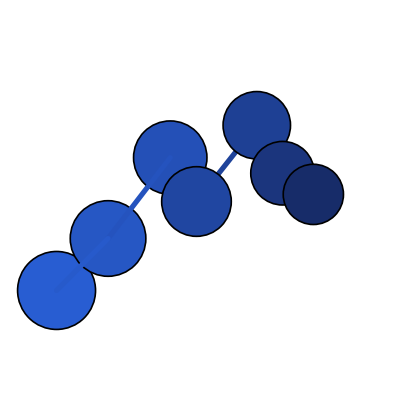
\includegraphics[width=0.85\linewidth]{figs/N7_cation_cation_001.png}\\[2pt]
{\small \texttt{N7\_cation\_cation\_001} -- Cs}
\end{minipage}\hfill
\begin{minipage}{0.46\textwidth}
\centering
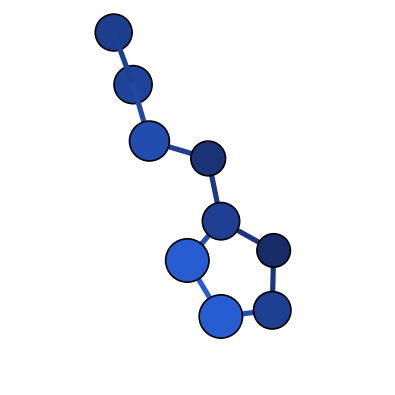
\includegraphics[width=0.85\linewidth]{figs/N9_anion_anion_001.png}\\[2pt]
{\small \texttt{N9\_anion\_anion\_001} -- C1}
\end{minipage}\hfill
\end{figure}
\begin{figure}[H]
\centering
\begin{minipage}{0.46\textwidth}
\centering
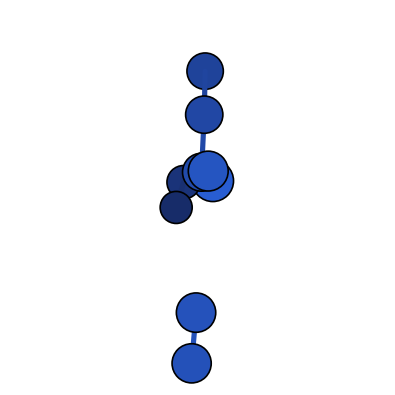
\includegraphics[width=0.85\linewidth]{figs/N9_cation_cation_001.png}\\[2pt]
{\small \texttt{N9\_cation\_cation\_001} -- C1}
\end{minipage}\hfill
\end{figure}

\clearpage
\subsection{R\'ef\'erences}
\label{sec:si-references}

Articles cit\'es dans les tableaux de la section~\ref{sec:provenance}
(num\'erotation propre \`a ce rapport ; correspondance avec les codes de
\texttt{biblio\_polyN/table\_references.tex} de \texttt{polyN-pipeline}
en annotation).

\begin{description}[leftmargin=1.6cm,itemsep=3pt,style=nextline]
\item[[1]] Fau, Mobita, Wilson, Perera, Bartlett, \emph{Quantum Theory Project report}, University of Florida.
\end{description}

\end{document}
